\documentclass[12pt,a4paper]{report}

% ── Pacchetti di base ────────────────────────────────────────────────────
\usepackage[utf8]{inputenc}
\usepackage[T1]{fontenc}
\usepackage[italian]{babel}
\usepackage[a4paper,margin=3cm]{geometry}
\usepackage{lmodern}
\usepackage{amsmath,amssymb}
\usepackage{mathrsfs}
\usepackage{graphicx}
\usepackage{subcaption}
\usepackage{booktabs}
\usepackage{rotating}
\usepackage{multirow}
\usepackage[expansion=false,nopatch=footnote]{microtype}
\usepackage{xcolor}
\usepackage{hyperref}
\usepackage{cleveref}
\usepackage[authoryear,round]{natbib}
\setlength{\marginparwidth}{2cm}
\usepackage[colorinlistoftodos]{todonotes}

% ── Link interni colorati ma senza le cornici colorate di default di
% hyperref (poco eleganti in stampa/PDF): colore unico, sobrio, per
% riferimenti, citazioni e URL ────────────────────────────────────────
\definecolor{linknavy}{RGB}{20,50,110}
\hypersetup{
  colorlinks=true,
  linkcolor=linknavy,
  citecolor=linknavy,
  urlcolor=linknavy,
  linktoc=all
}
\usepackage{setspace}
\onehalfspacing % interlinea 1.5
\usepackage{listings}
\usepackage{algorithm}
\usepackage{algpseudocode}
\setcounter{secnumdepth}{3}

% ── Stile per i listati di codice (sobrio: monocromatico, leggibile anche
% in stampa b/n, coerente con una tesi ingegneristica) ──────────────────
\definecolor{listinggray}{gray}{0.95}
\definecolor{listingcomment}{gray}{0.45}
\lstdefinestyle{thesiscode}{
  backgroundcolor=\color{listinggray},
  basicstyle=\ttfamily\small,
  commentstyle=\color{listingcomment}\itshape,
  keywordstyle=\bfseries,
  numbers=none,
  frame=single,
  rulecolor=\color{gray!60},
  framerule=0.4pt,
  breaklines=true,
  showstringspaces=false,
  columns=flexible,
  xleftmargin=1em,
  xrightmargin=1em,
  aboveskip=1em,
  belowskip=1em,
  language=bash
}
\lstset{style=thesiscode}

\graphicspath{{img/}{../results/plots/compare_3stat/}{../results/plots/differenza_percentuale/}{../results/plots/}}

% NOTA: stile bibliografico (natbib+plainnat) e classe (report) sono una
% scelta di default, non un requisito d'ateneo verificato — vedi piano_tesi.md
% §6. Da adattare se il template della sede impone altro (es. biblatex/biber,
% classe "book" con frontespizio dedicato).

% ── Dati del frontespizio ──────────────────────────────────────────────
% NOTA PER CHI COMPILA: i campi tra [ ] sono segnaposto, non dati reali —
% questo file non conosce il nome dell'ateneo, del corso di laurea, del
% relatore o del candidato. Sostituire prima della consegna.
\newcommand{\nomeUniversita}{Università di Firenze}
\newcommand{\nomeDipartimento}{Scuola di Scienze Matematiche Fisiche e Naturali}
\newcommand{\nomeCorso}{Laurea Magistrale in Data Science, Calcolo Scientifico \& Intelligenza Artificiale}
\newcommand{\nomeRelatore}{Daniele Castellana}
\newcommand{\nomeCandidato}{Alessio Minati}
\newcommand{\annoAccademico}{2025/2026}

\title{Apprendimento per Rinforzo Multi-Agente basato su Reti Neurali a Grafo per il Controllo Semaforico}
\author{}
\date{}

\begin{document}

% ── Frontespizio ─────────────────────────────────────────────────────────
\begin{titlepage}
  \centering
  \vspace*{0.5cm}
  {\large \nomeUniversita \par}
  \vspace{0.15cm}
  {\large \nomeDipartimento \par}
  \vspace{0.15cm}
  {\large \nomeCorso \par}

  \vspace{2.2cm}
  \rule{\textwidth}{0.6pt}\par
  \vspace{0.5cm}
  {\Huge \bfseries Apprendimento per Rinforzo Multi-Agente basato su Reti Neurali a Grafo per il Controllo Semaforico \par}
  %\vspace{0.4cm}
  %{\Large per il Controllo Semaforico Adattivo \par}
  \vspace{0.5cm}
  \rule{\textwidth}{0.6pt}\par

  \vspace{2.5cm}
  \begin{minipage}[t]{0.47\textwidth}
    \raggedright
    \large\textbf{Relatore}\par
    \normalsize\nomeRelatore\par
  \end{minipage}
  \hfill
  \begin{minipage}[t]{0.47\textwidth}
    \raggedleft
    \large\textbf{Candidato}\par
    \normalsize\nomeCandidato\par
  \end{minipage}

  \vfill
  {\large Anno Accademico \annoAccademico \par}
  \vspace{0.5cm}
\end{titlepage}

% ── Pagina bianca (recto/verso del frontespizio) ─────────────────────────
\newpage
\thispagestyle{empty}
\null
\newpage

% ── Front matter: numerazione romana ─────────────────────────────────────
\pagenumbering{roman}

%!TEX root = ../mainufficiale.tex
\chapter*{Sommario}
\addcontentsline{toc}{chapter}{Sommario}

Il traffico veicolare nelle aree urbane attraversa incroci regolati da
semafori, e il modo in cui le fasi vengono decise incide sui tempi di
percorrenza e sulla congestione della rete. Le soluzioni classiche, dai
piani a tempi fissi ai sistemi coordinati come SCOOT e SCATS, si basano
su euristiche definite manualmente e restano per questo poco flessibili
di fronte a condizioni di traffico diverse da quelle previste in fase di
progettazione. Il reinforcement learning offre un'alternativa,
apprendendo una politica di controllo dall'esperienza simulata; le
architetture più recenti coordinano gli agenti di intersezioni vicine
tramite reti neurali a grafo, ma tendono a concentrarsi sull'efficienza
aggregata, senza trattare l'equità tra le direzioni di traffico come
obiettivo esplicito né verificare sistematicamente la generalizzazione a
condizioni mai osservate in addestramento.

Questo lavoro usa come punto di partenza MetaSTGAT, un'architettura in
cui ogni incrocio è controllato da un agente che apprende e gli agenti si
scambiano informazioni con gli incroci vicini tramite una rete neurale a
grafo, per condurre uno studio sperimentale del compromesso tra
efficienza, equità e generalizzazione. L'ambiente, costruito su CityFlow,
riproduce reti a griglia di tre dimensioni con traffico generato
parametricamente; il confronto include le baseline Fixed-Time e
Max-Pressure ed è organizzato in tre studi indipendenti, sul peso
assegnato all'equità nella ricompensa, su un'ablazione sistematica delle
modifiche introdotte, e sul meccanismo di comunicazione tra intersezioni.
Ogni modello è valutato, senza riaddestramento, su topologie, spaziature
e profili di traffico mai incontrati in addestramento.

Il modello di riferimento riduce l'attesa massima subita dai veicoli del
59\% in addestramento e del 52\% in valutazione rispetto a Max-Pressure,
a fronte di un tempo di percorrenza medio superiore di pochi punti
percentuali. Sulle topologie più grandi mai viste in addestramento,
Max-Pressure arriva a bloccare almeno un veicolo per l'intera durata
dell'episodio in ogni configurazione testata, mentre il modello di
riferimento resta entro limiti nettamente più contenuti. L'ablazione
mostra inoltre che questo vantaggio dipende dalla combinazione tra il
segnale di attesa nello stato e il termine dedicato nella ricompensa, non
da un singolo dettaglio dell'algoritmo di apprendimento.

Questi risultati indicano che l'equità tra direzioni di traffico può
essere perseguita senza una rinuncia sostanziale all'efficienza, e che
parte di questo vantaggio si conserva su condizioni diverse da quelle di
addestramento.


\tableofcontents
\listoffigures
\listoftables

%!TEX root = ../mainufficiale.tex
\chapter*{Acronimi e Notazione}
\addcontentsline{toc}{chapter}{Acronimi e Notazione}

\section*{Acronimi}
\begin{table}[ht]
\centering
\small
\begin{tabular}{@{}ll@{}}
\toprule
Acronimo & Significato \\
\midrule
MDP & Markov Decision Process \\
RL & Reinforcement Learning \\
DQN & Deep Q-Network \\
PER & Prioritized Experience Replay \\
BPTT & Backpropagation Through Time \\
GNN & Graph Neural Network \\
GCN & Graph Convolutional Network \\
GAT & Graph Attention Network \\
TSC & Traffic Signal Control \\
SMK & Spatial Meta-Knowledge (learner) \\
TMK & Temporal Meta-Knowledge (learner) \\
CS & Cooperation Spatial (modulo Meta-GAT) \\
CST & Cooperation Spatial-Temporal (modulo Meta-GAT) \\
\bottomrule
\end{tabular}
\end{table}

\newpage
\section*{Notazione principale}
\begin{table}[ht]
\centering
\small
\begin{tabular}{@{}lp{10.5cm}@{}}
\toprule
Simbolo & Significato \\
\midrule
$\mathcal{S}, \mathcal{A}, P, R, \gamma$ & Stati, azioni, transizione, ricompensa, sconto \\
$\pi$, $V^\pi$, $Q^\pi$ & Politica, funzione valore-stato, funzione valore-azione \\
$\theta$, $\theta^-$ & Pesi della rete online e della target network \\
$\tau$ & Coefficiente di soft update \\
$\alpha$ (in RL) & Esponente di prioritizzazione del PER \\
$\alpha$ (in questo lavoro) & Peso della penalità anti-starvation nella ricompensa \\
$\varepsilon$ & Probabilità di esplorazione \\
$s_i^t, a_i^t, r_i^t$ & Stato, azione, ricompensa dell'intersezione $i$ al tempo $t$ \\
$n_i^t, w_i^t, p_i^t$ & Veicoli per corsia, attesa massima per corsia, fase corrente \\
$d_0$ & Dimensione dello stato in ingresso \\
$d_1$ & Dimensione nascosta del modello \\
$H$, $d_h$ & Numero di teste di attenzione e dimensione per testa \\
$e_i^t, e_j^t$ & Embedding temporale e spaziale del Dual State Encoder \\
$x_i^t, h_i^t, c_i^t$ & Output, stato nascosto e stato di cella del Meta-LSTM \\
$\mathrm{SMK}(i), \mathrm{TMK}(i)$ & Meta-embedding spaziale e temporale dell'intersezione $i$ \\
$z_{\mathrm{CS}}(i), z_{\mathrm{CST}}(i)$ & Output dei moduli Meta-GAT spaziale e spazio-temporale \\
$\overline{tt}$, $tt_{\max}$ & Travel time medio e massimo \\
$tc$ & Trip completion, percentuale di veicoli che completano il percorso \\
$\text{wait}_{\max}$ & Max wait, tempo massimo di un veicolo sulla stessa corsia senza superare l'incrocio \\
\bottomrule
\end{tabular}
\end{table}


% ── Corpo della tesi: numerazione araba da qui ────────────────────────────
\cleardoublepage
\pagenumbering{arabic}

%!TEX root = ../mainufficiale.tex
\chapter{Introduzione}
\label{cap:introduzione}

\section{Contesto e motivazioni}
\label{sec:intro-motivazioni}

Il traffico veicolare nelle aree urbane attraversa la rete stradale
passando per una sequenza di incroci regolati da semafori. Il modo in cui
le fasi vengono decise incide direttamente sui tempi di percorrenza e
sulla congestione complessiva della rete, rendendo il controllo
semaforico un problema di interesse pratico oltre che di ricerca.

Un incrocio semaforizzato stabilisce periodicamente quali flussi
veicolari autorizzare e quali arrestare.
Su una singola intersezione il problema è garantire che i veicoli in attesa continuino a scorrere in modo regolare.
Le soluzioni classiche affrontano questo compito in due modi: un piano a
tempi fissi che ripete una sequenza di fasi di durata prestabilita, calcolata
una tantum su stime di traffico medie e mai più rivista in tempo reale, e un
controllo attuato dai sensori che concede il verde a una direzione solo
quando un sensore rileva la presenza di un veicolo in coda, adattandosi
così, entro certi limiti, alle variazioni del traffico osservato.

Se si considera una rete composta da più incroci, il problema cambia
natura. La fase scelta a un'intersezione influenza, con un ritardo
proporzionale alla distanza, il volume di veicoli in arrivo alle
intersezioni adiacenti, per cui le decisioni prese nei singoli punti della
rete non possono più essere indipendenti tra loro. Sistemi come SCOOT e
SCATS rispondono a questa esigenza da diversi decenni, aggiustando
periodicamente i piani semaforici di un'intera area urbana sulla base del
traffico rilevato in tempo reale \citep{wei2020tscsurvey}. Il controllo
semaforico su rete si configura quindi come un problema di coordinamento
distribuito, inteso come la necessità per un insieme di processi autonomi
di concordare su un'azione comune e coerente senza un'autorità centrale.

Entrambe le famiglie di soluzioni, dai piani a tempi fissi ai sistemi
coordinati come SCOOT e SCATS, si basano su euristiche definite
manualmente e restano per questo poco flessibili di fronte a condizioni
di traffico diverse da quelle previste in fase di progettazione.

Valutare un controllore semaforico richiede di tenere conto di due
proprietà distinte. La prima è l'efficienza, la capacità di ridurre il
tempo che i veicoli impiegano ad attraversare la rete. La seconda è
l'equità, la garanzia che nessuna direzione di traffico venga fatta
attendere sistematicamente più a lungo delle altre. Le due proprietà non sono la
stessa cosa e non migliorano necessariamente insieme. Un controllore può
massimizzare il flusso complessivo e allo stesso tempo lasciare una
minoranza di veicoli bloccata a lungo, se la sua logica di decisione non
include alcuna attenzione esplicita al caso peggiore. In questo studio
dunque un controllore che fa aspettare pochi veicoli molto a lungo non è
preferibile a uno leggermente più lento in media ma che non lascia mai
nessuno bloccato per un tempo indefinito.

Le soluzioni proposte per affrontare questo compromesso si dividono in due
famiglie. Da un lato regole scritte a mano come \textsc{Max-Pressure}
\citep{varaiya2013maxpressure}, che selezionano a ogni istante la fase
capace di liberare più veicoli di quanti ne farebbe accumulare: un
approccio dimostrabilmente efficiente nel lungo periodo, ma per
costruzione miope rispetto all'equità, poiché ottimizza sempre il valore
istantaneo più alto senza mai considerare da quanto tempo attende la
direzione esclusa. Dall'altro il controllo appreso tramite reinforcement
learning, dove una politica viene addestrata a massimizzare una
ricompensa invece di seguire una regola scritta a mano. Applicato a una
rete di più intersezioni, un'architettura recente affida a ogni incrocio
un agente che apprende, mentre gli agenti si scambiano informazioni con
gli incroci vicini attraverso una rete neurale a grafo, permettendo a
ciascuna intersezione di condizionare la propria decisione sullo stato
dei vicini senza una politica centralizzata. Le architetture di questo
tipo, tra cui MetaSTGAT \citep{wang2022metastgat}, il modello di
riferimento di questo lavoro, raggiungono buoni risultati di efficienza
aggregata, ma tipicamente non trattano l'equità come obiettivo esplicito
di progettazione né verificano sistematicamente la generalizzazione a
topologie mai osservate in addestramento. Questo lavoro si concentra
proprio su questa famiglia di approcci, reinforcement learning coordinato
tramite reti neurali a grafo, usando MetaSTGAT come architettura di
partenza.

\section{Obiettivi e domande di ricerca}

L'obiettivo di questo lavoro è indagare sperimentalmente se, e a quali
condizioni, un controllore appreso di questo tipo possa perseguire
efficienza ed equità congiuntamente, mantenendo le prestazioni osservate
anche su condizioni mai incontrate in addestramento.

A questo scopo, questo lavoro usa l'architettura di MetaSTGAT come punto
di partenza, introducendo un termine dedicato della ricompensa che
penalizza l'attesa massima osservata su una corsia non ancora servita
dalla fase corrente, applicato a ogni singolo passo di decisione e per
ogni intersezione. Per verificare se questo meccanismo funzioni davvero,
la valutazione si affida a una metrica puramente osservazionale,
calcolata allo stesso modo per ogni controllore indipendentemente da come
è stato addestrato: il tempo massimo che un veicolo qualunque trascorre
sulla stessa corsia senza superare l'incrocio, in una qualunque
intersezione della rete.

Questo lavoro esplora tre domande di ricerca.
\begin{enumerate}
    \item Un controllore appreso e coordinato tramite reti neurali a grafo
          può ridurre l'attesa massima subita dai veicoli rispetto a un
          controllore puramente reattivo come \textsc{Max-Pressure}? E a
          quale costo in termini di efficienza media?
    \item Tale vantaggio si mantiene su topologie di rete, spaziature
          stradali e profili di traffico mai incontrati in addestramento?
    \item Quali tra le scelte progettuali e le modifiche studiate in
          questo lavoro, dal meccanismo di comunicazione spaziale ai
          dettagli della procedura di addestramento, contribuiscono
          effettivamente al comportamento osservato?
\end{enumerate}

\section{Contributi di questo lavoro}

Nello specifico, i contributi di questa tesi sono i seguenti.

\paragraph{Un ambiente di simulazione multi-intersezione riproducibile.}
Questa tesi costruisce da zero un ambiente su \textsc{CityFlow}
\citep{zhang2019cityflow}, con reti stradali a griglia di dimensione
$4\times4$, $5\times5$ e $6\times6$, due spaziature stradali distinte,
otto fasi semaforiche per intersezione, insieme a una
generazione parametrica dei dati di traffico con profili a intensità
costante, a gradino e a giornata lavorativa. In ogni configurazione il
traffico su una riga della griglia è potenziato artificialmente per
simulare un'arteria stradale, condizione necessaria per poter osservare
uno squilibrio direzionale in caso di traffico asimmetrico.

\paragraph{Uno studio sistematico del compromesso tra efficienza ed
    equità.} Variando il peso assegnato alla componente di equità nella
ricompensa, questa tesi quantifica direttamente il compromesso che il
meccanismo introduce, mostrando in particolare che rimuoverlo del tutto
non produce il guadagno di efficienza che ci si potrebbe attendere, pur
restando il controllore appreso nettamente al di sotto di
\textsc{Max-Pressure} e Fixed-Time sulle metriche di caso peggiore.

\paragraph{Uno studio di ablazione sull'origine del comportamento
    osservato.} Questa tesi isola singolarmente ciascuna delle modifiche
introdotte rispetto alla procedura di riferimento, dal meccanismo di
stato e ricompensa fino ai dettagli dell'algoritmo di apprendimento,
invece di presentarle come un insieme indistinto di miglioramenti, per
valutare empiricamente il contributo di ciascuna al comportamento
osservato.

\paragraph{Un confronto tra meccanismi di comunicazione spaziale a parità
    di resto dell'architettura.} Questa tesi confronta tre meccanismi di
comunicazione tra intersezioni, \emph{graph attention}, \emph{graph convolution} e propagazione a onda ispirata a SONAR \citep{trenta2025sonar}, mantenendo identico il
resto dell'architettura, per verificare se il comportamento osservato
dipenda specificamente dal meccanismo di attenzione appreso o sia una
proprietà più generale della coordinazione locale via rete neurale a
grafo.

\paragraph{Un protocollo di valutazione a generalizzazione sistematica.}
Ogni modello di questa tesi, appreso o classico, è valutato senza
riaddestramento su topologie, spaziature e profili di traffico mai
incontrati in addestramento, riportando media e caso peggiore del tempo
di viaggio, la percentuale di veicoli che completano il proprio percorso
e la massima attesa registrata da un veicolo allo stesso incrocio.

\section{Struttura della tesi}

Il Capitolo~\ref{cap:background} introduce il background necessario a
leggere i capitoli successivi senza assumere familiarità pregressa con
nessuno dei campi coinvolti, dal reinforcement learning alle reti neurali
ricorrenti, dalle reti neurali a grafo al controllo semaforico. Il
Capitolo~\ref{cap:tsc-modelli} formalizza il problema affrontato,
presenta l'architettura di MetaSTGAT e le modifiche studiate in questo
lavoro, i meccanismi di comunicazione spaziale alternativi e la procedura
di addestramento adottata, e descrive infine l'ambiente di simulazione.
Il Capitolo~\ref{cap:confronto} descrive il protocollo sperimentale e
riporta i risultati ottenuti sui tre studi, peso dell'equità, ablation,
meccanismi spaziali. Il Capitolo~\ref{cap:conclusioni} discute i
risultati alla luce degli obiettivi dichiarati in questa introduzione,
indica le direzioni lasciate aperte e dichiara i limiti dello studio.

%!TEX root = ../mainufficiale.tex
\chapter{Background}
\label{cap:background}

Questo capitolo introduce i concetti necessari per leggere i
Capitoli~\ref{cap:tsc-modelli} e \ref{cap:confronto} senza assumere
familiarità pregressa con i campi coinvolti. Si parte dalle reti neurali
e dal loro addestramento (§\ref{sec:background-nn}), per poi presentare
il reinforcement learning, dal paradigma agente-ambiente alle estensioni
del DQN usate in questo lavoro (§\ref{sec:background-rl}), le reti
neurali ricorrenti (§\ref{sec:background-rnn}) e le reti neurali a grafo,
incluse le formulazioni confrontate sperimentalmente nel
Capitolo~\ref{cap:confronto} (§\ref{sec:background-gnn}). Il capitolo si
chiude presentando il controllo semaforico come problema applicativo, la
letteratura che lo affronta e ciò che resta aperto
(§\ref{sec:background-tsc}).

\section{Reti Neurali}
\label{sec:background-nn}

Una \textbf{rete neurale} è una funzione parametrica che trasforma un input in un output attraverso una successione di funzioni matematiche, i cui parametri, chiamati pesi, vengono appresi dai dati invece di essere codificati manualmente.
L'unità base è il \emph{neurone artificiale} o \emph{percettrone}, mostrato in Figura~\ref{fig:percettrone}:
esso riceve un vettore di input $x = (x_1, x_2, \dots, x_n) \in \mathbb{R}^n$,
ne calcola una combinazione lineare pesata $z = w^\top x + b = \sum_{i=1}^{n} w_i x_i + b$
(con $w = (w_1, w_2, \dots, w_n) \in \mathbb{R}^n$ il vettore di pesi e $b \in \mathbb{R}$ un termine costante detto \emph{bias}),
e applica a $z$ una funzione non lineare $\sigma$ detta \emph{funzione di attivazione},
producendo l'output $\hat{y}=\sigma(z)$.

\begin{figure}[htbp]
  \centering
  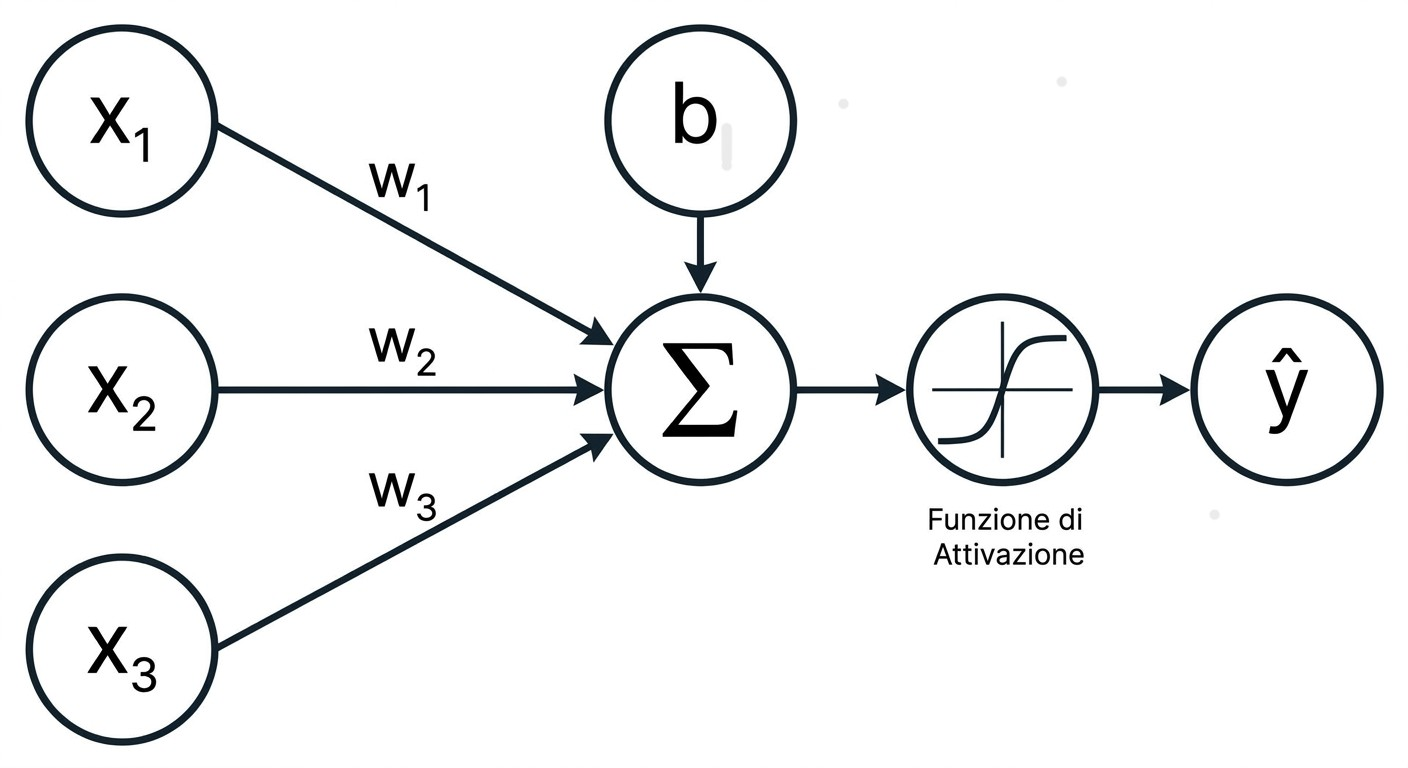
\includegraphics[width=0.7\textwidth]{nn_percettrone.jpg}
  \caption{Il percettrone: gli input $x_1, x_2, x_3$ vengono combinati con i
    pesi $w_1, w_2, w_3$ e il bias $b$, la somma $z$ attraversa la funzione
    di attivazione, producendo l'output $\hat y$.}
  \label{fig:percettrone}
\end{figure}

Attivazioni comuni, mostrate in Figura~\ref{fig:attivazioni}, sono la sigmoide $\sigma(z) = 1/(1+e^{-z})$, che comprime $z$ in $(0,1)$,
la tangente iperbolica $\tanh(z) = (e^z - e^{-z})/(e^z + e^{-z})$, che lo comprime invece in $(-1,1)$,
e la ReLU (Rectified Linear Unit) $\max(0,z)$, che si limita ad azzerare i valori negativi.
La non linearità è essenziale: senza di essa, comporre più trasformazioni lineari
produrrebbe comunque una singola trasformazione lineare, non riuscendo ad apprendere delle relazioni complesse e non lineari presenti nei dati.

\begin{figure}[htbp]
  \centering
  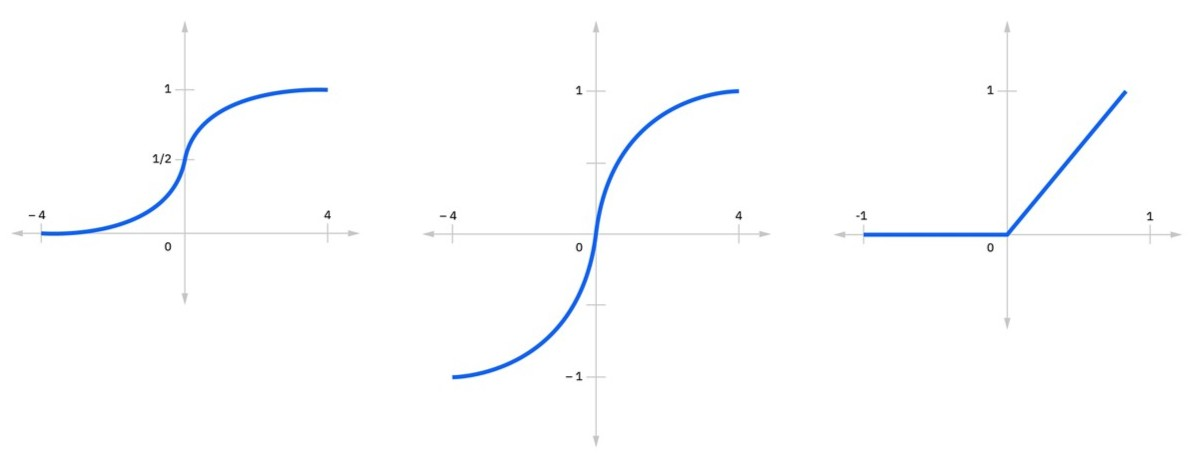
\includegraphics[width=0.85\textwidth]{nn_attivazioni.jpeg}
  \caption{Le tre funzioni di attivazione discusse: sigmoide, tangente
    iperbolica e ReLU.}
  \label{fig:attivazioni}
\end{figure}

Una rete neurale \emph{feedforward} o \emph{multi-layer perceptron} (MLP)
dispone i neuroni in \textbf{strati} (\emph{layer}) successivi: l'output
di ogni strato è l'input dello strato seguente, dall'\emph{input layer}
(i dati grezzi) attraverso uno o più \emph{hidden layer} fino
all'\emph{output layer} finale, come in Figura~\ref{fig:mlp}.
In forma matriciale, un singolo layer calcola
\[h^{(l+1)} = \sigma\!\left(W^{(l)} h^{(l)} + b^{(l)}\right)\]
dove
$h^{(l)}$ raccoglie gli output di tutti i neuroni dello strato $l$,
$W^{(l)}$ è la matrice che impila i pesi di ciascun neurone di quello strato e
$b^{(l)}$ è il vettore dei bias.
Impilare più strati permette alla rete di comporre trasformazioni via via più astratte dell'input originale.

\begin{figure}[htbp]
  \centering
  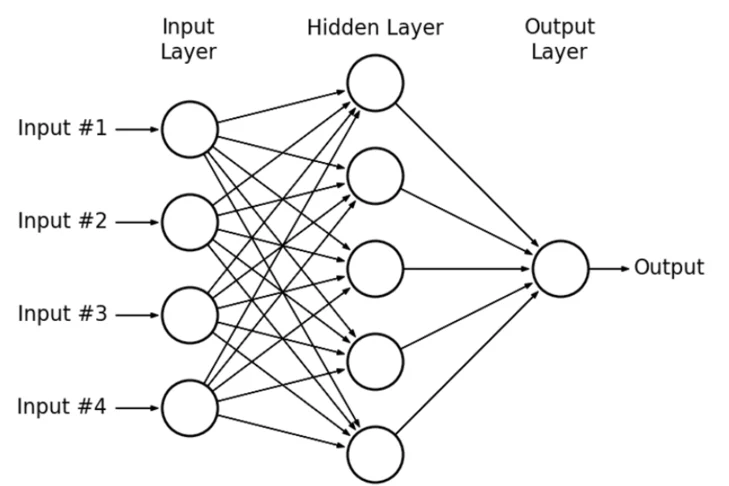
\includegraphics[width=0.6\textwidth]{nn_mlp.png}
  \caption[Una rete feedforward con un input layer a 4 nodi, un hidden layer a 5 nodi e un output layer a un nodo.]{Una rete feedforward con un input layer a 4 nodi, un hidden
    layer a 5 nodi e un output layer a un nodo: ogni connessione porta con
    sé un peso appreso, omesso per chiarezza. Fonte: Wikimedia
    Commons.\footnote{\url{https://commons.wikimedia.org/wiki/File:Neural_Network.gif}}}
  \label{fig:mlp}
\end{figure}

\paragraph{Addestramento: discesa del gradiente e backpropagation.}
Una rete neurale viene inizializzata con pesi e bias casuali e viene addestrata
iterativamente confrontando l'output prodotto con quello desiderato.
Una funzione di loss $\mathcal{L}(\hat y, y)$ quantifica la distanza tra l'output prodotto $\hat y$ e quello desiderato
$y$ (che sia esso una etichetta di classificazione o un valore reale nel caso della regressione).
L'addestramento consiste nel regolare ogni peso nella direzione che riduce $\mathcal{L}$, un'operazione
nota come \emph{discesa del gradiente}:
\[w \leftarrow w - \eta \frac{\partial \mathcal{L}}{\partial w},\]
dove $\eta$, il \emph{tasso di apprendimento} o \emph{learning rate}, controlla l'ampiezza di ogni aggiornamento.
Calcolare la derivata parziale $\partial \mathcal{L}/\partial w$ per ogni peso della rete, dal più vicino
all'output al più lontano, richiede applicare ripetutamente la \emph{chain rule} del calcolo differenziale attraverso tutti gli strati
intermedi: l'algoritmo che esegue questo calcolo in modo efficiente, una
sola passata dall'output verso l'input, è la \emph{backpropagation} \citep{rumelhart1986backprop}.
Nella pratica, il gradiente non è esatto ma si stima su un piccolo sottoinsieme casuale di
dati (\emph{mini-batch}) alla volta invece che sull'intero insieme di
dati disponibile, una variante nota come discesa del gradiente
stocastica, molto più economica computazionalmente a fronte di una stima
del gradiente più rumorosa ma sufficiente a guidare comunque
l'addestramento verso una soluzione utile.

\paragraph{Oltre la discesa del gradiente pura.} La regola di
aggiornamento vista sopra usa lo stesso tasso di apprendimento $\eta$ per
ogni peso della rete, un limite quando la superficie di loss ha curvatura
molto diversa da un peso all'altro (alcune direzioni richiederebbero un
passo grande, altre uno minimo): un ottimizzatore più sofisticato adatta
l'ampiezza dell'aggiornamento parametro per parametro, sulla base della
storia recente dei gradienti osservati.
Il \emph{momentum} \citep{qian1999momentum} accumula una
media mobile esponenziale dei gradienti passati e aggiorna i pesi in quella
direzione media invece che nella sola direzione del gradiente corrente,
smorzando le oscillazioni lungo le direzioni in cui il segno del gradiente
cambia di continuo. \textbf{RMSprop} \citep{tieleman2012rmsprop} adotta un
principio complementare: mantiene per ciascun peso una media mobile del
quadrato dei gradienti recenti e divide l'aggiornamento per la sua radice,
riducendo il passo sui pesi il cui gradiente è stato storicamente grande in
valore assoluto e aumentandolo su quelli il cui gradiente è stato piccolo,
così da rendere il progresso più uniforme tra pesi con scale molto diverse.
\textbf{Adam} \citep{kingma2015adam}, un altro ottimizzatore molto usato, combina invece entrambe le idee, media mobile
del gradiente e del suo quadrato. Questo lavoro
adotta \textbf{RMSprop}, coerentemente con il modello di riferimento
\citep{wang2022metastgat}, per l'addestramento delle proprie reti neurali.

Ogni rete usata in questo lavoro, dal DQN (§\ref{sec:background-rl}) alla
LSTM (§\ref{sec:background-rnn}) alle reti a grafo
(§\ref{sec:background-gnn}), è in ultima analisi una particolare
composizione di questi stessi due ingredienti: strati di neuroni con
un'attivazione non lineare, addestrati per discesa del gradiente tramite
backpropagation. Ciò che cambia da un'architettura all'altra è come gli
strati sono collegati tra loro, non il principio di addestramento
sottostante.

\section{Reinforcement Learning}
\label{sec:background-rl}

\subsection{Il paradigma agente-ambiente}

L'apprendimento per rinforzo o \emph{reinforcement learning} (RL) è un
paradigma di apprendimento automatico in cui un \emph{agente} impara un
certo comportamento interagendo ripetutamente con un \emph{ambiente}, senza che
gli siano forniti esempi di comportamento corretto. A ogni passo di
tempo $t$, l'agente osserva lo stato corrente dell'ambiente, sceglie
un'\emph{azione} tra quelle disponibili, e riceve in cambio due informazioni:
un nuovo stato (l'ambiente è cambiato, anche per effetto dell'azione
scelta) e un numero scalare, la \emph{ricompensa}, che indica quanto
quell'azione sia stata desiderabile in quel momento.
Il problema che il RL affronta è per l'appunto
questo, cioè imparare per tentativi ripetuti quale comportamento massimizzi
la somma delle ricompense ricevute nel tempo, non solo quella immediata.
La Figura~\ref{fig:rl-loop} riassume questo ciclo, utile come riferimento
per la terminologia introdotta nel resto della sezione.

\begin{figure}[htbp]
  \centering
  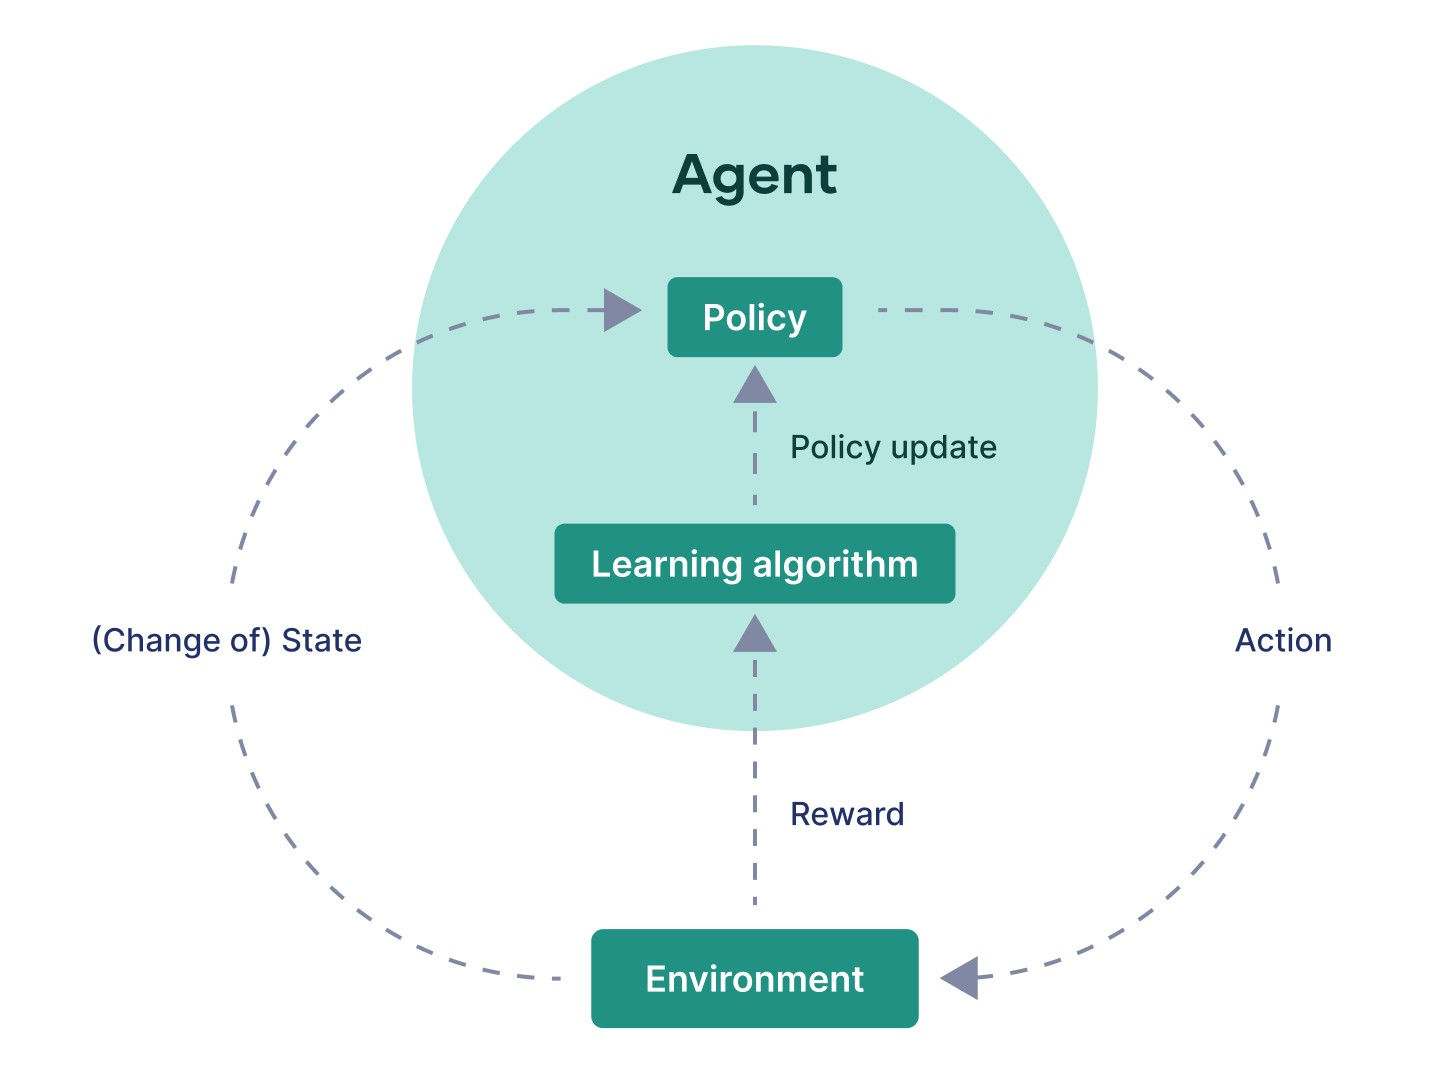
\includegraphics[width=0.55\textwidth]{rl_loop}
  \caption[Il ciclo agente-ambiente.]{Il ciclo agente-ambiente: la policy sceglie un'azione,
    l'ambiente risponde con un nuovo stato e una ricompensa, e
    l'algoritmo di apprendimento usa quella ricompensa per aggiornare la
    policy. Fonte: adattata da un articolo
    Medium.\footnote{\url{https://medium.com/the-curious-algorithm/a-straightforward-introduction-to-artificial-intelligence-b39f8d9152c2}}}
  \label{fig:rl-loop}
\end{figure}

Vale la pena distinguere questo paradigma da quello dell'\emph{apprendimento
  supervisionato}. In quest'ultimo una rete neurale riceve coppie input-output correttamente associate e impara
a riprodurre quella corrispondenza. Nel RL non esiste alcuna etichetta
corretta da imitare: l'agente deve scoprire da solo, per tentativi, quale
azione sia buona in ciascuno stato, guidato solo dalla
ricompensa ricevuta in seguito alla azione che l'ha causata.
È un problema strutturalmente più difficile,
ma anche particolarmente adatto a situazioni, come il controllo semaforico, in
cui nessuno conosce a priori quale sia la "decisione corretta" da
etichettare.

\subsection{Processo decisionale di Markov}

La formalizzazione matematica standard di un problema di RL è il
\emph{processo decisionale di Markov} (MDP) \citep{suttonbarto2018},
definito dalla tupla
\[\mathcal{M} = (\mathcal{S}, \mathcal{A}, P, R, \gamma)\]
dove $\mathcal{S}$ è l'insieme di tutti gli stati possibili dell'ambiente,
$\mathcal{A}$ l'insieme di tutte le azioni possibili, $P(s' \mid s,a)$ la
probabilità di transitare nello stato $s'$ avendo eseguito l'azione $a$
nello stato $s$, $R(s,a)$ la ricompensa attesa per quella stessa coppia, e
$\gamma \in [0,1)$ il \emph{fattore di sconto}, che pondera l'importanza
delle ricompense future rispetto a quelle immediate: un $\gamma$ vicino a
$0$ rende l'agente "miope", interessato quasi solo alla ricompensa
immediata, un $\gamma$ vicino a $1$ lo rende attento anche a conseguenze
lontane nel tempo. Questa formalizzazione si basa sull'assunzione di Markov, per la quale la
probabilità di transizione $P(s'\mid s,a)$ dipende solo dallo stato
corrente $s$ e non dalla sequenza di stati che ha portato allo stesso.

Un agente segue una \emph{politica} $\pi(a \mid s)$, una distribuzione
di probabilità sulle azioni condizionata allo stato corrente; il suo
obiettivo è massimizzare il \emph{ritorno} atteso
\[G_t = \sum_{k=0}^{\infty} \gamma^k r_{t+k}\]
ovvero la somma scontata delle ricompense future a partire dall'istante
$t$. Per poter ragionare su quanto buona sia una politica prima ancora di
eseguirla fino in fondo, si definiscono due funzioni valore: la
funzione valore-stato $V^\pi(s) = \mathbb{E}_\pi[G_t \mid s_t = s]$ e la
funzione valore-azione $Q^\pi(s,a) = \mathbb{E}_\pi[G_t \mid s_t=s,
    a_t=a]$, che misurano rispettivamente quanto ritorno atteso si ottiene
seguendo $\pi$ da uno stato, o da una coppia stato-azione. Queste
soddisfano l'\emph{equazione di Bellman}, che esprime il valore di uno
stato in funzione del valore atteso degli stati successivi:
\begin{equation}
  V^\pi(s) = \sum_a \pi(a\mid s) \sum_{s'} P(s'\mid s,a) \big[R(s,a) + \gamma V^\pi(s')\big]
\end{equation}
Per una politica ottima $\pi^*$ che massimizza $V^\pi(s)$ per ogni stato
simultaneamente, vale l'analoga equazione di Bellman di ottimalità:
\begin{equation}
  Q^*(s,a) = \mathbb{E}_{s' \sim P(\cdot \mid s,a)}\left[
    R(s,a) + \gamma \max_{a'} Q^*(s', a')
    \right]
  \label{eq:bellman-optimal}
\end{equation}
Se si conoscesse $Q^*$, la politica ottima sarebbe immediata da ricavare:
scegliere sempre $\operatorname*{argmax}_a Q^*(s,a)$. Il problema del RL
si riduce quindi, in buona parte, a stimare $Q^*$ senza conoscerlo a
priori.

\subsection{Apprendimento model-based e model-free}
\label{subsec:model-free}

Esiste una distinzione fondamentale tra due famiglie di algoritmi RL, a
seconda che l'agente costruisca o meno una rappresentazione esplicita
della dinamica dell'ambiente. Un algoritmo \emph{model-based} apprende
o riceve un modello approssimato di $P(s'\mid s,a)$ e $R(s,a)$, e lo usa
per simulare le conseguenze di più
sequenze di azioni prima di sceglierne una, senza eseguirle davvero nell'ambiente.
Un algoritmo \emph{model-free}, al contrario, non costruisce alcun modello della dinamica dell'ambiente, bensì stima
direttamente $Q^*$ dall'esperienza osservata, senza mai
provare a prevedere esplicitamente lo stato successivo. Il vantaggio del
model-free è la semplicità e la minore dipendenza dalla qualità di un
modello che potrebbe essere difficile da apprendere accuratamente; lo
svantaggio è un uso tipicamente meno efficiente dell'esperienza raccolta,
poiché non la si riusa per simulare scenari mai osservati direttamente.

Questo lavoro adotta un approccio interamente model-free. Né il
modello di riferimento \citep{wang2022metastgat} né le varianti
implementate in questa tesi apprendono o
usano un modello esplicito della dinamica del traffico. L'agente stima
direttamente una funzione $Q$ dall'esperienza simulata in CityFlow, con una
famiglia di tecniche descritte nel resto di questa sezione.

\subsection{Apprendimento online e offline}
\label{subsec:online-offline}

Una distinzione ortogonale a quella model-based/model-free appena vista
riguarda da dove arriva l'esperienza usata per apprendere.

Un algoritmo \emph{online} interagisce ripetutamente con l'ambiente
durante l'addestramento, raccogliendo nuova esperienza con la politica
corrente e usandola subito per migliorarsi, in un ciclo continuo di raccolta e apprendimento.
Un algoritmo \emph{offline}, al contrario, apprende da un
insieme fisso di transizioni raccolto in precedenza, magari con una
politica diversa o addirittura sconosciuta, senza alcuna ulteriore
interazione con l'ambiente durante il training. Questo risulta essere un approccio necessario
quando interagire con l'ambiente reale è costoso o rischioso.
Un dettaglio che vale la pena chiarire subito è che un
\emph{replay buffer} come quello che il DQN (descritto a breve) introduce,
non lo rende di per sé un metodo offline. Il buffer infatti si riempie
continuamente di transizioni generate via via da una politica in
evoluzione, con raccolta dati e apprendimento che procedono in parallelo, non in
due fasi separate come negli algoritmi offline.

Questo lavoro è interamente online: ogni transizione
usata per un aggiornamento proviene dalla simulazione in corso in
\textsc{CityFlow}, mai da un insieme di dati raccolto in anticipo.

\subsection{Ampiezza e profondità dell'aggiornamento}
\label{subsec:backup-space}

Una seconda distinzione, anch'essa ortogonale alle precedenti, riguarda il
modo in cui si aggiorna una stima di valore combinando una ricompensa con
la stima del valore in uno o più stati successivi. Due assi indipendenti
classificano ogni aggiornamento, come mostrato in
Figura~\ref{fig:rl-backup-space}.

Il primo asse riguarda l'\textbf{ampiezza} dell'aggiornamento. Un
aggiornamento completo (\emph{full backup} in figura) calcola
l'aspettativa matematica considerando tutte le azioni possibili e tutti i
possibili stati successivi $s'$, pesati dalla probabilità di transizione
$P(s'\mid s,a)$ fornita da un modello noto dell'ambiente.
Un aggiornamento campionato (\emph{sample backup} in
figura) si basa invece su una singola traiettoria o un'esperienza realmente osservata,
senza calcolare tutte le diramazioni possibili.

Il secondo asse riguarda la \textbf{profondità} dell'aggiornamento. Un
aggiornamento superficiale, o a corto raggio (\emph{shallow backup} in
figura), guarda solo a pochissimi passi nel futuro, nel caso di TD(0) un
solo passo d'azione, e sostituisce il ritorno futuro con
la stima già disponibile dell'ultimo passo considerato. Questa è una tecnica nota come
\emph{bootstrapping}, per cui si costruisce una stima a partire da
un'altra stima invece che dall'esito osservato per intero. Un
aggiornamento profondo, o a lungo raggio (\emph{deep backup} in figura),
tiene conto delle conseguenze fino alla fine
dell'episodio, usando solo ricompense effettivamente realizzate e non stimate.

\begin{figure}[htbp]
  \centering
  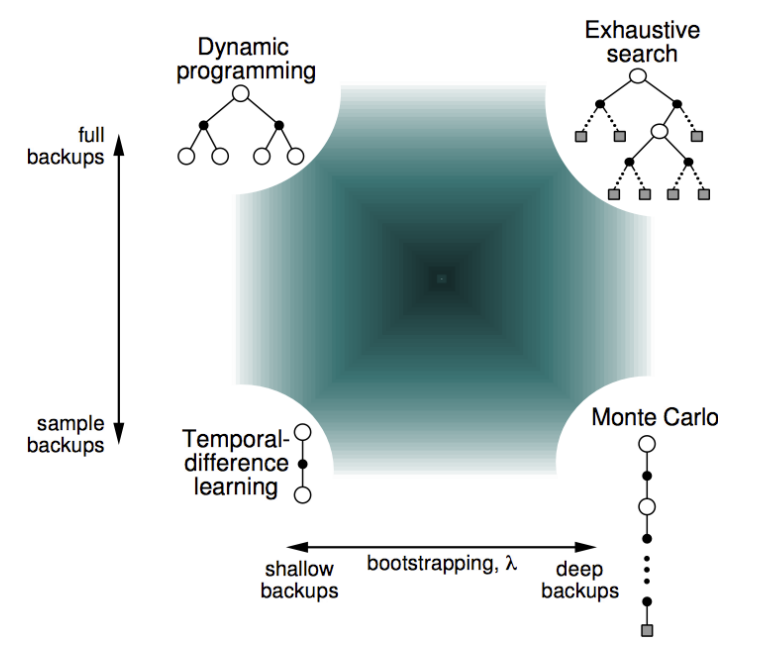
\includegraphics[width=0.68\textwidth]{rl_backup_space}
  \caption{Lo spazio dei metodi di apprendimento e pianificazione,
    classificati secondo la profondità dell'aggiornamento (asse
    orizzontale, superficiale a sinistra, profondo a destra) e la sua
    ampiezza (asse verticale, completo in alto, campionato in basso); le
    etichette in figura usano i termini inglesi \emph{shallow/deep
      backups} per l'asse orizzontale e \emph{full/sample backups} per il
    verticale. I quattro angoli corrispondono a dynamic programming,
    ricerca esaustiva, Temporal Difference e Monte Carlo. Adattata da
    \citet{suttonbarto2018}.}
  \label{fig:rl-backup-space}
\end{figure}

Le combinazioni dei due assi individuano quattro famiglie di metodi:

\begin{itemize}
  \item \textbf{Completo e superficiale}: la \emph{dynamic programming},
        che calcola l'aspettativa esatta su tutti i successori $s'$ ma si
        ferma dopo un solo passo, facendo bootstrapping sulla stima già
        disponibile del valore di $s'$ invece di espandere ulteriormente
        l'albero.
  \item \textbf{Completo e profondo}: la \emph{ricerca esaustiva}, che
        come la dynamic programming pesa ogni successore con la sua
        probabilità, ma che espande però l'intero
        albero delle conseguenze fino alla fine dell'episodio o a un
        orizzonte fissato. È il caso ideale in cui ci si potesse
        permettere di enumerare ogni possibile continuazione.
  \item \textbf{Campionato e profondo}: il \emph{Monte Carlo} non
        usa $P(s'\mid s,a)$, osserva un'unica traiettoria
        effettivamente realizzata e ne percorre per intero le conseguenze
        fino alla fine dell'episodio, calcolando il ritorno effettivo
        $G_t = \sum_k \gamma^k r_{t+k}$ senza mai usare bootstrapping.
  \item \textbf{Campionato e superficiale}: il \emph{Temporal
          Difference} (TD), che come Monte Carlo osserva una singola
        transizione campionata anziché un'aspettativa sul modello, ma
        come la dynamic programming si ferma dopo un solo passo,
        facendo bootstrapping sulla stima corrente del valore dello stato
        successivo.
\end{itemize}

Nella sua versione più semplice di Temporal Difference, TD(0),
l'aggiornamento della funzione valore-stato è
\[V(s_t) \leftarrow V(s_t) + \eta\big[(r_t + \gamma V(s_{t+1})) - V(s_t)\big],\]
dove il termine tra parentesi quadre è il \emph{Temporal Difference
  error}, ovvero la discrepanza tra la stima corrente e un target
calcolato guardando avanti di un solo passo. Il bootstrapping ha un costo,
l'errore della stima usata come target si propaga nell'aggiornamento, ma
un beneficio pratico decisivo rispetto a Monte Carlo: l'agente può
aggiornarsi a ogni singolo passo, senza attendere la fine dell'episodio,
un requisito essenziale per imparare da compiti molto lunghi o
addirittura privi di una fine naturale. Il Q-learning descritto di
seguito applica esattamente questo principio alla funzione valore-azione
$Q$ invece che alla sola funzione valore-stato $V$.

Questo lavoro si colloca nella casistica dell'aggiornamento campionato e superficiale, quello del Temporal Difference.
L'assenza di un modello della dinamica del traffico (§\ref{subsec:model-free}) esclude
già di per sé la dynamic programming e la ricerca esaustiva, entrambe
legate a un aggiornamento completo; inoltre la simulazione in \textsc{CityFlow} procede
per episodi lunghi e continui su intersezioni multiple, un contesto in
cui attendere la fine dell'episodio per ogni aggiornamento, come farebbe
Monte Carlo, sarebbe sia lento sia inutilmente rumoroso rispetto al
bootstrap a un passo. Il Q-learning e il DQN che ne deriva, discussi di
seguito, adottano infatti un aggiornamento TD, campionato e superficiale.

\subsection{Q-learning e Deep Q-Network}

\paragraph{Q-learning tabellare.} Il \textbf{Q-learning} \citep{suttonbarto2018} approssima $Q^*$
applicando iterativamente l'Equazione~\ref{eq:bellman-optimal} come
regola di aggiornamento tramite bootstrapping: a ogni transizione
osservata $(s,a,r,s')$, aggiusta il valore stimato $Q(s,a)$ verso il
target $r + \gamma \max_{a'} Q(s',a')$, la stima corrente al passo
successivo, invece di attendere il ritorno realizzato per intero a fine
episodio come farebbe un metodo Monte Carlo. Il nome "tabellare" indica
che questi aggiornamenti possono essere eseguiti considerando una tabella con una riga per ogni stato e una
colonna per ogni azione. L'aggiornamento modifica una voce alla volta e
ripetendo l'operazione su molte transizioni, ogni voce $Q(s,a)$ converge verso il
vero ritorno atteso dell'eseguire $a$ in $s$. Si ottiene in questo modo una politica
ottima, senza il bisogno di indicazioni esplicite sulle azioni da intraprendere.

L'approccio tabellare ha però un limite rappresentato dalle dimensioni della tabella.
Se lo spazio degli stati e lo spazio delle azioni sono continui o ad alta dimensionalità il numero di combinazioni possibili esplode,
rendendo questo approccio impraticabile.
Questo è il caso del controllo semaforico multi-agente, dove la dimensione dello spazio degli stati rende una
tabella esplicita irrealizzabile sia da costruire sia da aggiornare.

\paragraph{Deep Q-Network (DQN).} \citet{mnih2015dqn} risolvono il
problema sostituendo la tabella con una rete neurale $Q(s,a;\theta)$
allenata ad approssimarne i valori: invece di una voce indipendente per
ogni coppia $(s,a)$, la rete apprende una funzione continua che
generalizza a stati mai visti interpolando tra stati simili osservati
durante l'addestramento. I pesi $\theta$ vengono aggiornati
per discesa del gradiente in modo che $Q(s,a;\theta)$ si avvicini allo
stesso target di Bellman usato dal Q-learning tabellare, con la
differenza che l'aggiornamento modifica l'intera rete invece di una
singola voce, propagando l'informazione anche a stati simili mai
osservati direttamente. È esattamente questa proprietà a rendere il DQN
necessario in questo lavoro: lo spazio di stato del controllo semaforico
multi-agente è troppo grande per una tabella, ma una rete neurale può
generalizzare a partire da un numero gestibile di transizioni osservate
durante la simulazione. Gli autori introducono due accorgimenti per
stabilizzare questo schema, entrambi adottati anche in questo lavoro. Il
primo è il \emph{replay buffer}: una memoria in cui si accumulano le
transizioni $(s,a,r,s')$ osservate, da cui si campionano poi mini-batch
in ordine casuale per l'addestramento, rompendo la correlazione temporale
tra stati consecutivi di uno stesso episodio che violerebbe altrimenti
l'assunzione di campioni indipendenti richiesta dalla discesa del
gradiente stocastica. Come anticipato (§\ref{subsec:online-offline}), il
buffer non cambia la natura online del metodo, in quanto si riempie di
transizioni raccolte dalla politica corrente mentre l'addestramento
procede, non da un insieme fisso raccolto in anticipo. Il secondo è la
\emph{target network} $Q(\cdot;\theta^-)$, una copia dei pesi della rete
online sincronizzata solo periodicamente: calcolare il target $r +
  \gamma \max_{a'} Q(s',a';\theta^-)$ con questa copia invece che con la
rete online stessa, che cambia a ogni passo di gradiente, evita che il
bersaglio dell'ottimizzazione si sposti insieme ai pesi che lo
determinano, un problema noto come \emph{moving target}.

\subsection{Esplorazione $\varepsilon$-greedy}

Un agente completamente \emph{greedy}, che segue cioè sempre e solo l'azione a valore $Q$ stimato più
alto, non raccoglierebbe mai esperienza sulle conseguenze di azioni
alternative, rischiando di convergere su una politica sub-ottima per via
di una mancata esplorazione. Ad esempio, se nelle prime fasi
dell'addestramento un'azione appare leggermente migliore di un'altra, un
agente completamente \emph{greedy} la prediligerebbe sistematicamente,
impedendo di fatto all'agente di scoprire il potenziale di strategie alternative.
La tecnica più comune per bilanciare sfruttamento (\emph{exploitation}, scegliere
l'azione ritenuta migliore) ed esplorazione (\emph{exploration},
raccogliere informazione su azioni meno note) è $\varepsilon$-greedy
\citep{suttonbarto2018}: a
ogni passo di decisione, con probabilità $\varepsilon$ l'agente sceglie
un'azione uniformemente a caso, e con probabilità $1-\varepsilon$ sceglie
$\operatorname*{argmax}_a Q(s,a;\theta)$. Il valore di $\varepsilon$
tipicamente decresce nel corso dell'addestramento, da un valore iniziale
vicino a 1 (quasi solo esplorazione, quando la stima di $Q$ è ancora
inaffidabile) verso un valore finale piccolo ma non nullo (quasi solo
sfruttamento, mantenendo comunque un minimo di esplorazione residua).

\subsection{Estensioni usate in questo lavoro}

Il DQN di base ammette diverse estensioni indipendenti, ciascuna delle
quali corregge una specifica fonte di instabilità o inefficienza,
discusse di seguito:
\begin{itemize}
  \item Il \textbf{Double DQN} \citep{vanhasselt2016double} disaccoppia la
        selezione dell'azione dalla sua valutazione, usando la rete online per
        scegliere l'azione migliore e la target network, già introdotta sopra, solo
        per valutarla:
        $y = r + \gamma\, Q\!\left(s', \operatorname*{argmax}_{a'}
          Q(s',a';\theta);\ \theta^-\right)$. Poiché la stessa rete che sceglie
        l'azione con il valore stimato più alto tende anche a sovrastimarne il
        valore, usare la rete online per scegliere e la target network per
        valutare riduce questo bias sistematico di sovrastima tipico del DQN
        standard, che userebbe la stessa rete per entrambi i passi.
  \item Il \textbf{Prioritized Experience Replay} (PER,
        \citealp{schaul2016per}) sostituisce il campionamento uniforme dal
        replay buffer con un campionamento proporzionale al \emph{Temporal Difference error} $\delta_i$.
        Le transizioni che la rete predice peggio vengono ricampionate più
        spesso, concentrando la capacità di apprendimento dove serve di più.
        Assegnando a ciascuna transizione una priorità $p_i = |\delta_i| +
          \zeta$, con $\zeta$ una piccola costante che evita una probabilità
        nulla, la probabilità di campionamento è $P(i) = p_i^\alpha /
          \sum_k p_k^\alpha$, con $\alpha \in [0,1]$ iperparametro che ne
        controlla la dipendenza dall'errore. Per correggere il bias introdotto
        da un campionamento non uniforme, la loss viene pesata tramite
        coefficienti di \emph{importance sampling} $w_i = \left(N \cdot
          P(i)\right)^{-\beta}$, dove $N$ è la dimensione del buffer e $\beta \in
          [0,1]$ un iperparametro che cresce nel corso dell'addestramento verso
        1, aumentando progressivamente il grado di correzione applicato.
  \item La \textbf{Huber loss} (o \emph{smooth L1}) sostituisce la funzione di loss data dall'errore
        quadratico medio (MSE) con una funzione quadratica vicino allo zero e
        lineare lontano da esso, risultando meno sensibile agli outlier
        prodotti da transizioni con errore di stima molto grande (con MSE, un
        singolo errore enorme domina il gradiente dell'intero batch; con Huber
        il suo contributo cresce solo linearmente):
        \begin{equation}
          L_\kappa(y, \hat y) =
          \begin{cases}
            \tfrac{1}{2}(y-\hat y)^2                           & \text{se } |y-\hat y| \le \kappa \\
            \kappa\left(|y-\hat y| - \tfrac{1}{2}\kappa\right) & \text{altrimenti}
          \end{cases}
        \end{equation}
        Tipicamente $\kappa = 1$.
\end{itemize}

\subsection{Apprendimento multi-agente}
\label{subsec:marl}

Quanto descritto finora assume un solo agente che interagisce con
un solo ambiente. Quando più agenti operano nello stesso ambiente,
ciascuno osservando solo una porzione dello stato globale e influenzando
con le proprie azioni anche ciò che gli altri agenti osservano e
ricevono come ricompensa, il problema si generalizza da MDP a
\emph{processo decisionale di Markov decentralizzato e parzialmente
  osservabile} (Dec-POMDP). Il termine "decentralizzato" si riferisce al fatto che non esiste un'unica
azione scelta da un solo decisore, ma $N$ azioni scelte
indipendentemente da $N$ agenti; "parzialmente osservabile" indica invece che ogni
agente vede solo il proprio stato locale, non lo stato globale
completo dell'ambiente. Nel contesto di questo lavoro, la decentralizzazione si concretizza nel fatto che
ogni intersezione decide autonomamente la propria fase, mentre l'osservabilità
parziale si concretizza nel campo visivo limitato di ciascuna intersezione
(Capitolo~\ref{cap:tsc-modelli}), che esclude deliberatamente
dallo stato osservato ciò che accade agli altri incroci.

Il multi-agente introduce una difficoltà che il caso a singolo agente non
ha: la \emph{non stazionarietà}. L'equazione di Bellman e l'intera teoria
del Q-learning assumono che l'ambiente risponda in modo coerente nel
tempo alla stessa azione nello stesso stato; ma se più agenti apprendono
simultaneamente, ciascuno sta anche cambiando il proprio comportamento
mentre gli altri lo osservano, cosicché per ogni singolo agente
l'ambiente (che include il comportamento degli altri agenti) appare
cambiare regole nel tempo, anche se le vere dinamiche fisiche sottostanti
restano identiche.

Una seconda difficoltà è
l'\emph{assegnazione del merito} (\emph{credit assignment}), per la quale quando più
agenti contribuiscono a un solo risultato osservato, non è ovvio quale
frazione di quel risultato attribuire a ciascuno. Tale problema però non si pone se ogni agente riceve una ricompensa
calcolata esclusivamente sul proprio stato locale, così come avviene in questo lavoro.
Una versione attenuata resta comunque presente: lo stato locale di un agente, e
quindi la sua stessa ricompensa, dipende in parte dalle scelte degli altri agenti, per cui
l'effetto della propria azione e quello dell'azione altrui rimangono in
parte intrecciati anche con una ricompensa puramente locale.

Due schemi di coordinamento ricorrono in letteratura
\citep{li2018drlsurvey}: l'\emph{addestramento centralizzato con
  esecuzione decentralizzata} (CTDE), in cui gli agenti condividono
informazione globale solo durante il training per poi decidere
localmente, e l'\emph{addestramento ed esecuzione entrambi
  decentralizzati} (DTDE), in cui l'informazione resta sempre e solo
locale, anche durante l'addestramento. Una scelta indipendente da questa
è se i diversi agenti condividano o meno gli stessi pesi (\emph{parameter
  sharing}): condividerli riduce il numero di parametri totali e permette a
un agente di beneficiare dell'esperienza raccolta da tutti gli altri, a
costo di una minore capacità di specializzarsi su condizioni locali
peculiari, a meno che il meccanismo non trovi un altro modo per
differenziare il comportamento tra agenti pur condividendo i pesi.

Questo lavoro rappresenta un sistema multi-agente in cui ogni intersezione della
rete stradale è un agente a sé, con un proprio stato $s_i^t$, una propria
azione $a_i^t$ (la fase semaforica scelta) e una propria ricompensa
$r_i^t$, calcolati indipendentemente per ogni intersezione $i$
(Capitolo~\ref{cap:tsc-modelli}). L'architettura è di tipo DTDE, con scambio di
informazione locale tra intersezioni vicine (§\ref{sec:background-gnn}), e
adotta il parameter sharing: tutte le intersezioni condividono la stessa
rete $Q$, ma un meccanismo di meta-learning genera pesi diversi per nodi con caratteristiche locali diverse, così da
attenuare proprio il costo della condivisione appena descritto. Va
precisato che questa condivisione, insieme al fatto che l'aggiornamento
del gradiente sia calcolato in un solo passo che aggrega la loss di tutte
le intersezioni (Capitolo~\ref{cap:tsc-modelli}), non rende
l'addestramento centralizzato nel senso di CTDE: ciò che definisce quello
schema è l'uso, durante il solo training, di informazione non disponibile
in esecuzione, mentre qui ogni termine della loss usa esclusivamente lo
stato e la ricompensa locali della propria intersezione, esattamente gli
stessi disponibili in esecuzione.

Quando la rete $Q$ include un modulo ricorrente, condividere i pesi tra
le intersezioni pone un'ulteriore difficoltà legata allo stato ricorrente
campionato dal replay buffer, discussa in
§\ref{sec:background-rnn} dopo aver introdotto le reti ricorrenti.

\section{Reti Neurali Ricorrenti}
\label{sec:background-rnn}

Una rete neurale \emph{feedforward} calcola il proprio output come
funzione del solo input corrente. Dunque ogni esempio è trattato in modo
indipendente dai precedenti, e la rete non conserva alcuna memoria di
cosa abbia visto in passato. Questa assunzione fallisce ogni volta che i
dati hanno una struttura sequenziale in cui l'ordine e la storia contano
quanto il singolo valore osservato (testo, audio, serie temporali, o lo
stato di un'intersezione stradale). Le \emph{reti neurali ricorrenti} (RNN)
affrontano il problema introducendo un ciclo: a ogni istante $t$, un nodo
riceve in ingresso non solo il dato corrente $x^{t}$ ma anche il proprio
stato nascosto al passo precedente $h^{t-1}$,
\begin{equation}
  h^{t} = \sigma\!\left(W_{hx} x^{t} + W_{hh} h^{t-1} + b_h\right),
  \label{eq:rnn-recurrence}
\end{equation}
così che l'informazione rilevante di tutta la sequenza osservata fino a
$t$ possa, in linea di principio, persistere in $h^{t}$. Lo stesso
insieme di pesi $W_{hx}, W_{hh}, b_h$ viene riapplicato a ogni istante di
tempo, invece di avere pesi diversi per ogni passo. "Srotolando" la rete
lungo l'asse del tempo, cioè disegnando esplicitamente una copia dei nodi
per ogni istante $t=1,2,\dots$ collegata alla successiva (Figura~\ref{fig:rnn-unrolled}), ogni passo
diventa uno strato di una rete feedforward molto profonda a pesi
condivisi, addestrabile con la stessa backpropagation vista in precedenza
applicata lungo la sequenza anziché lungo i layer: questo algoritmo
prende il nome di \emph{backpropagation through time} (BPTT).

\begin{figure}[htbp]
  \centering
  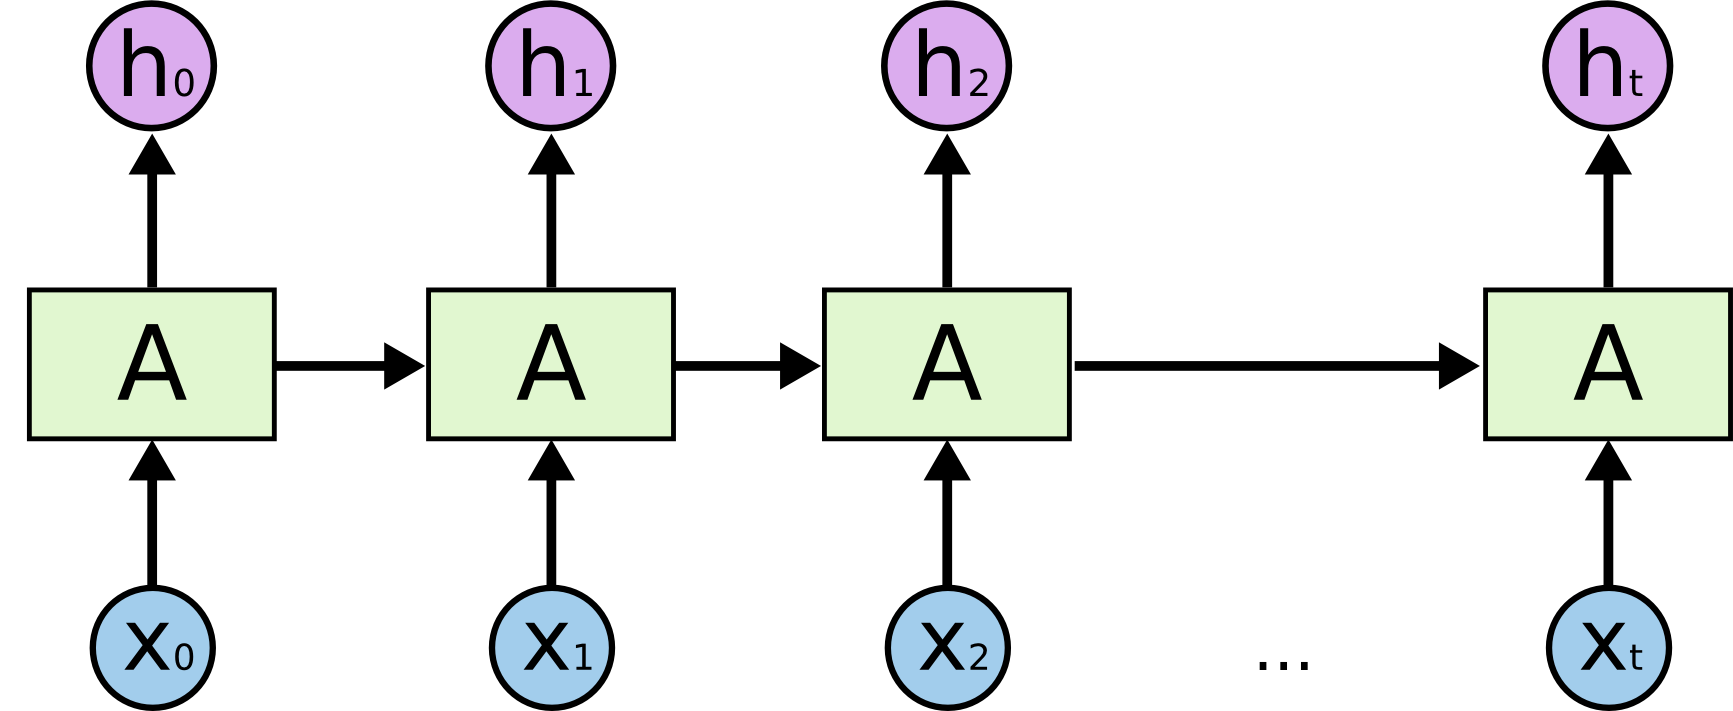
\includegraphics[width=0.75\textwidth]{rnn_unrolled}
  \caption[La rete ricorrente srotolata lungo il tempo.]{La rete ricorrente srotolata lungo il tempo: il modulo $A$
    rappresenta la funzione ricorrente, ad esempio l'Equazione~\ref{eq:rnn-recurrence},
    riapplicata con gli stessi pesi a ogni istante. Fonte: adattata da
    una discussione su Stack
    Exchange.\footnote{\url{https://stats.stackexchange.com/questions/341085/keras-difference-between-gru-and-grucell}}}
  \label{fig:rnn-unrolled}
\end{figure}

\paragraph{Il problema del gradiente.} Una rete ricorrente addestrata su
sequenze lunghe soffre di un problema strutturale: il gradiente
propagato all'indietro attraverso molti passi temporali tende ad annullarsi
(\emph{vanishing gradient}) o a divergere (\emph{exploding gradient}) a
seconda che i pesi ricorrenti abbiano modulo minore o maggiore di uno,
poiché il gradiente si ottiene moltiplicando ripetutamente per lo stesso
fattore a ogni passo srotolato, esattamente come una potenza $c^n$ tende a
zero o esplode al crescere di $n$ a seconda che $|c|$ sia minore o
maggiore di uno. Nella pratica, questo rende di fatto impossibile
apprendere dipendenze che coprono più di poche decine di passi con una
RNN semplice.

\paragraph{Long Short-Term Memory (LSTM).}
L'LSTM \citep{hochreiter1997lstm, lipton2015rnnreview}
risolve il problema sostituendo il semplice nodo ricorrente con una
\emph{cella di memoria}: uno stato interno $c^{t}$ collegato a se stesso
da un percorso a peso fisso unitario (il \emph{constant error carousel}),
attraverso cui il gradiente può fluire per molti passi senza annullarsi né
esplodere. L'accesso a questo stato è
regolato da tre \emph{gate}, unità sigmoidali il cui valore in $[0,1]$
modula quanta informazione passi attraverso di esse (Figura~\ref{fig:lstm-cell}).

\begin{figure}[htbp]
  \centering
  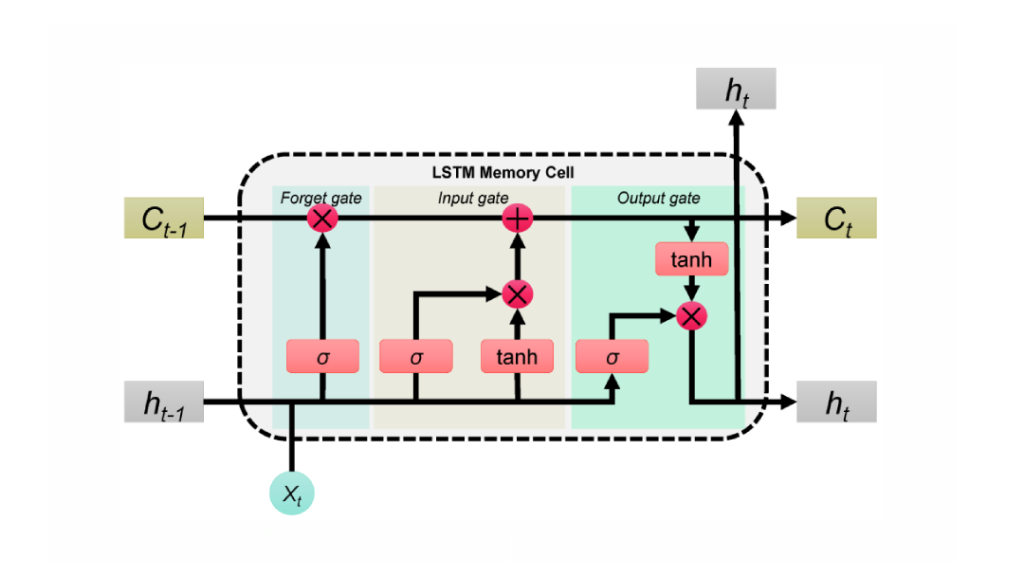
\includegraphics[width=0.7\textwidth]{lstm_cell}
  \caption[La cella di memoria dell'LSTM.]{La cella di memoria dell'LSTM: il forget gate decide quanto
    dello stato precedente mantenere, l'input gate quanto del nuovo
    contenuto candidato incorporare, l'output gate quanto dello stato
    risultante esporre come output. Fonte: adattata da
    dida.do.\footnote{\url{https://dida.do/what-is-an-lstm-neural-network}}}
  \label{fig:lstm-cell}
\end{figure}

A livello formale, con pesi $W_g \in \mathbb{R}^{2d_1 \times d_1}$ e bias $b_g \in
  \mathbb{R}^{d_1}$ condivisi da ogni nodo, i tre gate e il contenuto
candidato $g \in \{\text{forget, input, output, cell}\}$ si calcolano
come:
\begin{equation}
  \begin{bmatrix} f^t \\ \iota^t \\ o^t \\ g^t \end{bmatrix} =
  \begin{bmatrix} \sigma \\ \sigma \\ \sigma \\ \tanh \end{bmatrix}
  \left(
  W_{\{f,\iota,o,g\}}^{\top} [\,x^t \,\|\, h^{t-1}\,] + b_{\{f,\iota,o,g\}}
  \right),
  \label{eq:lstm-background-gates}
\end{equation}
\[ c^t = f^t \odot c^{t-1} + \iota^t \odot g^t, \]
\[ h^t = o^t \odot \tanh(c^t); \]
il \emph{forget gate} $f$ decide quanto dello stato precedente
dimenticare, l'\emph{input gate} $\iota$ quanto del nuovo contenuto
candidato $g$ incorporare
nello stato aggiornato, e l'\emph{output gate} $o$ quanto dello stato
risultante esporre come output della cella. Il contenuto candidato $g$
non è esso stesso un gate, cioè un moltiplicatore in $[0,1]$, ma il nuovo
valore, calcolato con $\tanh$ e quindi in $[-1,1]$, che i gate regolano.
Un valore di forget gate
vicino a 1 lascia passare l'informazione pregressa quasi inalterata anche
dopo molti passi; uno vicino a 0 la cancella, permettendo alla rete di
"dimenticare" deliberatamente informazione non più rilevante.

\paragraph{Gated Recurrent Unit (GRU).} Una variante più leggera dell'LSTM,
la \textbf{GRU} \citep{cho2014gru}, fonde il \emph{forget gate} e
l'\emph{input gate} in un unico \emph{update gate} e rinuncia allo stato di
cella $c^{t}$ separato, esponendo un solo stato nascosto $h^{t}$ sia
come memoria interna sia come output. Si hanno così meno parametri da addestrare e un
grafo computazionale più semplice, a fronte di una capacità di
rappresentazione leggermente inferiore rispetto ai quattro gate distinti
dell'LSTM. Le due varianti raggiungono nella pratica prestazioni simili su
molti compiti, e la scelta tra loro è spesso guidata più dalla
convenzione di un'architettura di riferimento che da un vantaggio netto
dell'una sull'altra: questo lavoro adotta l'LSTM per coerenza con il
modello di riferimento \citep{wang2022metastgat}.

\paragraph{Replay ricorrente e disallineamento dello stato.} Quando la
rete $Q$ include un modulo ricorrente come l'LSTM appena descritto,
campionare dal replay buffer (§\ref{sec:background-rl}) transizioni
isolate anziché intere sequenze pone un problema specifico: lo stato
ricorrente $(h,c)$ usato durante l'addestramento non coincide
necessariamente con quello osservato durante la raccolta dati. Per una
transizione campionata isolatamente, l'unica scelta praticabile è
inizializzare $(h,c)$ a zero, un disallineamento rispetto allo stato che
la rete aveva effettivamente accumulato in quel punto della sequenza
originale, un problema noto come \emph{hidden state staleness}. Seguendo
\citet{kapturowski2019r2d2} (R2D2), il campionamento si esegue allora su
intere sequenze di lunghezza $L$, dedicando i primi passi della sequenza
(fase di \emph{burn-in}) esclusivamente alla ricostruzione di uno stato
ricorrente plausibile, senza calcolare gradiente, per poi eseguire la
BPTT sui passi restanti.

\section{Grafi e Graph Neural Network}
\label{sec:background-gnn}

\subsection{Cos'è un grafo}

Un \emph{grafo} $G = (V, E)$ è una struttura matematica composta da un
insieme di \emph{nodi} $V$ e un insieme di \emph{archi}
$E$, dove ogni arco collega una coppia di nodi. È lo strumento standard
per rappresentare entità e le relazioni tra loro, quando quelle relazioni
non hanno una struttura regolare o sequenziale. Ne sono esempi una rete di amicizie tra
persone, le pagine web collegate da link, le molecole i cui atomi sono
legati da legami chimici, e, in questo lavoro, una rete stradale, dove i
nodi sono le intersezioni e gli archi le strade che le collegano
direttamente.

Un arco può essere \emph{diretto} (se indica un verso) o \emph{non diretto} (se indica una relazione simmetrica, Figura~\ref{fig:graph-directed});
può inoltre avere un \emph{peso} associato, un numero che quantifica l'intensità o il costo della relazione.

\begin{figure}[htbp]
  \centering
  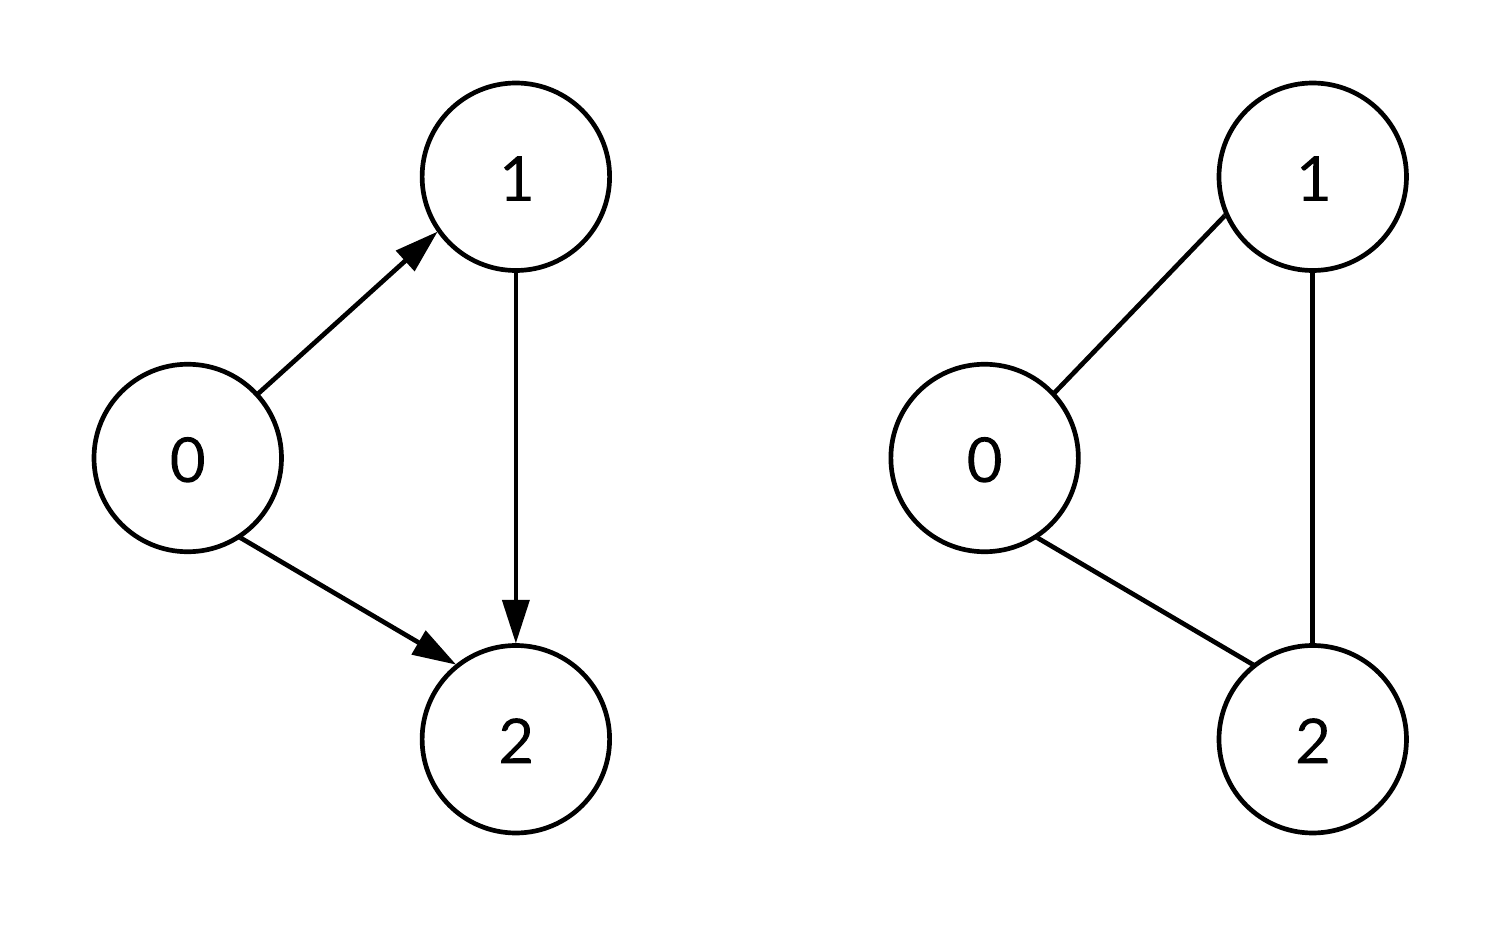
\includegraphics[width=0.75\textwidth]{graph_directed_undirected}
  \caption{Esempi di grafo diretto (sinistra) e non diretto (destra).}
  \label{fig:graph-directed}
\end{figure}

L'insieme dei nodi
collegati a un nodo $i$ tramite un arco si chiama
\emph{vicinato} di $i$, indicato $\mathcal{N}(i)$; il numero di archi
incidenti su $i$ è il suo \emph{grado}. Una sequenza di nodi collegati
uno al successivo da un arco è un \emph{cammino}; la lunghezza del
cammino più breve tra due nodi qualunque è la loro \emph{distanza} sul
grafo, misurata in numero di archi. Un grafo con $N$ nodi si può
rappresentare in forma matriciale con la \emph{matrice di adiacenza} $A
  \in \{0,1\}^{N \times N}$, dove $A_{iu}=1$ se e solo se esiste un arco tra
$i$ e $u$ (o il peso dell'arco, se il grafo è pesato, invece del semplice
$1$). È spesso utile
aggiungere a ogni nodo un \emph{self-loop}, un arco da un nodo verso se
stesso ($A_{ii}=1$), cosicché un nodo sia incluso nel proprio stesso
vicinato: la notazione $\hat A = A + I$ indica questa aggiunta e ricorre
nelle equazioni seguenti.

Un piccolo esempio: la matrice di adiacenza senza pesi del grafo non diretto in Figura~\ref{fig:graph-directed} è data da
\[A = \begin{pmatrix} 0&1&1 \\ 1&0&1 \\ 1&1&0 \end{pmatrix}.\]
Con l'aggiunta dei self-loop, $\hat A = A+I$ ha inoltre un $1$ su ogni elemento della diagonale.

Nella rete stradale di questo lavoro, ogni nodo $i$ del grafo porta con sé
un vettore di caratteristiche (o \emph{embedding}) che ne descrive lo
stato corrente, ad esempio quanti veicoli attendono su ciascuna corsia.
Il problema che le \emph{graph neural network} risolvono è come far sì che l'embedding di un nodo
tenga conto anche di ciò che accade nei nodi a lui collegati, non solo del proprio stato isolato.

\subsection{Message passing}

Le \emph{Graph Neural Network} (GNN) affrontano questo problema con un
principio comune, il \emph{message passing} \citep{wu2021gnnsurvey,
  bacciu2020gentlegnn}. A ogni iterazione (o \emph{layer}) $l$, ogni nodo
$i$ con rappresentazione corrente $h_i^{(l)}$ esegue due operazioni in
successione: prima un passo di \emph{aggregazione}, che combina i
messaggi ricevuti da ciascun vicino $u \in \mathcal{N}(i)$ in un unico
vettore di messaggio $m_i$,
\[m_i = \mathrm{AGGREGATE}\big(\{h_u^{(l)} : u \in \mathcal{N}(i)\}\big),\]
poi un passo di \emph{aggiornamento}, che combina il messaggio
aggregato con la rappresentazione precedente dello stesso nodo per
produrre quella nuova,
\[h_i^{(l+1)} = \mathrm{UPDATE}\big(h_i^{(l)},\ m_i\big).\]
Tutte le GNN discusse in questa tesi, incluse le formulazioni di
seguito, sono istanze di questo stesso schema generale, mostrato in
Figura~\ref{fig:gnn-pipeline}, che differiscono
solo nella scelta concreta di AGGREGATE e UPDATE. Nella GCN, AGGREGATE è
una media pesata dalla sola topologia; nella GAT, un peso appreso in base
al contenuto dei due nodi coinvolti. Impilando più layer, l'informazione
può viaggiare oltre il solo vicinato immediato: dopo $k$ layer, la
rappresentazione di un nodo dipende (indirettamente) da tutti i nodi
raggiungibili entro $k$ archi di distanza, poiché il messaggio ricevuto da
un vicino al layer $l$ incorpora già, ricorsivamente, i messaggi che
quel vicino aveva ricevuto dai propri stessi vicini al layer $l-1$.

\begin{figure}[htbp]
  \centering
  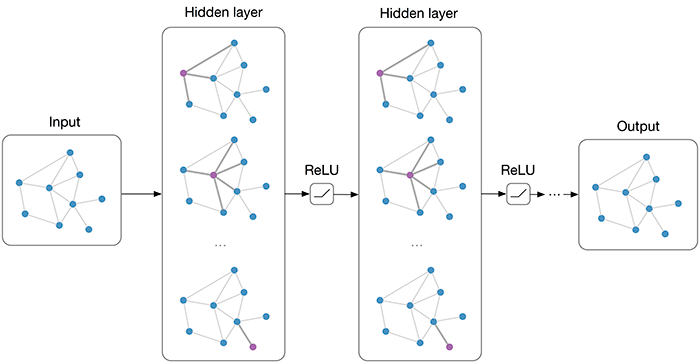
\includegraphics[width=0.85\textwidth]{gnn_pipeline}
  \caption[Lo schema generale di message passing impilato su più layer.]{Lo schema generale di message passing impilato su più layer: a
    ogni layer ciascun nodo aggrega le rappresentazioni
    dei propri vicini e aggiorna la propria, prima di applicare la non
    linearità $\sigma$ e passare al layer successivo. Fonte: adattata da
    Towards
    AI.\footnote{\url{https://pub.towardsai.net/graph-attention-networks-paper-explained-with-illustration-and-pytorch-implementation-eb35edba562c}}}
  \label{fig:gnn-pipeline}
\end{figure}

\paragraph{Graph Convolutional Network (GCN).} \citet{kipf2017gcn}
propongono la formulazione più basilare di message passing tra quelle qui
discusse. La rappresentazione di ciascun nodo si aggiorna mediando quelle
dei vicini con un peso fisso, determinato unicamente dalla topologia
locale (quanti vicini ha un nodo), non dal contenuto delle
rappresentazioni stesse. Indicando con $\hat A = A + I$ la matrice di
adiacenza con self-loop e con $\hat D$ la matrice diagonale dei gradi
corrispondente ($\hat D_{ii} = \sum_u \hat A_{iu}$), la regola di
propagazione di un singolo layer si scrive, in forma matriciale:
\begin{equation}
  H^{(l+1)} = \sigma\!\left(\hat D^{-1/2} \hat A\, \hat D^{-1/2} H^{(l)} W^{(l)}\right)
  \label{eq:gcn-propagation}
\end{equation}
dove $H^{(l)} \in \mathbb{R}^{N \times d_l}$ raccoglie le rappresentazioni
di tutti gli $N$ nodi del grafo al layer $l$, $W^{(l)}$ è la matrice di
pesi condivisa da ogni nodo e $\sigma$ una non linearità puntuale. Per un
singolo nodo $i$, la normalizzazione simmetrica $\hat D^{-1/2}\hat
  A\hat D^{-1/2}$ equivale a pesare il contributo di ogni vicino $u$ con
$1/\sqrt{\hat d_i \hat d_u}$:
\begin{equation}
  h_i^{(l+1)} = \sigma\!\left(\sum_{u \in \mathcal{N}(i) \cup \{i\}}
  \frac{1}{\sqrt{\hat d_i \hat d_u}}\, W^{(l)} h_u^{(l)}\right)
  \label{eq:gcn-aggregate}
\end{equation}
un peso identico per ogni arco del vicinato di $i$, funzione solo del
grado dei due nodi coinvolti e mai del loro contenuto. È, per costruzione,
il termine di paragone più naturale rispetto a cui misurare cosa aggiunge
un meccanismo di attenzione appreso come quello discusso di seguito.

\paragraph{Graph Attention Network (GAT).} \citet{velickovic2018gat}
sostituiscono il peso fisso della GCN con un coefficiente di attenzione
appreso, specifico per ciascuna coppia di nodi collegati: il contributo di
un vicino non dipende più soltanto dalla topologia, ma anche dal suo
contenuto. Dato un nodo $i$ con vicinato $\mathcal{N}(i)$, embedding di
input $h_i$, matrice di proiezione condivisa $W$ e vettore di attenzione
$\vec a$:
\begin{equation}
  e_{iu} = \mathrm{LeakyReLU}\!\left(\vec a^\top [W h_i \,\|\, W h_u]\right),
  \qquad
  \alpha_{iu} = \frac{\exp(e_{iu})}{\sum_{u' \in \mathcal{N}(i)} \exp(e_{iu'})}
  \label{eq:gat-attention}
\end{equation}
\begin{equation}
  h_i' = \sigma\!\left(\sum_{u \in \mathcal{N}(i)} \alpha_{iu}\, W h_u\right)
  \label{eq:gat-aggregate}
\end{equation}
dove $\|$ denota la concatenazione: $e_{iu}$ è un punteggio di
compatibilità grezzo tra $i$ e $u$, che il \emph{softmax} sul vicinato
trasforma in un coefficiente $\alpha_{iu} \in [0,1]$ che somma a uno su
tutti i vicini di $i$, esattamente come una distribuzione di probabilità,
come illustrato in Figura~\ref{fig:gat-attention}.

\begin{figure}[htbp]
  \centering
  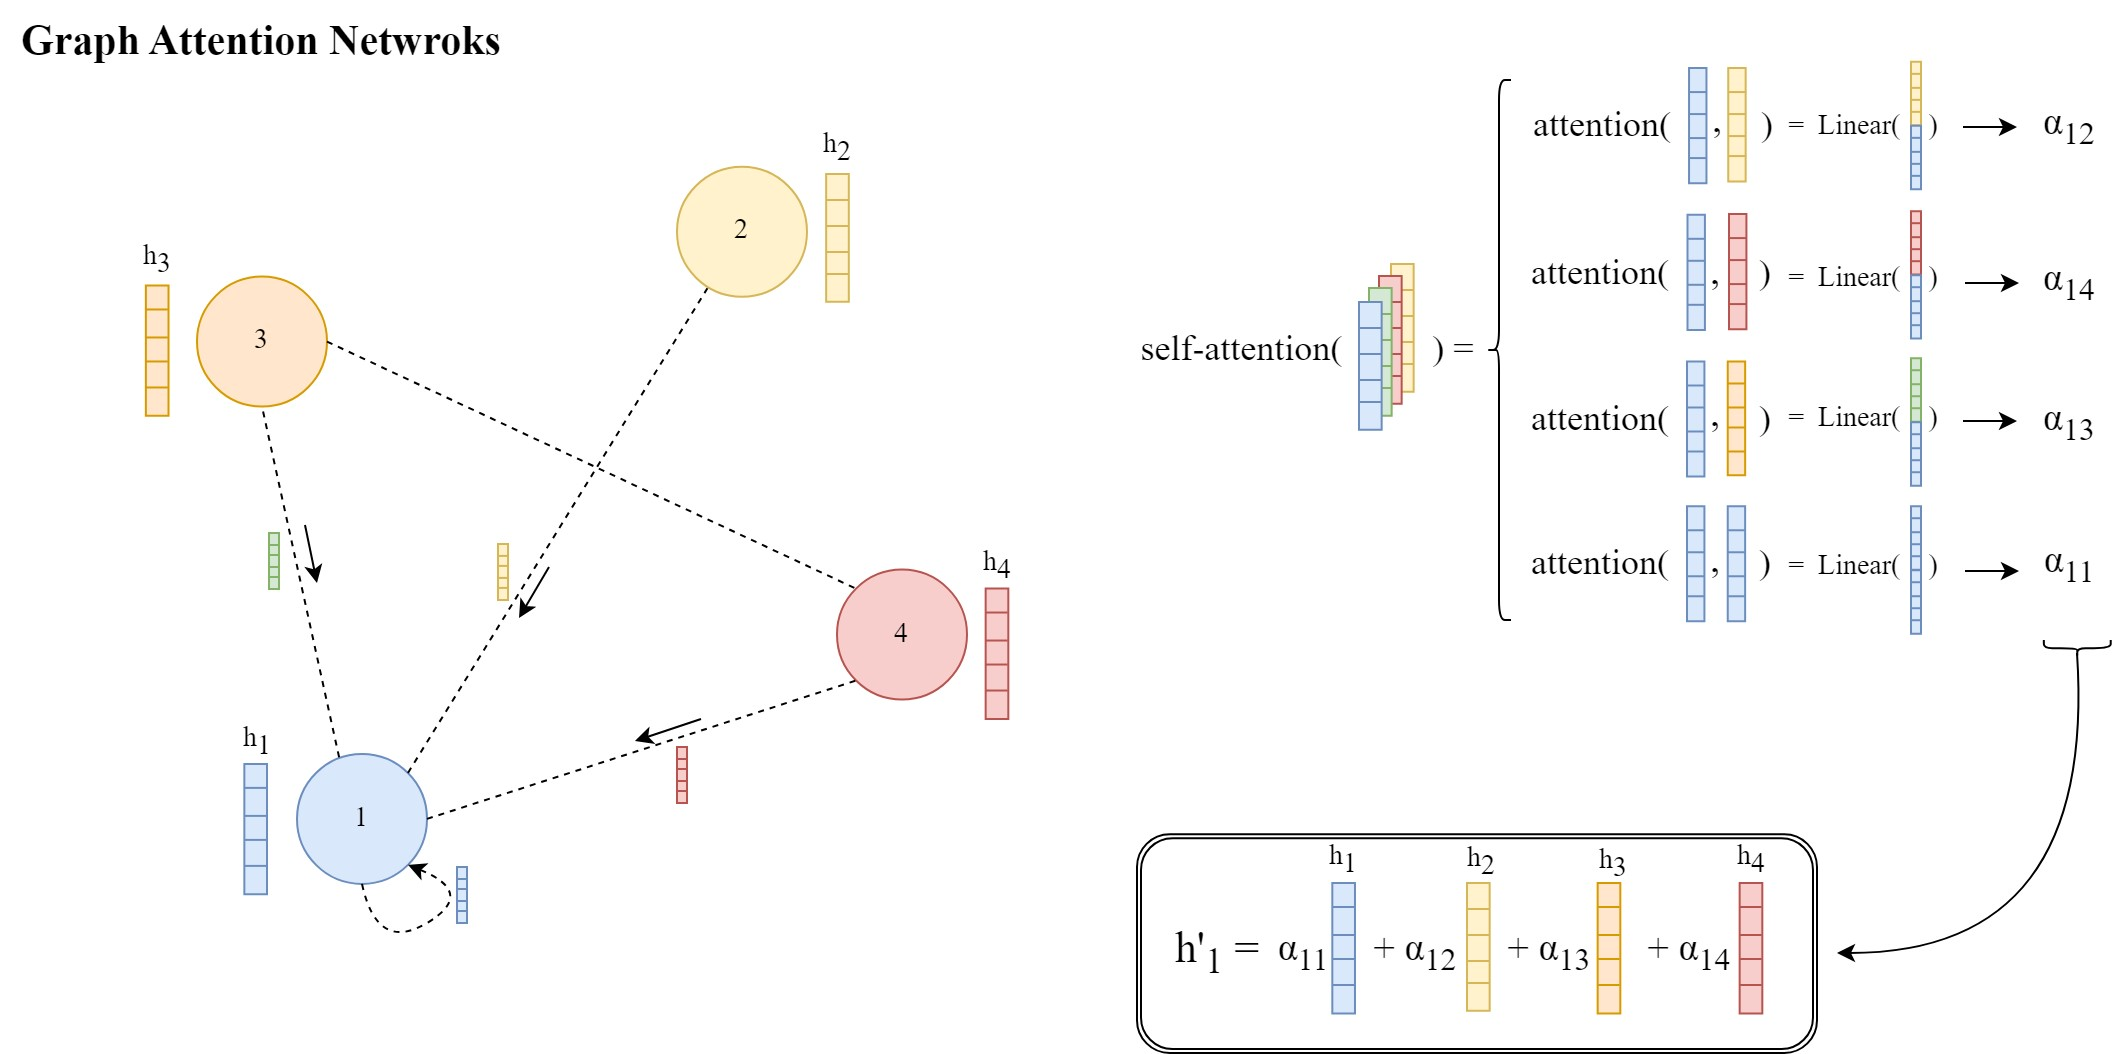
\includegraphics[width=0.95\textwidth]{gat_attention}
  \caption[Il calcolo dell'attenzione per il nodo 1 rispetto al proprio vicinato.]{Il calcolo dell'attenzione per il nodo $1$ rispetto al proprio
    vicinato $\{1,2,3,4\}$ (con self-loop incluso): ogni coppia
    $(h_1,h_u)$ produce un coefficiente $\alpha_{1u}$, usato poi per
    combinare linearmente gli embedding dei vicini nella nuova
    rappresentazione $h_1'$. La figura, semplificata a scopo illustrativo,
    accorpa in un unico passo "Linear" il calcolo di compatibilità e la
    normalizzazione softmax descritti nel testo, e omette la proiezione
    condivisa $W$ e la non linearità $\sigma$. Fonte: adattata da Data
    Science at
    Home.\footnote{\url{https://datascienceathome.com/the-power-of-graph-neural-networks-understanding-the-future-of-ai-part-2-2-ep-224/}}}
  \label{fig:gat-attention}
\end{figure}

Con $K$ teste di attenzione indipendenti (\emph{multi-head attention}),
ciascuna con i propri pesi $W$ e $\vec a$, gli output si concatenano nei
layer intermedi e si mediano nell'ultimo, secondo lo schema introdotto per
l'attenzione da \citet{vaswani2017attention}. In questo modo teste diverse possono
imparare a specializzarsi su aspetti diversi della relazione tra due nodi.
A differenza della GCN, il coefficiente $\alpha_{iu}$ consente a un nodo
di ponderare diversamente i propri vicini in base al loro contenuto, non
solo alla loro posizione nel grafo: una proprietà rilevante per
un nodo i cui vicini abbiano importanza marcatamente diversa,
come nel caso di un incrocio stradale in cui passano un'arteria principale e una strada
secondaria. La funzione di compatibilità additiva appena descritta, per
quanto la più nota, non è l'unica possibile: il Capitolo~\ref{cap:tsc-modelli}
(Meta-GAT) ne impiega una variante strutturalmente diversa, con Query, Key
e Value esplicite e distinte al posto della proiezione $W$ condivisa, e un
prodotto scalare al posto della concatenazione.

\subsection{Invarianza ed equivarianza per permutazione}
\label{subsec:permutation-invariance}

Sia l'aggregazione della GCN sia quella della GAT condividono due
proprietà distinte, che vale la pena separare.

La prima è ciò che permette a queste reti di funzionare su grafi di
dimensione diversa senza dover riaddestrare nulla: i pesi $W$ sono
condivisi da ogni nodo, e l'operatore AGGREGATE (una somma pesata, sia
essa uniforme come nella GCN o per attenzione come nella GAT) accetta un
numero qualsiasi di vicini. Il numero di parametri del layer non dipende
quindi dal numero di nodi $N$ del grafo, una condizione necessaria perché
lo stesso modello, addestrato su un grafo di una certa dimensione, possa
essere applicato a un grafo di dimensione diversa.

La seconda è l'\emph{invarianza per permutazione} dell'operatore di
aggregazione: una somma non dipende dall'ordine in cui i suoi addendi
vengono elencati, quindi il messaggio aggregato $m_i$ di un nodo $i$ non
dipende dall'ordine in cui i vicini di $i$ vengono numerati o elencati,
ma solo da quali essi siano. È ciò che distingue strutturalmente una GNN
da una rete feedforward applicata a un vettore di caratteristiche di
lunghezza fissa. Una MLP a cui si desse in input, in un
qualche ordine arbitrario, le caratteristiche di ciascun nodo del grafo
concatenate assegnerebbe implicitamente un significato specifico a ciascuna
posizione del vettore (il primo blocco di ingressi, il secondo, ...) e
produrrebbe quindi un output diverso se semplicemente si rinumerassero i
nodi, pur descrivendo esattamente la stessa rete stradale.
\citet{wei2019colight} osservano esattamente questo limite per gli schemi
di coordinamento basati su una lista ordinata di vicini.

Applicando l'invarianza per permutazione a ogni nodo del grafo
simultaneamente, l'intero layer di message passing risulta
\emph{equivariante per permutazione}: rinumerare i nodi in ingresso
rinumera allo stesso modo le rappresentazioni prodotte in uscita, invece
di produrre un risultato arbitrariamente diverso
\citep{bronstein2021geometric}. È questa equivarianza, insieme
all'indipendenza del numero di parametri da $N$, a rendere possibile la
generalizzazione a topologie di rete mai viste che il
Capitolo~\ref{cap:confronto} conduce su MetaSTGAT e sulle sue varianti.

\subsection{Reti spatio-temporali su grafo}

Molti grafi non sono statici: la topologia resta fissa, ma le
caratteristiche osservate a ciascun nodo evolvono nel tempo, e le due
dimensioni, spaziale e temporale, risultano intrecciate, poiché il valore
osservato a un nodo in un dato istante è correlato sia con i valori
passati allo stesso nodo sia con quelli ai nodi limitrofi. La famiglia di modelli che combina un layer
di propagazione sul grafo (GCN o GAT, appena visti) con una componente
ricorrente (LSTM, §\ref{sec:background-rnn}) sull'asse temporale prende il
nome di \emph{spatiotemporal graph neural network} (STGNN), un termine
ormai consolidato nella letteratura sul forecasting di serie temporali
multivariate correlate \citep{cini2025graphdl}. MetaSTGAT, descritto nel
dettaglio nel Capitolo~\ref{cap:tsc-modelli}, costituisce un esempio di
questa famiglia applicata al controllo semaforico anziché alla previsione:
un layer di \emph{graph attention} cattura la dipendenza spaziale tra
intersezioni limitrofe, un layer ricorrente (LSTM) ne cattura l'evoluzione
temporale, e i due vengono addestrati congiuntamente end-to-end.

\subsection{Pesi generati da meta-learning}

Le strutture neurali introdotte, GCN e GAT, nella loro formulazione originale, condividono gli
stessi pesi su tutti i nodi del grafo: un'assunzione ragionevole
quando i nodi sono sufficientemente omogenei, meno quando, come in una
rete stradale reale, la topologia locale di ciascun nodo (numero di
strade entranti, presenza di un'arteria, posizione periferica o centrale)
può differire sensibilmente da nodo a nodo.
Un \emph{hypernetwork} \citep{ha2016hypernetworks} affronta il problema
generando i pesi di un layer non come parametri
fissi appresi direttamente, bensì come output di una seconda rete,
condizionata sulle caratteristiche locali del nodo: è di fatto una via di
mezzo tra pesi completamente condivisi e pesi completamente indipendenti
per ogni nodo, che riduce il costo del parameter sharing senza rinunciare
del tutto ai suoi benefici. Nel contesto di questo lavoro, un hypernetwork
condizionato su caratteristiche locali dell'intersezione è esattamente il
meccanismo che la letteratura sul controllo semaforico chiama
\emph{meta-learning} quando applicato a questo compito: i due termini
descrivono lo stesso principio, il secondo è quello più diffuso nei
lavori discussi in §\ref{sec:background-tsc}, dove si colloca
esplicitamente MetaSTGAT.

\subsection{Propagazione a lungo raggio}

Sia la GCN sia la GAT propagano informazione a un solo passo di distanza
(un arco nel grafo) per layer: raggiungere un vicino a distanza $k$
richiede impilarne altrettanti, con un costo di parametri crescente e un
rischio noto di \emph{over-smoothing} \citep{li2018oversmoothing}, per il quale le rappresentazioni
dei nodi divengono troppo omogenee al crescere della profondità (ogni nodo
finisce per "vedere" praticamente tutto il grafo, perdendo la capacità di
distinguersi dai propri vicini). Meccanismi più recenti, tra cui \textbf{SONAR} \citep{trenta2025sonar},
affrontano il problema della propagazione a lungo raggio secondo un
principio diverso, ispirato ai sistemi dinamici oscillatori piuttosto che
alla concatenazione sequenziale di layer. Il sistema si comporta come una
rete di masse collegate da molle e smorzatori, una massa per nodo del
grafo. Raccolto lo stato di tutti gli $N$ nodi al tempo continuo $t$ in
$X(t) \in \mathbb{R}^{N \times d}$, la sua evoluzione è governata da
un'equazione del second'ordine, un'accelerazione e non una semplice
velocità:
\begin{equation}
  \ddot X(t) = -\mathcal{L}^a X(t)\, W - D(X(t)) \odot \dot X(t) + F(X(t))
  \label{eq:sonar-wave-background}
\end{equation}
Tre termini, tre ruoli distinti. $\mathcal{L}^a$ è un Laplaciano di grafo
pesato da una conduttanza $a_{ui} \geq 0$ per arco, che tira lo stato di un
nodo verso quello dei suoi vicini $u \in \mathcal{N}(i)$, come una molla.
$D(\cdot) \geq 0$ è un termine dissipativo che agisce sulla velocità
$\dot X(t)$, frenando il movimento come un attrito. $F(\cdot)$ è una
forzante esterna, che inietta energia dall'esterno del sistema. Riscritta
come sistema del prim'ordine, con velocità ausiliaria $V=\dot X$, e
discretizzata con passo $h$ su $L$ iterazioni, l'aggiornamento a ogni
iterazione diventa:
\begin{equation}
  \begin{aligned}
    \big(\mathcal{L}^a X\big)_i & = \sum_{u \in \mathcal{N}(i)} a_{ui}\,(X_i - X_u),              \\
    V                           & \leftarrow V - h\big(\mathcal{L}^a X + D(X)\odot V - F(X)\big), \\
    X                           & \leftarrow X + h\,\tanh(V)
  \end{aligned}
  \label{eq:sonar-discrete-background}
\end{equation}
Le $L$ iterazioni condividono sempre gli stessi pesi $a_{ui}$, $D(\cdot)$ e
$F(\cdot)$, per cui, a differenza di uno stack di $L$ layer indipendenti
come GCN o GAT, il costo di parametri di questo meccanismo resta costante
al crescere di $L$, un vantaggio strutturale dichiarato dagli stessi
autori.

\section{Traffic Signal Control come problema}
\label{sec:background-tsc}

\subsection{Terminologia e metriche}
\label{subsec:tsc-terminologia}

Il \emph{traffic signal control} (TSC), o controllo semaforico, decide
periodicamente quali flussi veicolari autorizzare a un incrocio. Il
vocabolario di base, comune a questo capitolo e ai
Capitoli~\ref{cap:tsc-modelli} e~\ref{cap:confronto}, è il seguente.

Ogni via che affluisce a un incrocio è divisa in \emph{corsie}, ciascuna
tipicamente dedicata a una o più svolte (diritto, sinistra, destra). Un
\emph{movimento} è una coppia ordinata di corsie, una in ingresso e una
in uscita, che un veicolo può percorrere attraversando l'incrocio; una
\emph{fase} semaforica autorizza simultaneamente un sottoinsieme di
movimenti compatibili tra loro, cioè le cui traiettorie non si
intersecano. Il controllore osserva lo stato dell'incrocio e sceglie una
fase a ogni \emph{step di decisione}, un intervallo di tempo fissato che
si ripete per l'intera durata della simulazione.

Valutare un controllore richiede di misurare cosa succede ai veicoli. Il
\emph{tempo di percorrenza} (\emph{travel time}) di un veicolo è il tempo
trascorso tra il suo ingresso e la sua uscita dalla rete; l'\emph{attesa}
di un veicolo, in un dato istante, è il tempo per cui si trova fermo o
comunque non ancora oltre l'incrocio a cui si sta avvicinando. Il
\emph{throughput} di un incrocio o di una rete è invece il numero di
veicoli che riescono ad attraversarli nell'unità di tempo, una nozione
teorica distinta dalla percentuale di veicoli che completano
effettivamente il proprio percorso in una simulazione di durata finita,
misurata nel Capitolo~\ref{cap:confronto}. Le definizioni precise di
queste grandezze, e le metriche che questo lavoro ne ricava, sono
rimandate ai Capitoli~\ref{cap:tsc-modelli} e~\ref{cap:confronto}, dove
vengono usate per la prima volta in forma quantitativa.

\subsection{Due generazioni di controllo}
\label{subsec:tsc-generations}

Il TSC si articola in due approcci, in ordine crescente di complessità e,
storicamente, di introduzione \citep{shams2018atsctaxonomy}.

\textbf{Controllo a tempi fissi.} Un piano semaforico ciclico ripete
all'infinito la stessa sequenza di fasi, ciascuna di durata prestabilita
in base a stime di traffico medie e mai più rivista in tempo reale; nella
sua forma più diffusa nei sistemi reali, la ripartizione del verde tra le
fasi e la durata complessiva del ciclo possono variare per fascia
oraria, ma restano fissate a tavolino e non rispondono al traffico
osservato istante per istante. \textsc{Fixed-Time}, la baseline di questo
lavoro (Capitolo~\ref{cap:tsc-modelli}), ne è la forma più semplice:
cicla le fasi in ordine fisso, cambiando fase a ogni step di decisione,
senza alcun parametro da configurare oltre all'ordine del ciclo. È
estremamente semplice da implementare ed è tuttora la spina dorsale di
gran parte dei sistemi semaforici reali: negli Stati Uniti, ad esempio, una
larga proporzione delle intersezioni semaforizzate resta priva di sensori
di rilevamento ed è tuttora controllata a tempi fissi, proprio per gli
alti costi di installazione e manutenzione dei rilevatori
\citep{wang2024fixedtime}. Non richiede infatti sensori
stradali in tempo reale né potenza computazionale per decidere. I suoi
svantaggi principali sono la rigidità e l'incapacità di adattarsi alle
fluttuazioni improvvise del traffico, caratteristiche che possono
risultare critiche in caso di eventi imprevisti.

\textbf{Controllo reattivo.} Una regola locale osserva lo stato corrente
dell'intersezione (tipicamente il numero di veicoli in coda per corsia) e
sceglie l'azione che ottimizza un criterio istantaneo, senza affidarsi a
un piano prestabilito. Questa regola può essere scritta a mano, controllo
\emph{euristico}, oppure appresa dall'esperienza tramite reinforcement
learning, controllo \emph{appreso}: quest'ultimo è il paradigma adottato
da questo lavoro (§\ref{sec:background-rl}). All'interno del controllo
euristico, \citet{shams2018atsctaxonomy} distinguono ulteriormente il grado di
adattività: il controllo \emph{attuato} più semplice si limita a
prolungare o abbreviare le fasi di un piano di base ancora sostanzialmente
predefinito (estendere una fase finché un sensore rileva veicoli sulla
corsia servita, ad esempio), mentre un controllo pienamente
\emph{adattivo} ricalcola la struttura stessa del piano, non solo la sua
durata, in risposta al traffico osservato. Piattaforme come SCATS e SCOOT
si collocano in questa seconda fascia, coordinando intere aree urbane
aggiustando periodicamente i piani semaforici sulla base del traffico
osservato, pur restando ancorate a una struttura di piano pre-esistente
\citep{wei2020tscsurvey}.

\textsc{Max-Pressure} \citep{varaiya2013maxpressure} rappresenta invece
un sistema di controllo reattivo che, sotto l'ipotesi idealizzata di
corsie a capacità infinita, stabilizza le code della rete per qualunque
livello di domanda che la rete stessa sia in grado di sostenere, senza
alcuna necessità di training. Questo risultato, pur non potendo essere
traslato integralmente in scenari reali dove non è rara la possibilità di
una completa saturazione di una via, si fonda solamente su dati raccolti
a ogni istante decisionale nelle corsie adiacenti all'incrocio e su un
principio di base: selezionare a ogni istante la fase a pressione
massima. Data una fase semaforica $\phi$, la sua pressione è definita
come la somma, su tutti i movimenti abilitati da $\phi$, della differenza
tra il numero di veicoli in coda sulla corsia di ingresso e quelli sulla
corsia di uscita, contati sull'intera corsia:
\begin{equation}
  P(\phi) = \sum_{(\ell_{\mathrm{in}}, \ell_{\mathrm{out}}) \,\in\, \mathrm{movimenti}(\phi)} \big(n(\ell_{\mathrm{in}}) - n(\ell_{\mathrm{out}})\big),
  \label{eq:maxpressure-phase}
\end{equation}
dove $n(\ell)$ indica il numero di veicoli sulla corsia $\ell$. Questa è
la forma semplificata della pressione usata in questo lavoro e in gran
parte della letteratura successiva, che assegna un solo movimento a ogni
coppia di corsie e non richiede quindi rapporti di svolta (la frazione di
veicoli di una corsia diretta verso ciascuna corsia di uscita raggiungibile),
necessari solo quando una stessa corsia in ingresso alimenta più
movimenti distinti. A ogni step di decisione, l'algoritmo calcola la
pressione di tutte le fasi e seleziona quella a pressione massima, $\phi^*
  = \operatorname*{argmax}_\phi P(\phi)$, senza alcun piano né ciclo
predefinito, né alcun vincolo sulle azioni consecutive: la stessa fase
può in linea di principio essere selezionata un numero indefinito di
volte. Uno svantaggio è la necessità di sensoristica capace di monitorare
le corsie per la loro interezza. Il problema principale, tuttavia, è
l'assenza di garanzie di equità: in presenza di un forte afflusso di
traffico su un certo insieme di corsie, la pressione maggiore può
trovarsi sempre sulle fasi che coinvolgono quelle vie, con conseguenti
tempi di attesa eccessivi per i veicoli sulle vie meno trafficate, un
aspetto di equità che questo lavoro esamina esplicitamente.

Fixed-Time e Max-Pressure sono le due baseline sperimentali
classiche a cui questo lavoro confronta i propri modelli
(Capitolo~\ref{cap:confronto}), usate qui esattamente nella forma appena
descritta. Pur fondandosi su paradigmi opposti, statico l'uno e adattivo
l'altro, entrambe non richiedono alcuna fase di addestramento, il che le
rende candidati naturali per il confronto con i modelli di deep
reinforcement learning discussi nel resto di questo lavoro.

\subsection{Simulazione}
\label{subsec:background-simulazione}

Valutare una politica di controllo semaforico su una rete reale non è
praticabile durante lo sviluppo, in quanto cambiare i tempi di un semaforo cittadino
migliaia di volte per tentativi, come richiederebbe l'addestramento di un
agente RL, non è ovviamente proponibile. Serve quindi un simulatore che
riproduca la dinamica del traffico con un dettaglio sufficiente, pur
mantenendo un costo computazionale accettabile per l'addestramento di
un centinaio di episodi (Capitolo~\ref{cap:tsc-modelli}).

Un simulatore di traffico microscopico rappresenta ogni veicolo
individualmente, con una propria posizione, velocità e traiettoria,
aggiornate a ogni istante da un modello che regola la velocità di un
veicolo in base al comportamento di quello che lo precede mantenendo una distanza di sicurezza.
È il livello di dettaglio presente in questo lavoro, sufficientemente fedele da catturare l'effetto di una singola
decisione semaforica su una coda specifica.

\textsc{CityFlow} \citep{zhang2019cityflow} è il simulatore microscopico scelto in questo lavoro. Rispetto ad alternative più diffuse
come SUMO \citep{lopez2018sumo}, \textsc{CityFlow} semplifica ulteriormente il modello che regola la dinamica dei veicoli per privilegiare la velocità di simulazione,
un compromesso adatto quando l'obiettivo primario è addestrare un agente su un numero elevato di episodi piuttosto
che riprodurre con precisione millimetrica la dinamica di un incrocio specifico.

\subsection{Controllo semaforico appreso: stato dell'arte}
\label{subsec:tsc-stato-arte}

Il controllo appreso sostituisce la regola scritta a mano del controllo
reattivo con una politica addestrata sull'esperienza, ma non elimina il
problema del coordinamento tra intersezioni: lo sposta, dalla
progettazione manuale di un piano coordinato alla scelta di come far
condividere informazione agli agenti durante l'apprendimento. La
letteratura sul reinforcement learning applicato al TSC si può
raggruppare, non esaustivamente, per come affronta questa scelta.

\paragraph{RL su singola intersezione.} I primi lavori applicano il RL a
un solo incrocio alla volta, spesso come banco di prova per verificare
che un agente possa competere con le regole reattive prima ancora di
affrontare il problema del coordinamento. AttendLight
\citep{oroojlooy2020attendlight} ne è un esempio recente: addestra un
singolo modello su un insieme eterogeneo di intersezioni indipendenti, e
ne verifica le prestazioni su intersezioni mai viste, ma dichiara
esplicitamente che l'estensione a una rete di più intersezioni coordinate
resta lavoro futuro.

\paragraph{Multi-agente indipendente.} Un secondo filone affronta
direttamente una rete di intersezioni, ma senza alcuno scambio esplicito
di informazione tra agenti vicini: ciascuna intersezione apprende e
decide sulla base del proprio solo stato locale, e un'eventuale
coordinazione emerge indirettamente dal fatto che le azioni di un agente
alterano il traffico osservato dagli altri. \citet{eltantawy2013marlin}
propongono un primo schema di questo tipo su scala urbana reale, mentre
\citet{chu2019marl} confrontano esplicitamente varianti indipendenti e
cooperative dello stesso algoritmo su reti di grandi dimensioni.
Il vantaggio di questo filone è la scalabilità, ogni agente resta un
problema di RL a singolo agente; lo svantaggio è che nessuna azione tiene
conto esplicitamente dello stato dei vicini nel momento della decisione.

\paragraph{Coordinato tramite comunicazione o reti a grafo.} Un terzo
filone fa scambiare esplicitamente informazione tra intersezioni vicine
durante la decisione stessa, non solo indirettamente attraverso
l'ambiente. \citet{zhang2025dependency} modellano esplicitamente le
dipendenze tra agenti vicini in questo schema. CoLight
\citep{wei2019colight} usa un meccanismo di \emph{graph attention} tra
intersezioni adiacenti per decidere quanto pesare il contributo di
ciascun vicino, con pesi condivisi da tutti i nodi della rete. MetaSTGAT
\citep{wang2022metastgat}, il modello di riferimento di questo lavoro,
condivide con CoLight il meccanismo di comunicazione via graph attention,
ma vi combina un modulo di meta-learning (§\ref{sec:background-gnn}):
invece di condividere gli stessi pesi tra tutte le intersezioni della
rete, questo modulo genera dinamicamente i pesi di uno strato di
attenzione e di uno strato ricorrente a partire da caratteristiche locali
dell'intersezione, così che nodi diversi possano essere serviti da
trasformazioni diverse pur restando un unico modello addestrato
end-to-end. Gli autori originali riportano una riduzione del travel time
medio rispetto a CoLight, un metodo di riferimento tra i più citati per
il TSC.

\paragraph{Equità.} Indipendentemente dallo schema di coordinamento
adottato, alcuni lavori affrontano esplicitamente il problema
dell'equità tra direzioni di traffico, penalizzando le fasi responsabili
di attese eccessive invece di ottimizzare solo una metrica aggregata di
rete. FELight \citep{xiao2025tscreview} ne è un esempio: introduce una
metrica di equità basata sui tempi di attesa dei veicoli e penalizza le
fasi già identificate come responsabili di un ritardo superiore a una
soglia prestabilita. Un tratto comune a questa famiglia di approcci è
intervenire in modo selettivo, solo quando un'attesa supera una soglia o
su una fase individuata in anticipo come problematica, invece che in ogni
istante decisionale e per ogni intersezione.

\paragraph{Generalizzazione.} La prassi più
diffusa nel controllo semaforico appreso è addestrare e valutare un
modello sulla stessa rete stradale, al più ripetendo l'intero
esperimento, addestramento incluso, su una rete diversa, non trasferendo
un singolo modello già addestrato a una rete che non ha mai visto
\citep{wei2020tscsurvey}. CoLight \citep{wei2019colight}, per esempio,
conduce cinque esperimenti indipendenti, due su reti sintetiche e tre su
reti reali, ciascuno con il proprio addestramento; MetaSTGAT
\citep{wang2022metastgat} segue lo stesso schema su una griglia sintetica
e due dataset reali. Quando in questi lavori compare il termine
\emph{generalization}, indica quasi sempre la tenuta a diverse intensità
di traffico sulla stessa rete, non a una topologia strutturalmente
diversa \citep{wang2026astgcndrl, sun2026tgmaddpg}, come reso esplicito
da Zhang et al. nella motivazione di GeneraLight
\citep{zhang2020generalight}. Le eccezioni restano circoscritte a
un'unica dimensione di variazione: AttendLight generalizza tra
intersezioni singole ma non a una rete coordinata, come già notato sopra;
Advanced-XLight \citep{zhang2022advancedxlight} misura un rapporto di
trasferimento tra un modello addestrato su un dataset reale e valutato
direttamente su un altro, senza ulteriore addestramento, ma sempre tra
reti di scala paragonabile; lo stesso GeneraLight generalizza al variare
del flusso di traffico, non della topologia della rete.

\section{Sintesi}

Il controllo semaforico su rete è un problema di coordinamento
distribuito che le regole scritte a mano affrontano con euristiche fisse,
poco adattabili a condizioni non previste in fase di progettazione, e che
il controllo appreso affronta invece con una politica addestrata
sull'esperienza simulata. All'interno del controllo appreso, la
letteratura ha esplorato schemi di coordinamento via via più espliciti,
dalla singola intersezione al multi-agente indipendente fino alla
comunicazione tramite reti neurali a grafo, un asse su cui MetaSTGAT si
colloca con un meccanismo di meta-learning che permette a intersezioni di
topologia diversa di condividere comunque un unico modello.

Su due assi, però, la letteratura resta parziale. I meccanismi di equità
esistenti intervengono in modo selettivo, solo oltre una soglia o su fasi
individuate in anticipo, invece che come obiettivo esplicito valutato a
ogni istante e per ogni intersezione. La generalizzazione, quando
misurata, riguarda quasi sempre l'intensità del traffico sulla rete di
addestramento, raramente una topologia, una spaziatura stradale o un
profilo di traffico strutturalmente diversi da quelli visti in
addestramento, e le eccezioni che esistono restano confinate a un'unica
dimensione di variazione alla volta. I capitoli seguenti descrivono come
questo lavoro affronta congiuntamente questi due assi, usando MetaSTGAT
come architettura di partenza.

%!TEX root = ../mainufficiale.tex
\chapter{Metodologia}
\label{cap:tsc-modelli}

Questo capitolo definisce direttamente il modello di questo lavoro e la
procedura con cui viene addestrato. La Sezione~\ref{sec:formalizzazione}
formalizza il problema come Dec-POMDP, istanziando stato, azione,
transizione, fattore di sconto, ricompensa e topologia di rete. La
Sezione~\ref{sec:architettura} presenta l'architettura alla base del
modello, MetaSTGAT \citep{wang2022metastgat}, chiudendo con i meccanismi
spaziali alternativi confrontati nel Capitolo~\ref{cap:confronto}. La
Sezione~\ref{sec:training} descrive la procedura di addestramento
adottata. La Sezione~\ref{subsec:framing-pro} raccoglie in forma
tabellare ogni differenza tra questo lavoro e il riferimento originale,
definendo le configurazioni MetaSTGAT Pro e quella che ne replica
fedelmente la procedura. Il capitolo si chiude con l'ambiente di
simulazione costruito su \textsc{CityFlow} (Sezione~\ref{sec:ambiente}).

\section{Formalizzazione del problema}
\label{sec:formalizzazione}

La Sezione~\ref{sec:background-rl} introduce l'MDP come la tupla
$\mathcal{M} = (\mathcal{S}, \mathcal{A}, P, R, \gamma)$ e la sua
estensione al caso multi-agente, il Dec-POMDP a osservabilità locale: ogni
intersezione $i$ osserva solo il proprio stato, ma le sue azioni
influenzano, con un ritardo proporzionale alla distanza spaziale, lo stato
delle intersezioni adiacenti. Questa sezione istanzia ciascuna componente
di quella tupla per una rete di $N$ intersezioni, secondo la
formulazione di problema della Sezione~\ref{sec:background-tsc}. Ad ogni
istante $t$, l'intersezione $i$ osserva uno stato $s_i^t \in \mathcal{S}$,
sceglie un'azione $a_i^t \in \mathcal{A}$ e riceve una ricompensa $r_i^t$,
mentre l'informazione viene propagata secondo la topologia del grafo
stradale. Rispetto alla formulazione del riferimento originale, cambiano
stato, azione e ricompensa, discussi nel dettaglio in
Sezione~\ref{subsec:framing-pro}; transizione, fattore di sconto e
topologia di rete restano identici.

\paragraph{Stato ($\mathcal{S}$).} Ogni intersezione ha 4 strade in ingresso,
una per direzione cardinale, con 3 corsie per senso di marcia, per un totale
di 12 corsie in ingresso e altrettante in uscita. A
questa configurazione si aggiungono 8 fasi semaforiche selezionabili.

Lo stato è la concatenazione di tre componenti:
\begin{equation}
  s_i^t = [\,n_i^t \,\|\, w_i^t \,\|\, p_i^t\,] \in \mathbb{R}^{d_0}
\end{equation}
dove $n_i^t \in [0,1]^{12}$ è il numero di veicoli per corsia in ingresso entro il raggio di visibilità $d_{\text{vis}}$ (normalizzato dividendo per 30 e poi limitato tra 0 e 1),
$w_i^t \in [0,1]^{12}$ è il vettore dei tempi di attesa dei veicoli da più tempo in corsia ($\tanh(\frac{\text{attesa}}{300})$) e
$p_i^t \in \{0,1\}^8$ è la fase corrente in codifica one-hot, per un totale $d_0 = 32$. Il riferimento originale adotta invece uno stato composto solo da $n_i^t$ e $p_i^t$ (dimensione totale $d_0=20$), la stessa dimensione usata anche dalla configurazione \texttt{paper} di questo lavoro (§\ref{sec:training}), che ne riproduce fedelmente la procedura.

Il campo visivo ristretto e la componente $w_i^t$ sono due modifiche di
questo lavoro. Il campo visivo limitato nasce da due ragioni distinte:
una pratica e una teorica. La prima mira a ridurre il divario tra
simulazione e realtà, per il quale è essenziale limitare l'uso della
strumentazione tecnica necessaria per la raccolta dei dati a un'area il
più circoscritta possibile. La seconda trova fondamento nella cinematica
dei veicoli: ogni veicolo in questa simulazione raggiunge una velocità di
percorrenza massima $v_{\max} = 11.1\text{ m/s}$ (circa $40\text{ km/h}$)
dettata dal limite di velocità imposto su ciascuna strada. Ciò implica che
in un intervallo di tempo fissato $\Delta t = \Delta t_{\text{green}} +
  \Delta t_{\text{yellow}} = 13\text{ s}$, un veicolo possa percorrere una
distanza non superiore a
\[d_{\text{vis}} = v_{\max} \cdot \Delta t \approx 144.3 \text{ m} .\]
Il calcolo esclude i secondi di "tutto-rosso", in cui il deflusso è
interrotto. Il campo visivo è stato quindi ristretto anche per forzare
l'agente RL a concentrarsi esclusivamente sui veicoli che una fase
semaforica può effettivamente influenzare. Sebbene in questa architettura
il cutoff spaziale sia assunto omogeneo per l'intera rete, il codice che
lo implementa tiene nativamente in considerazione eventuali casi di
limiti di velocità o intervalli temporali variabili; la riduzione del
campo visivo, inoltre, non viene applicata se la strada risulta più breve
del cutoff stesso. Questa limitazione percettiva è riservata ai soli
modelli di reinforcement learning di questo studio e non viene applicata
alla baseline reattiva (Max-Pressure).

La componente $w_i^t$ ha la stessa motivazione del termine di ricompensa
$\mathrm{MaxRedWait}_i^t$ discusso più sotto: dare al modello un segnale
diretto e locale sull'attesa, necessario perché possa correlare le
proprie decisioni con l'equità tra le direzioni e non solo con il numero
di veicoli in coda.

Da un punto di vista pratico tutte queste feature possono essere calcolate tramite sensori stradali
posti ai punti di stop dell'incrocio e a distanze $d_{\text{vis}}$ da esso.

\paragraph{Azione ($\mathcal{A}$).} $a_i^t \in \{0, \dots, 7\}$ seleziona una delle otto fasi che verranno descritte in §\ref{sec:ambiente}.
La transizione di "tutto-rosso" è gestita internamente dal simulatore e non appartiene allo spazio delle azioni.
Il riferimento originale lascia all'agente la scelta libera tra tutte le
8 fasi a ogni passo. Questo lavoro introduce invece un vincolo
\emph{anti-starvation} (che contrasta cioè l'eccessiva attesa dei
veicoli all'incrocio), che invalida la fase corrente come azione se è
già stata selezionata due volte consecutive, forzando la rotazione:
\begin{equation}
  \mathcal{A}_i^t = \{0,\dots,7\} \setminus \{a_i^{t-1}\} \quad \text{se } a_i^{t-1} = a_i^{t-2}, \qquad \mathcal{A}_i^t = \{0,\dots,7\} \text{ altrimenti}
  \label{eq:action-mask}
\end{equation}
Il numero due non è arbitrario: nelle primissime fasi di training, quando
la politica è ancora vicina al caso e non ha alcuna preferenza appresa,
un agente senza questo vincolo tende a bloccarsi sulla prima fase che
produce un ritorno anche solo leggermente positivo, ripetendola
indefinitamente; vietare la ripetizione oltre la seconda volta
consecutiva rompe questo ciclo senza impedire a una fase di restare
attiva per un tempo ragionevole quando è davvero la scelta migliore per
due passi di fila. In termini di tempo simulato, il vincolo limita a due
gli step consecutivi sulla stessa fase, cioè 30 s, di cui 26 di verde (il
resto è "tutto-rosso", §\ref{sec:ambiente}). La maschera resta attiva
anche in fase di valutazione, non solo durante l'addestramento.

\paragraph{Transizione ($P$).} Essendo l'algoritmo di addestramento (Double DQN) \\
\emph{model-free}, le probabilità di transizione $P(s'\mid s,a)$ non vengono modellate esplicitamente, ma campionate empiricamente.
L'ambiente \textsc{CityFlow} è per natura deterministico: fissati lo stato
completo del simulatore e l'azione congiunta di tutte le intersezioni, la
transizione dell'intero sistema collassa su un singolo stato successivo
con probabilità $1$. Questo non vale però per la coppia locale
$(s_i^t, a_i^t)$ di una singola intersezione: il suo stato successivo
dipende anche dalle azioni scelte dagli altri agenti e dai veicoli fuori
dal campo visivo di $i$, coerentemente con l'osservabilità parziale del
Dec-POMDP (§\ref{sec:background-rl}).

\paragraph{Fattore di sconto ($\gamma$).} In questo lavoro viene fissato $\gamma = 0.85$ per ogni modello, senza alcuna ottimizzazione iperparametrica dedicata.

\paragraph{Ricompensa ($R$).} Il riferimento originale impiega
esclusivamente una ricompensa di pura pressione:
\begin{equation}
  r_i^t = -\frac{P_i^t}{100}, \qquad P_i^t = \mathrm{Incoming}_i^t - \mathrm{Outgoing}_i^t
  \label{eq:reward-paper}
\end{equation}
dove $P_i^t$ è la \emph{pressione dell'intersezione} $i$ al tempo $t$, ovvero la differenza tra il numero di veicoli in entrata ($\mathrm{Incoming}_i^t$) e in uscita ($\mathrm{Outgoing}_i^t$) dall'intersezione al tempo $t$.
Il modello di questo lavoro sostituisce questa ricompensa con:
\begin{equation}
  r_i^t = \operatorname{clip}\!\left(
  \frac{-(\mathrm{Incoming}_i^t - \mathrm{Passed}_i^t) - \alpha \cdot \mathrm{MaxRedWait}_i^t - \mathrm{Penalty}_i^t}{100},\ -2,\ 0
  \right)
  \label{eq:reward-custom}
\end{equation}
dove
$\mathrm{Incoming}_i^t$ è il numero di veicoli entrati nella finestra visiva dell'intersezione al tempo $t$,
$\mathrm{Passed}_i^t$ il numero di veicoli che hanno superato l'incrocio tra $t$ e $t{+}1$,
$\mathrm{MaxRedWait}_i^t$ il tempo di attesa massimo, in secondi, tra tutti i veicoli che si trovano nelle corsie con segnale rosso in ingresso all'istante $t$,
$\mathrm{Penalty}_i^t = 50$ se $\mathrm{Passed}_i^t = 0 \land \mathrm{Incoming}_i^t > 0$ e $0$ altrimenti,
e $\alpha \geq 0$ l'iperparametro con cui si modula la penalizzazione per lo \emph{starvation} (l'eccessiva attesa dei veicoli); questo lavoro ne confronta tre valori, $\alpha \in \{0.08, 0.04, 0.00\}$ (Capitolo~\ref{cap:confronto}).
Il fattore di scala $1/100$ è introdotto per stabilizzare i gradienti.
Per il calcolo di tutte queste metriche ciascun modello fa riferimento, se impostata, alla distanza $d_{\text{vis}}$.

Il termine $\mathrm{Penalty}_i^t$ scatta quando la fase scelta non fa
passare nessun veicolo pur essendocene in coda, il caso del "verde a
vuoto": senza una penalizzazione esplicita l'agente può restare a lungo,
nelle prime fasi di training, su una scelta degenere di questo tipo senza
ricevere un segnale di correzione chiaro. Il valore 50 (0.5 dopo la
scala $1/100$) è scelto per essere comparabile in scala al termine
$(\mathrm{Passed}_i^t - \mathrm{Incoming}_i^t)$, non derivato
analiticamente. Il termine $\alpha \cdot \mathrm{MaxRedWait}_i^t$ regola
invece il concetto cardine di questa tesi: l'iperparametro $\alpha$
modula quanto la ricompensa penalizzi l'attesa massima registrata a
un'intersezione, permettendo di studiare il compromesso tra la riduzione
del tempo di percorrenza medio e il mantenimento dell'equità tra le
direzioni di marcia (Capitolo~\ref{cap:confronto}). Infine il \emph{clip}
tra $-2$ e $0$, con il limite inferiore calibrato sperimentalmente nel
corso della sperimentazione, evita che i picchi occasionali dei termini
precedenti (in particolare $\mathrm{MaxRedWait}_i^t$, potenzialmente
illimitato) destabilizzino l'apprendimento con aggiornamenti di gradiente
sproporzionati.

\paragraph{Topologia di Rete ($G$).} Le $N$ intersezioni sono rappresentate dai nodi di un grafo $G=(V,E)$.
Un arco orientato $(i,j) \in E$ esiste se un segmento stradale connette fisicamente $i$ a $j$.
A ogni nodo è inoltre aggiunto un arco verso se stesso (\emph{self-loop}), cosicché i layer di \emph{graph attention} possano pesare tanto lo stato del nodo stesso quanto quello dei vicini.
Sotto il profilo della generalizzazione spaziale, la presente architettura impone che
lo stato $s_i^{(t)}$ e le \emph{meta feature} dipendano unicamente da dati locali,
senza alcun accesso all'identità del nodo $i$ all'interno della rete.
Il modello non conosce quindi l'identità né la posizione assoluta del
nodo, ma ne conosce il grado: tra le meta-feature (§\ref{sec:architettura})
compare il numero di incroci adiacenti, che distingue un incrocio
d'angolo, di bordo o interno, senza però rivelare dove si trovi
quell'incrocio nella rete.

\section{Architettura MetaSTGAT}
\label{sec:architettura}

Il modello di questo lavoro riprende l'architettura di MetaSTGAT
\citep{wang2022metastgat}. La scelta di questo modello come punto di
partenza è dettata dalla volontà di avere un sistema in grado di
coordinare in modo efficace gli incroci di una rete stradale, così da
minimizzare i tempi di percorrenza medi dei veicoli e, tramite le
modifiche discusse in §\ref{subsec:framing-pro}, indagare il compromesso
con l'equità tra i vari flussi di veicoli. A differenza di Fixed-Time,
MetaSTGAT è un modello sensibile allo stato della rete per quanto
riguarda la scelta delle fasi; a differenza di Max-Pressure, la
ricompensa di questo lavoro (Equazione~\ref{eq:reward-custom}) introduce
esplicitamente un compromesso tra \emph{throughput} (la capacità di
smaltimento dei veicoli) e \emph{starvation} (l'eccessivo tempo di
attesa dei veicoli), a costo di una richiesta di informazioni più
dettagliata da raccogliere a ogni istante decisionale
(§\ref{sec:formalizzazione}) e di una fase di addestramento.

L'architettura si articola nei seguenti componenti, organizzati in una pipeline
che elabora lo stato di ogni intersezione ($s_i^t$) portandolo ad una rappresentazione compatta,
utilizzata per produrre i Q-value (ovvero una stima della ricompensa attesa per ciascuna azione):
\begin{itemize}
  \item un encoder di stato duale
  \item una cella ricorrente (LSTM)
  \item due istanze di un layer di \emph{graph attention} (GAT)
  \item due moduli di meta-learning, spaziale e temporale
  \item una layer lineare per calcolare i Q-value.
\end{itemize}

Questa sezione presenta ciascun componente, soffermandosi sulla ragione
che ha condotto Wang et al. (2022) alla sua introduzione. Prima di
introdurre la generalizzazione "meta", ci si concentra sulla
presentazione dell'architettura STGAT, ovvero la versione standard del
modello priva del meccanismo di meta-apprendimento. La
Figura~\ref{fig:stgat-architettura} anticipa in forma schematica la
pipeline appena elencata, utile come riferimento visivo durante la
lettura dei paragrafi che seguono.

\begin{figure}[htbp]
  \centering
  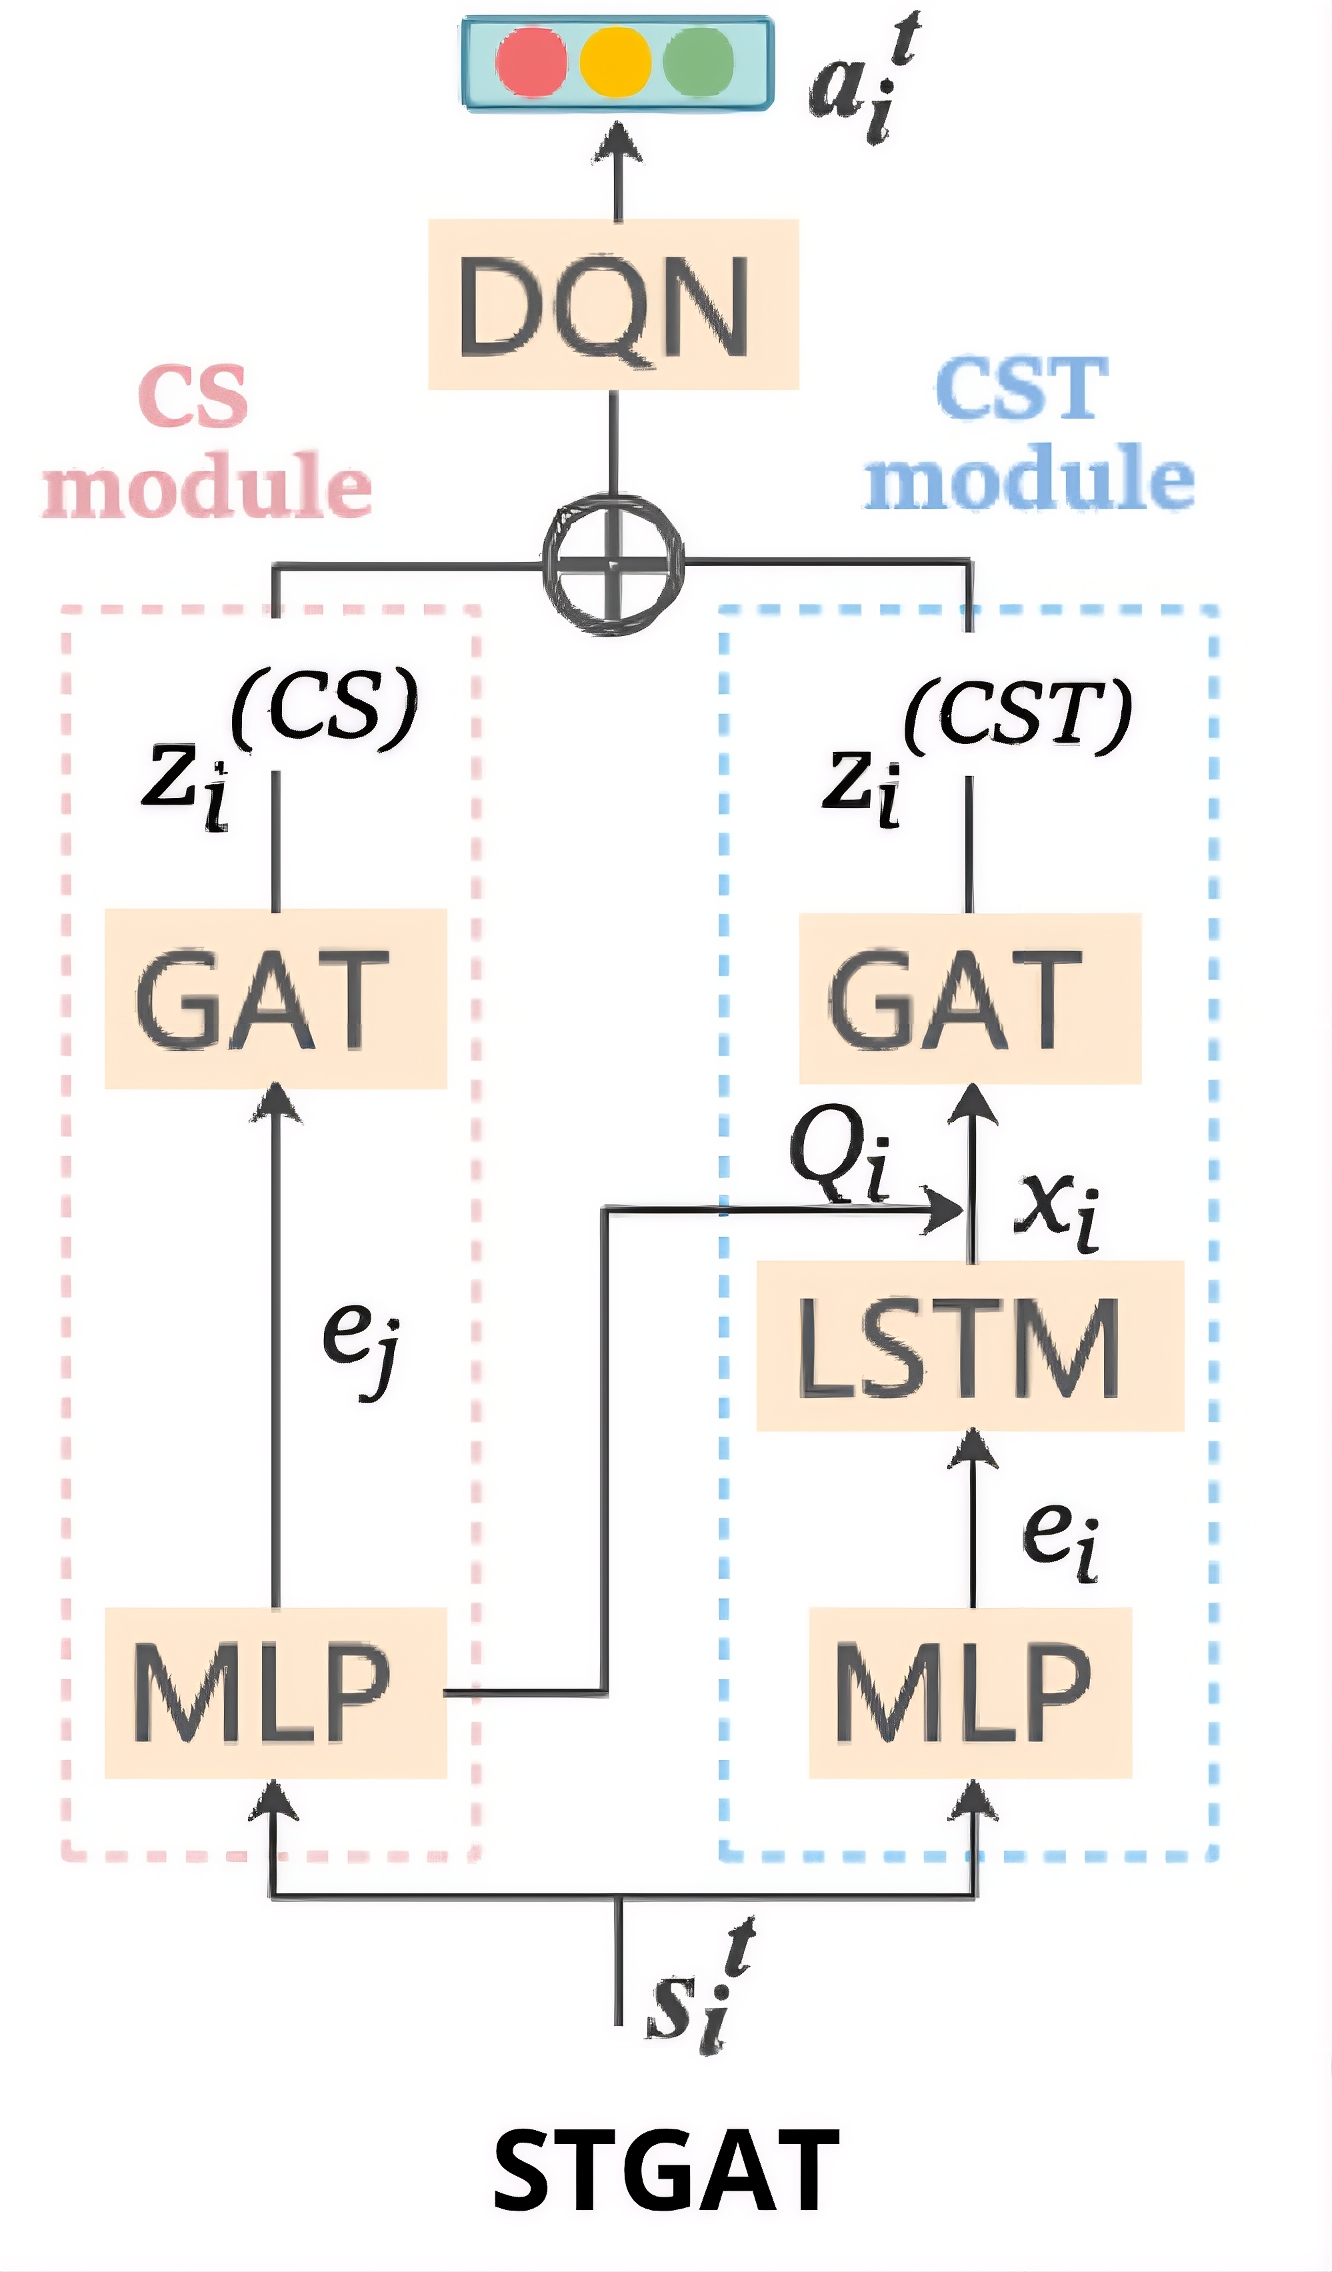
\includegraphics[width=0.55\textwidth]{architettura_stgat.png}
  \caption{Schema a blocchi dell'architettura STGAT: dallo stato dell'intersezione
    $s_i^t$, attraverso l'encoder duale (MLP) e i moduli CS e CST (GAT e LSTM a
    pesi condivisi), fino all'azione $a_i^t$ scelta dal Double DQN (il
    blocco "DQN" della figura, adattata dal riferimento originale, ne
    indica la testa dei Q-value). Adattato da
    \citet{wang2022metastgat}.}
  \label{fig:stgat-architettura}
\end{figure}

\subsection{State Encoder duale}
\label{subsec:state-encoder}

Lo stato $s_i^t \in \mathbb{R}^{d_0}$ ($d_0=32$ o $20$, §\ref{sec:formalizzazione}) di un incrocio $i$ al tempo $t$
attraversa due Multilayer Perceptron (MLP) a due strati con la stessa architettura ma pesi e
inizializzazioni indipendenti:
\begin{align}
  e_i^t & = \mathrm{MLP_t}(s_i^t) = \sigma\big(W_{21}\,\sigma(W_{11} s_i^t + b_{11}) + b_{21}\big) \in \mathbb{R}^{d_1} \\
  e_j^t & = \mathrm{MLP_s}(s_i^t) = \sigma\big(W_{22}\,\sigma(W_{12} s_i^t + b_{12}) + b_{22}\big) \in \mathbb{R}^{d_1}
\end{align}
dove $d_1$ viene fissato a $64$, $W_{11},W_{12}\in\mathbb{R}^{d_1\times d_0}$ e $W_{21},W_{22}\in\mathbb{R}^{d_1\times d_1}$ sono i pesi,
$b_{11}, b_{21}, b_{12}, b_{22}\in\mathbb{R}^{d_1}$ i bias e
$\sigma$ la funzione di attivazione ReLU. Il pedice $j$ in $e_j^t$ è
un'etichetta del ramo spaziale, coerente con la notazione delle figure di
questa sezione, non l'indice di un nodo vicino: anche $e_j^t$ è calcolato
a partire dallo stato $s_i^t$ del nodo stesso.

Il vettore $e_i^t = \mathrm{MLP_t}(s_i^t)$ verrà usato come input nella LSTM e veicolerà le caratteristiche temporali dello stato,
mentre $e_j^t = \mathrm{MLP_s}(s_i^t)$ verrà usato come input nelle GAT, catturando le caratteristiche spaziali dello stesso.


\subsection{Modulo spazio-temporale corrente (CST)}
\label{subsec:cst-module}

Nel momento di una decisione, un conteggio istantaneo dei veicoli, da solo, non distingue una coda che si
sta formando da una che si sta esaurendo. Due situazioni che possono
richiedere una fase diversa appaiono dunque identiche a un modello privo
di memoria. Il primo dei due moduli di STGAT viene introdotto per questo motivo:
combina l'informazione temporale accumulata da un'intersezione con
l'informazione spaziale corrente di sé stessa e dei suoi vicini, così che la scelta dell'azione
possa tenere conto di come il traffico più ravvicinato si sta
evolvendo, non solo di come si presenta localmente nell'istante attuale.
Wang et al. (2022) motivano questo modulo osservando che altri lavori
sulle Spatio-Temporal Graph Neural Networks (STGNN) propongono strutture
simili, ma vi combinano le informazioni spaziali e temporali in un unico
embedding oppure le usano separatamente; con il modulo CST cercano invece
di intrecciare le due informazioni in modo più elaborato.

Il ramo temporale dell'encoder $e_i^t$ (§\ref{subsec:state-encoder})
attraversa anzitutto una cella LSTM con pesi condivisi da ogni nodo della rete:
\begin{equation}
  \begin{bmatrix} f_i^t \\ \iota_i^t \\ o_i^t \\ g_i^t \end{bmatrix} =
  \begin{bmatrix} \sigma \\ \sigma \\ \sigma \\ \tanh \end{bmatrix}
  \left(
  W_{\{f,\iota,o,g\}}^{\top} [\,e_i^t \,\|\, h_i^{t-1}\,] + b_{\{f,\iota,o,g\}}
  \right),
  \label{eq:stgat-lstm-gates}
\end{equation}
\[ c_i^t = f_i^t \odot c_i^{t-1} + \iota_i^t \odot g_i^t, \]
\[ x_i^t = h_i^t = o_i^t \odot \tanh(c_i^t); \]
in notazione compatta:
\begin{equation}
  \big(h_i^t,\, c_i^t\big) = \mathrm{LSTM}\big(e_i^t \,;\, h_i^{t-1},\, c_i^{t-1}\big).
  \label{eq:stgat-lstm-compact}
\end{equation}
Il vettore $x_i^t := h_i^t$ prodotto da questa cella rappresenta concettualmente un riassunto temporale dei flussi di traffico locali.

Lo stesso vettore, nel meccanismo di attenzione che segue, diventa l'informazione che i vicini dell'incrocio $i$ "leggono"
per decidere quanto pesare il contributo di $i$ nel proprio contesto locale. Questa trasmissione di informazione avviene
tramite l'applicazione di una Graph Attention Network (GAT) con una rappresentazione differente rispetto a
quella della GAT standard di \citet{velickovic2018gat} riportata nel Capitolo~\ref{cap:background}.
In tale GAT infatti ciascun nodo viene comparato con gli altri nodi secondo una stessa proiezione dell'embedding.
Nella struttura proposta invece, prendendo ispirazione da approcci di machine translation \citep{vaswani2017attention}, i nodi si influenzano vicendevolmente secondo valori distinti: Query, Key e Value.
In particolare si scelgono come Query $Q=e_j^t$ (la codifica spaziale corrente del nodo ricevente) e come Key e Value $K=V=x_i^t$ (la memoria temporale di ciascun vicino).
L'idea alla base di questa scelta è il tentativo di arricchire le caratteristiche temporali correnti di ciascun nodo con la memoria temporale dei flussi dello stesso e dei nodi vicini.
Si precisa che nel caso di $H>1$ teste di attenzione, come in questo lavoro, i valori $Q,K,V$ non sono proiettati da matrici distinte per ciascuna testa, bensì
il vettore a $d_1$ componenti viene partizionato in $H$ segmenti contigui di dimensione $d_h = d_1/H$, e la testa $h$ opera sul solo blocco $Q_h(i) := Q(i)[h d_h : (h{+}1)d_h]$ (analogamente per $K_h(u)$, $V_h(u)$).
Le teste restano quindi distinte perché leggono porzioni diverse dello stesso embedding, non perché dispongano di proiezioni apprese proprie.

Formalmente, nel caso in esame, per ciascun nodo $i$ con vicinato $\mathcal{N}(i)$ (con $i\in \mathcal{N}(i)$) e $h$ una delle $H=4$ teste di dimensione $d_h = d_1/H = 16$, questo modulo di GAT viene descritto come segue:
\begin{equation}
  \varphi_h(i,u) = \frac{Q_h(i) \cdot K_h(u)}{\sqrt{d_h}} ,
  \label{eq:stgat-attn}
\end{equation}
\[ \alpha_h(i,u) = \frac{\exp(\varphi_h(i,u))}{\sum_{u' \in \mathcal{N}(i)} \exp(\varphi_h(i,u'))}, \]
\begin{equation}
  z_h(i) = \sum_{u \in \mathcal{N}(i)} \alpha_h(i,u)\, V_h(u) .
  \label{eq:stgat-z}
\end{equation}

L'output finale di questo modulo spazio-temporale corrente sarà
\begin{equation}
  z_{\mathrm{CST}}(i) = [z_1(i) \| \dots \| z_H(i)] \in \mathbb{R}^{d_1}.
  \label{eq:stgat-cst-output}
\end{equation}
Auspicabilmente, in questo stato è racchiusa una sintesi delle dinamiche spaziali e temporali del traffico locale e degli incroci adiacenti.


\subsection{Modulo spaziale corrente (CS)}
\label{subsec:cs-module}

Il modulo spazio-temporale, filtrato dalla memoria della cella ricorrente,
può attenuare segnali che sono invece rilevanti nell'istante
presente; ad esempio un picco di traffico simultaneo su un intero asse
necessita di coordinamento spaziale puro, a prescindere dalla durata del picco stesso.
Questo secondo modulo, strutturalmente simile al primo,
elabora perciò la sola informazione spaziale corrente $e_j^t$, senza alcuna
componente di memoria.
Il vettore $e_j^t$ attraversa una GAT che opera secondo le stesse dinamiche descritte
nel paragrafo precedente, ma con l'assegnazione $Q=K=V=e_j^t$.
L'output finale del modulo spaziale corrente sarà
\begin{equation}
  z_{\mathrm{CS}}(i) = [z_1(i) \| \dots \| z_H(i)] \in \mathbb{R}^{d_1} ,
  \label{eq:stgat-cs-output}
\end{equation}
Tale rappresentazione del traffico permetterà al modello di focalizzarsi sulla coordinazione dei nodi rispetto alla sola fotografia presente della rete.

\subsection{Testa Q-value}
\label{subsec:q-head}

Le due uscite, $z_{\mathrm{CST}}(i)$ e $z_{\mathrm{CS}}(i)$, catturano
quindi aspetti complementari, l'uno informato dalla memoria temporale dei
vicini, l'altro dalla sola situazione presente. Tali vettori vengono infine concatenati e attraversano un singolo layer lineare per
produrre la stima del valore di ciascuna delle 8 azioni eseguibili all'incrocio $i$ e all'istante $t$:
\begin{equation}
  q(s_i^t, \cdot\,) = W_q\,[\,z_{\mathrm{CST}}(i) \,\|\, z_{\mathrm{CS}}(i)\,] + b_q \in \mathbb{R}^{8}
\end{equation}
dove $W_q \in \mathbb{R}^{8 \times 2 d_1}$ e $b_q \in \mathbb{R}^{8}$.

\subsection{Meta-knowledge learner}

I due moduli appena descritti, alla base della struttura STGAT, condividono gli stessi pesi
per ogni intersezione della rete, indipendentemente dal ruolo che occupa.
Ad esempio un incrocio periferico, uno pienamente interno alla rete stradale, o uno
attraversato da un'arteria a densità di traffico elevata
(§\ref{subsec:dataset}) applicano esattamente la stessa regola di coordinamento.
MetaSTGAT introduce un meccanismo di meta-apprendimento che condiziona
tale regola su un embedding di caratteristiche locali dell'incrocio,
cosicché i layer di GAT e di LSTM possano specializzarsi
rispetto alle condizioni osservate da ciascun nodo invece di applicare la stessa
funzione ovunque. L'idea alla base di questo meccanismo, condivisa da
entrambi i componenti "meta" che seguono, è illustrata in
Figura~\ref{fig:meta-learning-overview}: le meta-feature spaziali e
temporali, elaborate da un meta-learner dedicato, generano i pesi dei layer
di LSTM e GAT al posto di parametri fissi condivisi da ogni nodo.

\begin{figure}[htbp]
  \centering
  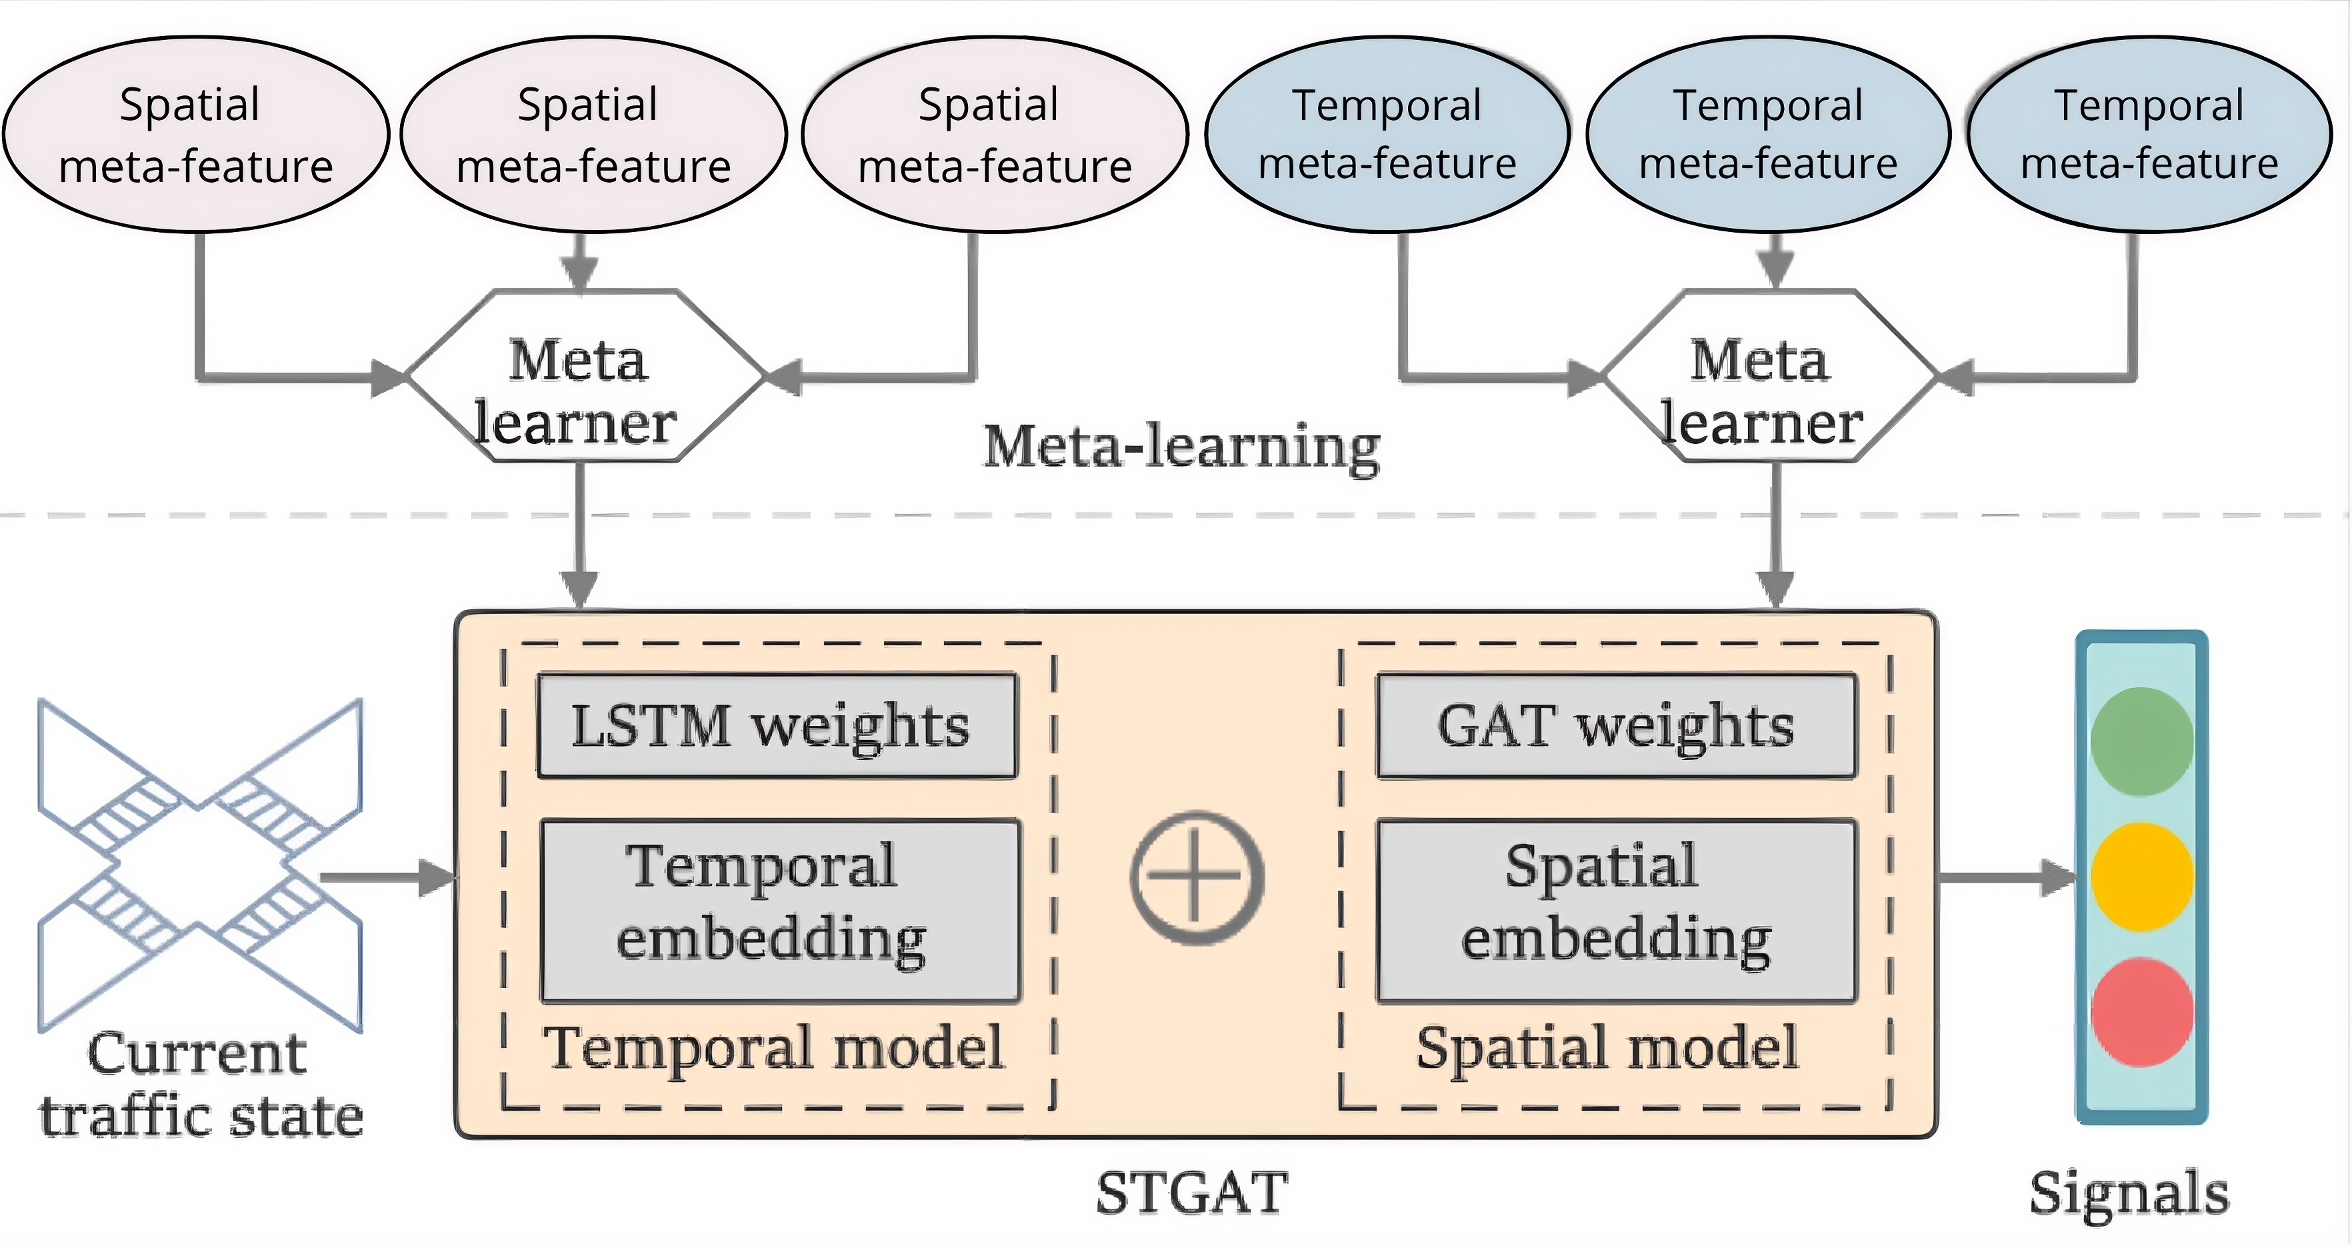
\includegraphics[width=0.75\textwidth]{meta_learning_overview.png}
  \caption{Principio del meta-apprendimento applicato da MetaSTGAT: le
    meta-feature spaziali e temporali condizionano, tramite un meta-learner
    dedicato, i pesi dei layer LSTM e GAT usati per elaborare lo stato corrente
    del traffico. Adattato da \citet{wang2022metastgat}.}
  \label{fig:meta-learning-overview}
\end{figure}

In particolare, due MLP a due strati, uno per l'aspetto spaziale e uno per quello temporale del
problema, apprendono un embedding di caratteristiche locali dell'intersezione (Spatial Meta-Knowledge, SMK; Temporal Meta-Knowledge, TMK)
a partire dalle meta-feature che descrivono il nodo ($x^{\mathrm{smk}}_i$ e $x^{\mathrm{tmk}}_i$):
\begin{align}
  \mathrm{SMK}(i) & = \mathrm{MLP}_{\mathrm{smk}}\big(x^{\mathrm{smk}}_i\big) \in \mathbb{R}^{64} \\
  \mathrm{TMK}(i) & = \mathrm{MLP}_{\mathrm{tmk}}\big(x^{\mathrm{tmk}}_i\big) \in \mathbb{R}^{64}
\end{align}
Come già accennato, tali valori verranno poi usati per generare i pesi di Meta-GAT e Meta-LSTM,
tramite dei MLP addizionali specializzati per ciascuno dei moduli, secondo quanto riporteremo in
(§\ref{subsec:meta-gat}) e (§\ref{subsec:meta-lstm}).
Il passaggio dalle meta-feature grezze ai due embedding $\mathrm{SMK}(i)$ e
$\mathrm{TMK}(i)$ è riassunto graficamente in Figura~\ref{fig:meta-knowledge-learner}.

\begin{figure}[htbp]
  \centering
  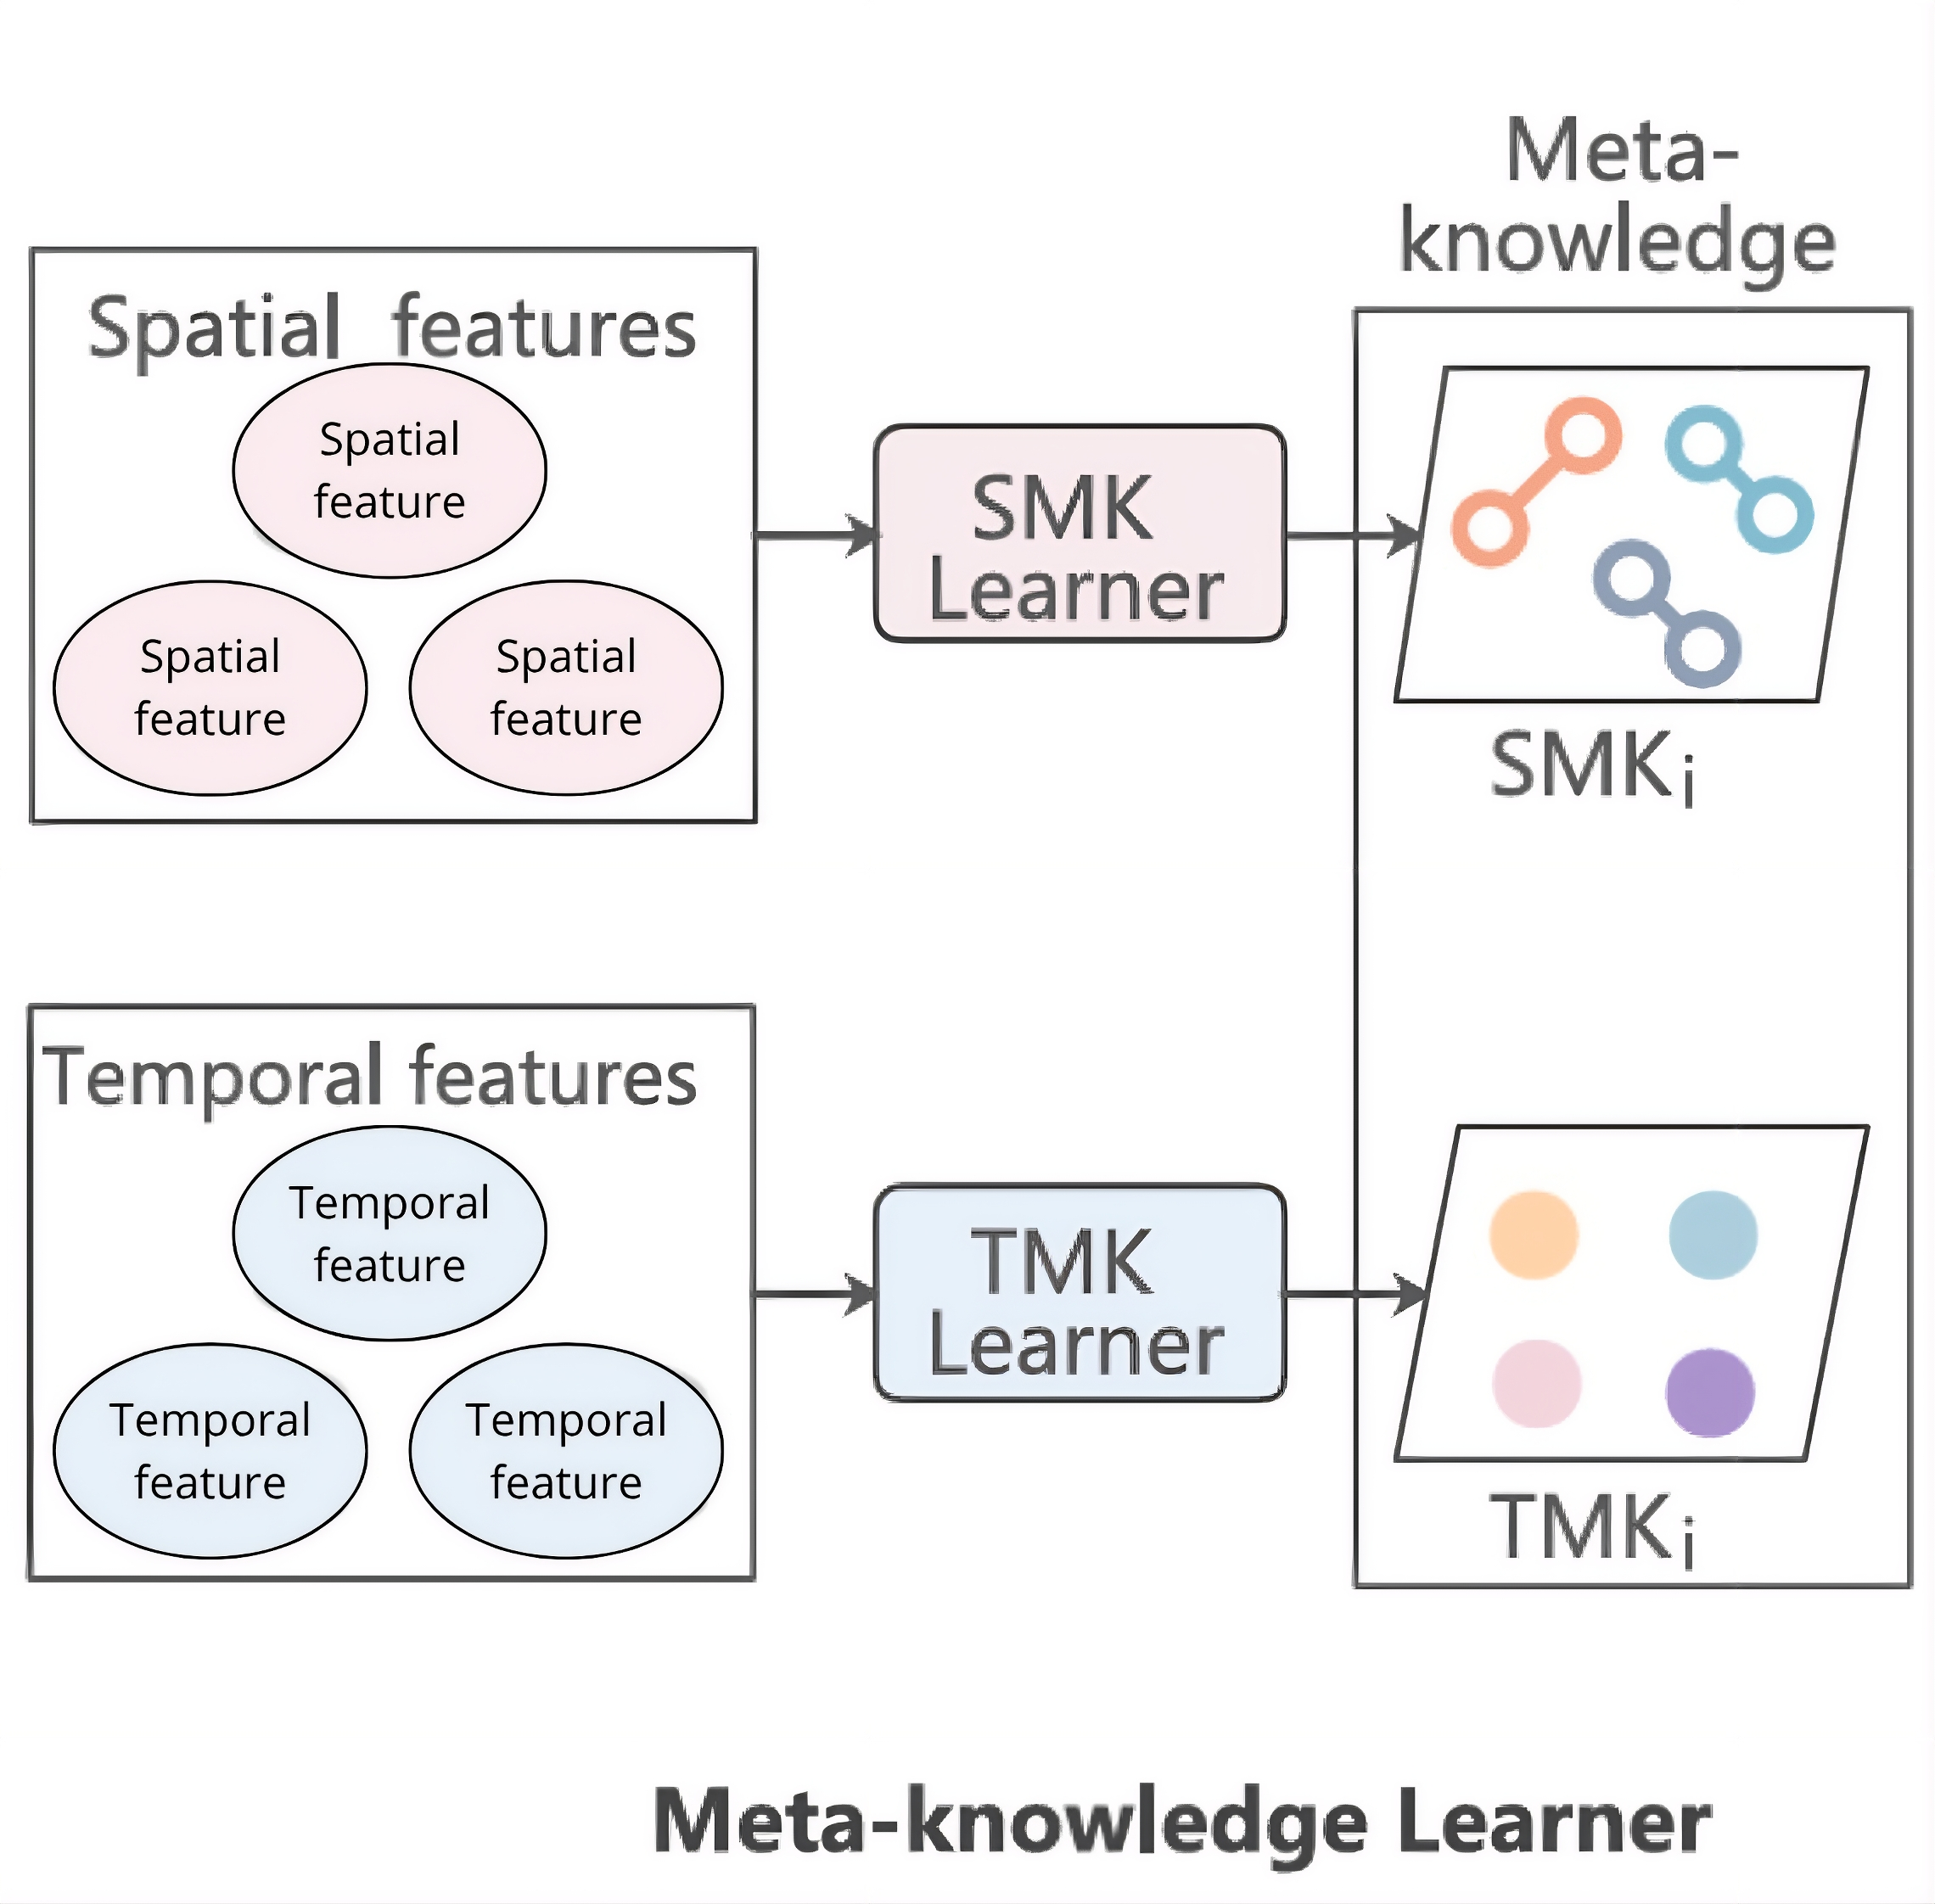
\includegraphics[width=0.7\textwidth]{meta_knowledge_learner.png}
  \caption{Il Meta-knowledge Learner: le meta-feature spaziali e temporali
    grezze vengono elaborate rispettivamente dallo SMK-Learner e dal TMK-Learner,
    producendo gli embedding $\mathrm{SMK}(i)$ e $\mathrm{TMK}(i)$ usati da
    Meta-GAT e Meta-LSTM. Adattato da \citet{wang2022metastgat}.}
  \label{fig:meta-knowledge-learner}
\end{figure}

Le meta-feature $x^{\mathrm{smk}}_i$ e $x^{\mathrm{tmk}}_i$ riprendono
l'insieme di informazioni del riferimento originale, adattato in questo
lavoro; sono pensate per fornire al modello informazioni aggiuntive che ne
consentano una migliore specializzazione rispetto al contesto specifico
di ciascun incrocio.

Il vettore spaziale $x^{\mathrm{smk}}_i \in \mathbb{R}^{26}$ concatena cinque gruppi di feature, ciascuno variabile da nodo a nodo:
\begin{itemize}
  \item pressione per corsia [12]: per ciascuna corsia, la differenza tra i veicoli in ingresso sulla corsia e la media dei veicoli sulle corsie in uscita raggiungibili da essa, divisa per 30;
  \item numero di incroci adiacenti [1]: frazione tra il numero di vicini del nodo e il massimo previsto dalla topologia a griglia (4), distingue quindi un incrocio d'angolo, di bordo o interno;
  \item differenza tra la pressione media propria e quella di ciascun incrocio adiacente [4]: per ciascuno dei vicini, la pressione media delle 12 corsie del nodo meno quella del vicino, con zero-padding negli slot oltre il numero di vicini effettivamente presenti;
  \item asimmetria di pressione tra le corsie N/S e le corsie E/O dello stesso nodo [1]: media della pressione sulle 6 corsie N/S meno la media sulle 6 corsie E/O;
  \item pressione per fase [8]: la stessa quantità dell'Equazione~\ref{eq:maxpressure-phase}, usata da Max-Pressure (§\ref{subsec:tsc-generations}) per decidere la fase da selezionare, una componente per ciascuna delle 8 fasi.
\end{itemize}
Il costo di raccolta di queste feature si limita a sensori con la stessa capacità visiva già richiesta per lo stato principale e per il reward, sia sulle corsie in ingresso sia su quelle in uscita: le feature di pressione si misurano semplicemente contando i veicoli su queste corsie, mentre il numero di incroci adiacenti è un dato topologico costante per ciascun incrocio.

Il vettore di meta-feature temporali $x^{\mathrm{tmk}}_i \in \mathbb{R}^{25}$
concatena invece tre diversi tipi di informazione, tutte variabili nel tempo all'interno dello stesso nodo:
\begin{itemize}
  \item variazione della coda per corsia rispetto a 3 passi precedenti [12]: per ciascuna corsia, differenza tra il numero di veicoli in coda all'istante corrente e quello di 3 step prima;
  \item durata di permanenza della fase corrente [1]: numero di step consecutivi in cui la fase è rimasta attiva, saturato e normalizzato in $[0,1]$ rispetto a un tetto di 2 step, oltre il quale la maschera anti-starvation di questo lavoro (§\ref{sec:formalizzazione}) impone comunque un cambio di fase;
  \item deviazione standard della coda per corsia sulla finestra recente [12]: calcolata sugli ultimi 5 step disponibili.
\end{itemize}
Anche queste feature vengono calcolate a partire da informazioni fornite dal simulatore e non richiedono strumenti aggiuntivi.

Si noti come nessuna di queste feature entri anche nello stato principale: la scelta
è legata alla volontà di non appesantire lo stato del sistema, sfruttando le stesse
per agire direttamente sui pesi che regolano la trasmissione dell'informazione.

\subsection{Meta-GAT}
\label{subsec:meta-gat}

La versione meta delle GAT usate in STGAT riprende la struttura architetturale delle stesse,
ma implementa delle modifiche mirate a consentire ai layer di apprendere regole di aggregazione spaziale
dipendenti dalle caratteristiche del singolo nodo.
I valori assegnati a $Q, K, V$ rimangono invariati, sia per il modulo spaziale
($Q=K=V=e_j^t$) sia per il modulo spazio-temporale ($Q=e_j^t$, $K=V=x_i^t$).
L'unica differenza riguarda l'inserimento, nel punteggio di compatibilità dell'Equazione~\ref{eq:stgat-attn},
di una trasformazione lineare per nodo che in STGAT non esiste: il modulo CS
riceve il proprio meta-embedding da $\mathrm{SMK}(i)$, il modulo CST da
$\mathrm{TMK}(i)$, in modo che la regola di attenzione spaziale e quella
spazio-temporale si adattino a caratteristiche locali diverse.
In particolare, per ciascun nodo $i$ e ciascuna testa $h$, una rete
$\mathrm{MLP}_{\mathrm{GAT,smk},h}$ condivisa da tutti i nodi genera, dal
solo embedding meta del nodo ricevente, i pesi del modulo spaziale:
\begin{equation}
  W_{j,h}^{(i)}, \, b_{j,h}^{(i)} = \mathrm{MLP}_{\mathrm{GAT,smk},h}\big( \mathrm{SMK}(i) \big) \in \mathbb{R}^{d_h \times d_h}, \mathbb{R}
  \label{eq:metagat-hyper-smk}
\end{equation}
e analogamente, tramite $\mathrm{MLP}_{\mathrm{GAT,tmk},h}$, per il modulo spazio-temporale:
\begin{equation}
  W_{k,h}^{(i)}, \, b_{k,h}^{(i)} = \mathrm{MLP}_{\mathrm{GAT,tmk},h}\big( \mathrm{TMK}(i) \big) \in \mathbb{R}^{d_h \times d_h}, \mathbb{R}
  \label{eq:metagat-hyper-tmk}
\end{equation}
dove le iper-reti $\mathrm{MLP}$ sono composte da due layer, condivise da
tutti i nodi della rete: solo il loro output dipende da $i$, tramite
l'input $\mathrm{SMK}(i)$ o $\mathrm{TMK}(i)$.
E dunque, per ogni nodo $u \in \mathcal{N}(i)$:
\begin{equation}
  \varphi_h(i,u) = \frac{\big(W_h^{(i)} Q_h(i)\big) \cdot K_h(u) + b_h^{(i)}}{\sqrt{d_h}} ,
  \label{eq:metagat-attn}
\end{equation}
\[ \alpha_h(i,u) = \frac{\exp(\varphi_h(i,u))}{\sum_{u' \in \mathcal{N}(i)} \exp(\varphi_h(i,u'))} ,\]
\[ z_h(i) = \sum_{u \in \mathcal{N}(i)} \alpha_h(i,u)\, V_h(u) ,\]
\[ z(i) = \big[z_1(i) \,\|\, \dots \,\|\, z_H(i)\big] \in \mathbb{R}^{d_1} ,\]
con $W_h^{(i)}$ e $b_h^{(i)}$ relativo al proprio modulo di riferimento.
La Figura~\ref{fig:meta-gat-diagramma} mette a confronto i due moduli appena
descritti, evidenziando come SMK e TMK alimentino iper-reti distinte per
generare i pesi $(W,b)$ specifici di ciascuno.

\begin{figure}[htbp]
  \centering
  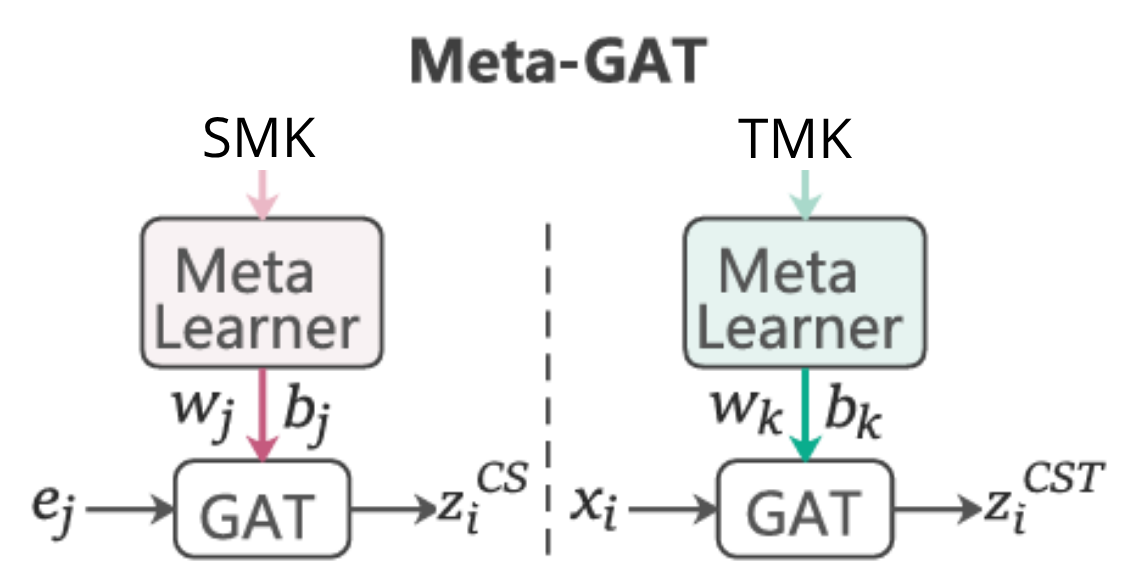
\includegraphics[width=0.8\textwidth]{meta_gat_diagramma.png}
  \caption{Meta-GAT: il modulo CS (sinistra) genera i pesi $(W_j, b_j)$ della
    propria GAT a partire da $\mathrm{SMK}$, il modulo CST (destra) genera
    $(W_k, b_k)$ a partire da $\mathrm{TMK}$; entrambi producono l'output $z_i$
    del rispettivo modulo. Adattato da \citet{wang2022metastgat}.}
  \label{fig:meta-gat-diagramma}
\end{figure}

\subsection{Meta-LSTM}
\label{subsec:meta-lstm}

Meta-LSTM applica alla cella ricorrente di STGAT
la stessa generalizzazione che Meta-GAT applica al \emph{graph attention}:
i pesi $W_{(f, \iota, o, g)}$ e i bias $b_{(f, \iota, o, g)}$ condivisi in STGAT da ogni nodo della rete,
sono qui sostituiti da pesi e bias generati individualmente per ogni nodo.

Un MLP a due layer per ciascun gate genera, dal solo $\mathrm{TMK}(i)$, i pesi \\
$W_{(f, \iota, o, g)}^{(i)} \in \mathbb{R}^{2d_1 \times d_1}$ e i bias $b_{(f, \iota, o, g)}^{(i)} \in \mathbb{R}^{d_1}$,
modificando l'Equazione~\ref{eq:stgat-lstm-gates} come segue:
\begin{equation}
  \begin{bmatrix} f_i^t \\ \iota_i^t \\ o_i^t \\ g_i^t \end{bmatrix} =
  \begin{bmatrix} \sigma \\ \sigma \\ \sigma \\ \tanh \end{bmatrix}
  \left(
  \Big(W_{\{f,\iota,o,g\}}^{(i)}\Big)^{\!\top} [\,e_i^t \,\|\, h_i^{t-1}\,] + b_{\{f,\iota,o,g\}}^{(i)}
  \right)
  \label{eq:metalstm-gates}
\end{equation}
\begin{equation}
  c_i^t = f_i^t \odot c_i^{t-1} + \iota_i^t \odot g_i^t
\end{equation}
\begin{equation}
  x_i^t = h_i^t = o_i^t \odot \tanh(c_i^t)
\end{equation}
In notazione compatta, esplicitando la sola dipendenza aggiuntiva dai pesi
generati dal meta-learner:
\begin{equation}
  \big(h_i^t,\, c_i^t\big) = \mathrm{LSTM}\Big(e_i^t \,;\, h_i^{t-1},\, c_i^{t-1} \;\Big|\; W_{\{f,\iota,o,g\}}^{(i)},\, b_{\{f,\iota,o,g\}}^{(i)}\Big), \qquad x_i^t := h_i^t.
  \label{eq:metalstm-compact}
\end{equation}
L'output $x_i^t$ alimenta il modulo CST di Meta-GAT come $K$ e $V$ (§\ref{subsec:meta-gat}),
analogamente a quanto visto con STGAT.
L'architettura appena descritta è riassunta graficamente in Figura~\ref{fig:meta-lstm-diagramma},
dove $W_{\Phi},b_{\Phi}$ indicano genericamente i pesi e i bias generati dal meta-learner.

\begin{figure}[htbp]
  \centering
  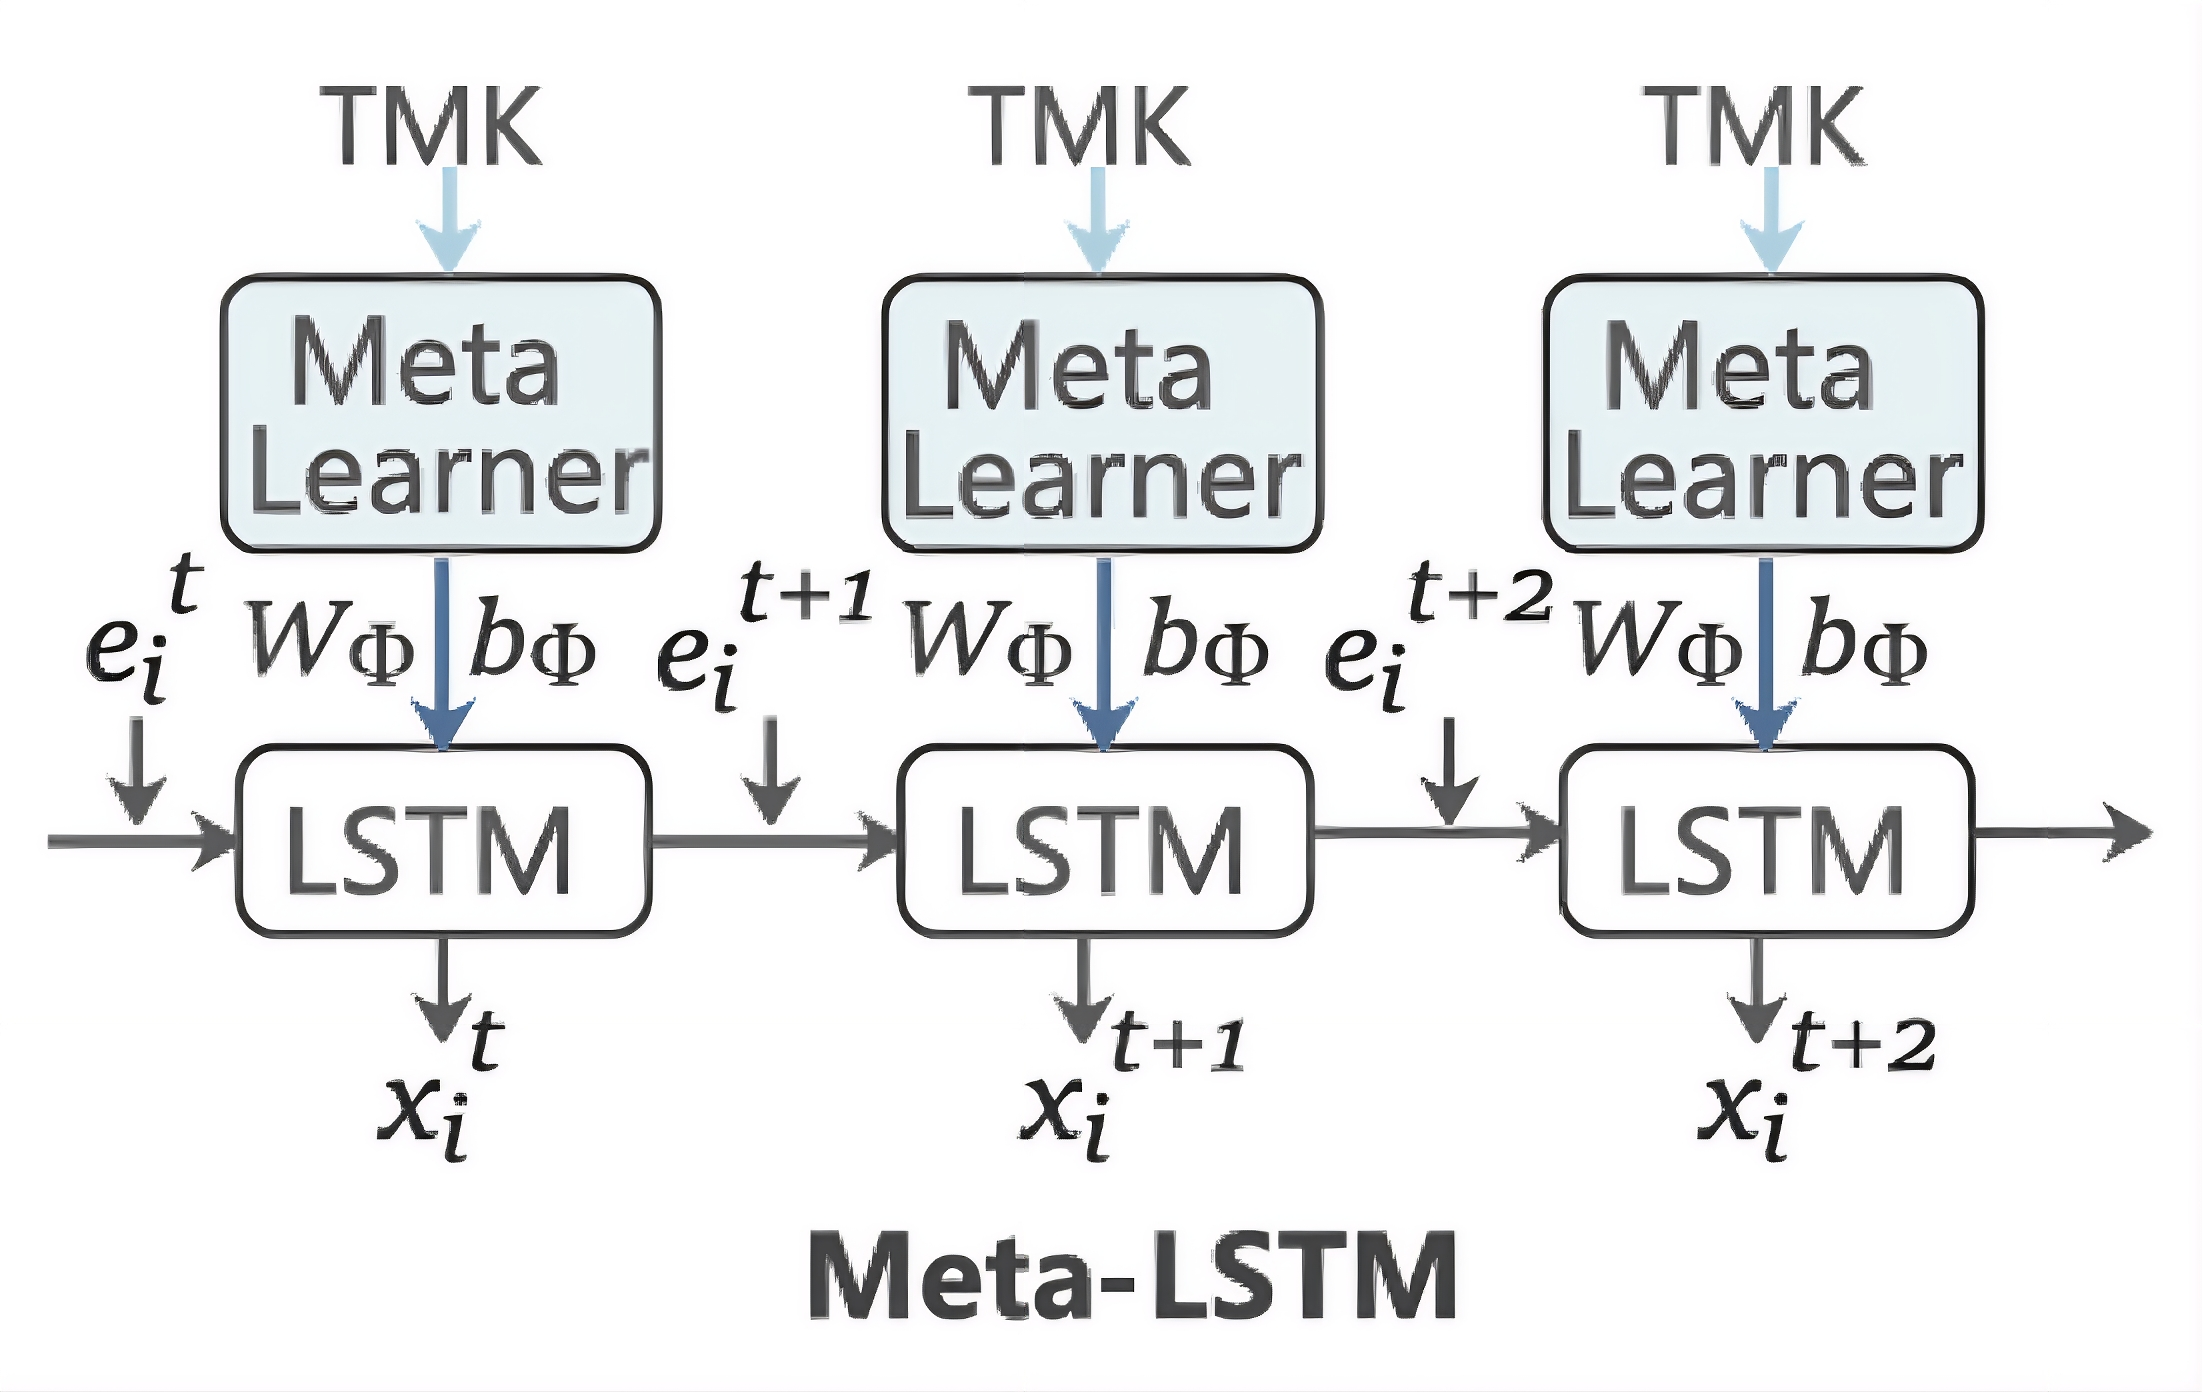
\includegraphics[width=0.85\textwidth]{meta_lstm_diagramma.png}
  \caption{Meta-LSTM "srotolata" nel tempo: a ogni istante $t$ il meta-learner
    genera, da $\mathrm{TMK}(i)$, i pesi $W_\Phi$ e $b_\Phi$ della cella LSTM
    che produce $x_i^t$ dall'input $e_i^t$ e dallo stato nascosto precedente $h_i^{t-1}, c_i^{t-1}$.
    Adattato da \citet{wang2022metastgat}.}
  \label{fig:meta-lstm-diagramma}
\end{figure}

Messi insieme, i moduli descritti in questa sezione compongono
l'architettura di Figura~\ref{fig:architettura-metastgat}, che ne riassume
il flusso complessivo dallo stato $s_i^t$ all'azione scelta.

\begin{figure}[htbp]
  \centering
  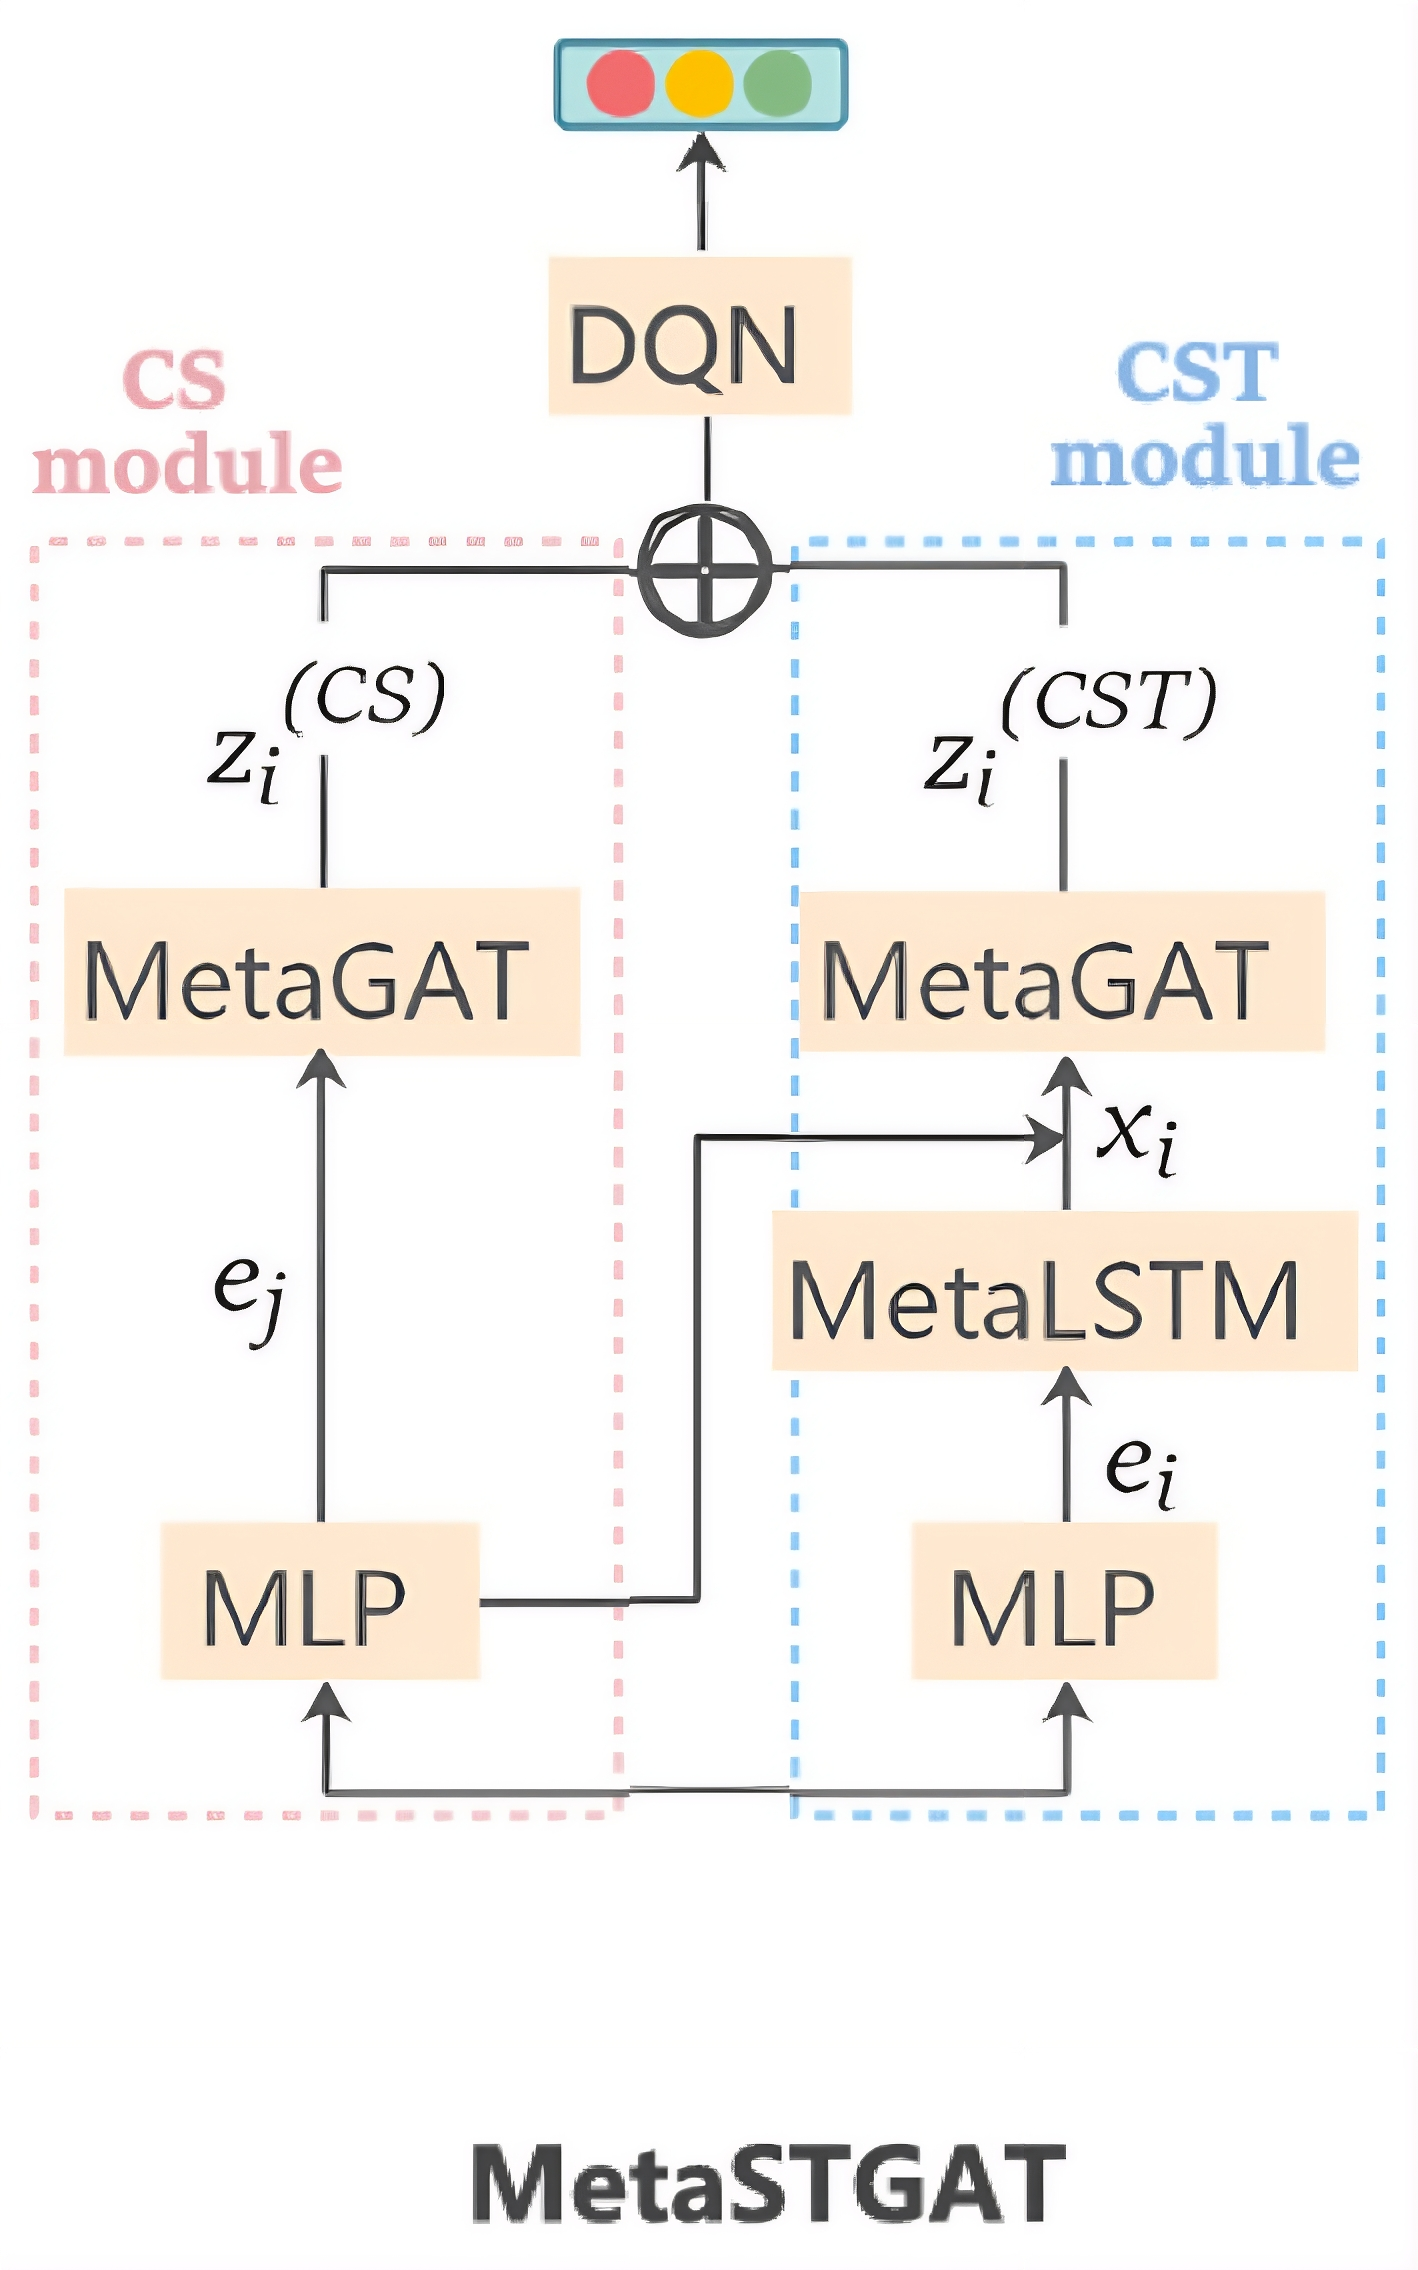
\includegraphics[width=0.5\textwidth]{architettura_metastgat.png}
  \caption{Schema a blocchi completo di MetaSTGAT: rispetto a STGAT
    (Figura~\ref{fig:stgat-architettura}), GAT e LSTM sono sostituiti dalle
    rispettive versioni meta-condizionate, con i pesi generati dagli embedding
    $\mathrm{SMK}(i)$ e $\mathrm{TMK}(i)$ del Meta-knowledge Learner. Adattato
    da \citet{wang2022metastgat}.}
  \label{fig:architettura-metastgat}
\end{figure}

\subsection{Meccanismi spaziali alternativi}
\label{sec:spatial-alt}

Il modulo Meta-GAT decide quanto ciascun vicino debba contribuire
all'aggiornamento di un'intersezione tramite un punteggio di compatibilità
appreso, specifico per ogni nodo (§\ref{subsec:meta-gat}).
Questa formulazione rappresenta tuttavia solo una delle possibili declinazioni del paradigma di \emph{message passing} su grafo.
Con l'obiettivo di esplorare soluzioni alternative, in questa sezione
vengono introdotte ed estese in chiave meta-learning due diverse
architetture di aggregazione spaziale: Meta-GCN e Meta-SONAR, presentate
come sostituzione del solo blocco GAT di Figura~\ref{fig:architettura-metastgat}, a parità di tutto il resto.

Ogni altro componente dell'architettura (encoder di stato, meta-learner
spaziale e temporale, Meta-LSTM, testa Q-value) e la procedura di training (§\ref{sec:training}) rimangono invariati:
a parità di tutto il resto, le differenze di prestazione misurate nel
Capitolo~\ref{cap:confronto} si possono quindi ricondurre principalmente
al solo meccanismo di aggregazione spaziale, entro la variabilità tra
seed.

La prima architettura, una \emph{graph convolution network} (GCN), rimuove il punteggio di compatibilità della GAT e lo sostituisce
con un peso fisso determinato solo dalla topologia.
La seconda, una propagazione ondulatoria a lungo raggio chiamata SONAR \citep{trenta2025sonar},
sostituisce l'aggregazione a un passo con l'evoluzione discretizzata di un sistema dinamico su più iterazioni interne.

In entrambi i casi il principio "meta" resta identico a Meta-GAT:
i pesi dell'aggregazione sono generati da un embedding SMK/TMK per ciascun nodo, non appresi come parametro fisso condiviso.

\subsubsection{Meta-GCN}
\label{subsec:meta-gcn}

La GCN \citep{kipf2017gcn}, introdotta nel Capitolo~\ref{cap:background}
(Equazione~\ref{eq:gcn-aggregate}), pesa il contributo di ogni vicino con la
normalizzazione simmetrica del grado: una quantità che dipende solo dalla
topologia della rete, mai dal contenuto dello stato dei nodi coinvolti. È
dunque il termine di paragone più diretto per isolare cosa aggiunge il
punteggio di compatibilità di Meta-GAT: sostituendolo con questa regola
fissa, e lasciando invariato tutto il resto dell'architettura, ogni
differenza di prestazioni misurata nel Capitolo~\ref{cap:confronto} è
imputabile a quel solo meccanismo.

Per un nodo $i$, con $\mathcal{N}(i)$ il suo vicinato (incluso il self-loop
permanente di questo lavoro, §\ref{sec:formalizzazione}) e $\hat d_i =
  |\mathcal{N}(i)|$ il grado corrispondente, il principio meta genera $W$ e
$b$ per ciascun nodo ricevente $i$, a partire dal suo embedding meta $m_i$
(pari a $\mathrm{SMK}(i)$ per il modulo CS e a $\mathrm{TMK}(i)$ per il
modulo CST), tramite un'iper-rete a due strati condivisa da tutti i nodi,
in modo analogo a quanto visto in Meta-GAT:
\[
  W^{(i)}, \, b^{(i)} = \mathrm{MLP}_{\mathrm{GCN},m}\big(m_i\big) \in \mathbb{R}^{d_1 \times d_1}, \, \mathbb{R}
\]
Poi, per ogni nodo $i$, la regola di aggregazione, che nella versione
originale non-meta della GCN userebbe una matrice $W$ condivisa da ogni
nodo della rete (Equazione~\ref{eq:gcn-aggregate}), diventa:
\begin{equation}
  z(i) = \sigma\Bigg(\bigg(\sum_{u \in \mathcal{N}(i)} \frac{1}{\sqrt{\hat d_i \hat d_u}}\, W^{(i)}V(u)\bigg) + b^{(i)}\Bigg)
  \label{eq:metagcn}
\end{equation}
dove $\sigma$ è la funzione di attivazione ReLU e $V(u)$ il valore del
nodo $u$ ($h_u$ nell'Equazione~\ref{eq:gcn-aggregate} del
Capitolo~\ref{cap:background}). Come per Meta-GAT, il modulo CST assegna
$V=x_i^t$ (l'uscita della Meta-LSTM, §\ref{subsec:meta-lstm}) e
$m_i=\mathrm{TMK}(i)$; il modulo CS assegna $V=e_j^t$ e
$m_i=\mathrm{SMK}(i)$.

\subsubsection{Meta-SONAR}
\label{subsec:meta-sonar}

Sia Meta-GAT sia Meta-GCN propagano informazione a un solo passo di
distanza per ogni applicazione del layer: raggiungere un vicino a $k$
archi di distanza richiede $k$ applicazioni. SONAR \citep{trenta2025sonar},
introdotto nel Capitolo~\ref{cap:background} (§\ref{sec:background-gnn}),
evita questo costo modellando la propagazione come un sistema dinamico
continuo, la cui evoluzione nel tempo, non nello spazio dei layer, porta
l'informazione a più hop di distanza in un'unica applicazione. Nella
formulazione originale, richiamata in dettaglio nel Capitolo~\ref{cap:background},
la conduttanza $a_{ui}$, la dissipazione $D(\cdot)$ e la forzante $F(\cdot)$
dell'Equazione~\ref{eq:sonar-discrete-background} sono reti a pesi fissi,
condivise da tutti i nodi, senza alcuna nozione di meta-apprendimento. In
questo lavoro $W$ nell'Equazione~\ref{eq:sonar-wave-background} è
l'identità: il termine si riduce così al solo accoppiamento spaziale
pesato dalla conduttanza $a_{ui}$, un peso scalare per coppia di nodi,
analogo al punteggio di compatibilità di Meta-GAT o al peso di
normalizzazione del grado di Meta-GCN.

Questo lavoro applica il principio meta alla sola conduttanza
$a_{ui}$, l'analogo diretto del peso appreso per coppia di nodi di Meta-GAT
e Meta-GCN: una rete a due strati genera, dall'embedding meta $m_i$ del nodo
ricevente $i$, i parametri $W_{a}^{(i)} \in \mathbb{R}^{d_1
    \times 1}$ e $b_{a}^{(i)} \in \mathbb{R}$, da cui
\begin{equation}
  a_{ui} = \mathrm{ReLU}\Big((X_u - X_i)W_{a}^{(i)} + b_{a}^{(i)}\Big)
  \label{eq:sonar-resistance}
\end{equation}
la ReLU garantisce $a_{ui} \geq 0$, coerente con l'interpretazione
di $a_{ui}$ come conduttanza. Dissipazione $D(\cdot)$ e forzante $F(\cdot)$
restano reti a pesi fissi applicate allo stato corrente del nodo (un solo
layer lineare seguito da ReLU per $D(\cdot)$, due layer lineari con una
ReLU intermedia per $F(\cdot)$): sono filtri locali, non meccanismi di
comunicazione tra nodi, per cui il legame con le caratteristiche locali
codificate da SMK/TMK è più debole che per la conduttanza.

La posizione iniziale $X^0$ e la velocità iniziale $V^0$ sono prodotte in modo analogo a Meta-GAT:
per il modulo CST $X^0=x_i^t$ (l'uscita della Meta-LSTM) e $V^0=W_V\,e_j^t$ con $m_i=\mathrm{TMK}(i)$,
per il modulo CS: $X^0=e_j^t$ e $V^0=W_V\,e_j^t$ con $m_i=\mathrm{SMK}(i)$,
dove $W_V \in \mathbb{R}^{d_1 \times d_1}$ è una matrice di proiezione
fissa e condivisa da tutti i nodi, analoga in questo a $D(\cdot)$ e
$F(\cdot)$.

A differenza di Meta-GAT e Meta-GCN, dove la profondità spaziale si ottiene
impilando più applicazioni del layer a pesi indipendenti, in Meta-SONAR le
$L$ iterazioni dell'Equazione~\ref{eq:sonar-discrete-background} condividono
gli stessi pesi $W_{a}^{(i)}$, la stessa proprietà di costo
costante rispetto a $L$ già discussa per la formulazione originale nel
Capitolo~\ref{cap:background}. Questo lavoro confronta $L=2$ e $L=4$
iterazioni, con passo di integrazione $h=0.1$ in entrambi i casi
(Capitolo~\ref{cap:confronto}).

\section{Procedura di addestramento}
\label{sec:training}

I modelli di questo lavoro, a meno di ablazioni specifiche, sono
addestrati con Double DQN su sequenze campionate da un replay buffer
prioritizzato, con burn-in e Backpropagation Through Time (BPTT), Huber
loss pesata dagli \emph{importance-sampling weight} di PER, hard update
della target network e gradient clipping; l'ottimizzatore è RMSprop per
fedeltà al riferimento originale.

\paragraph{Algoritmo di Deep Reinforcement Learning.} Il riferimento
originale impiega DQN standard. Il modello di questo lavoro adotta invece
Double DQN \citep{vanhasselt2016double} (§\ref{sec:background-rl}), che
disaccoppia selezione e valutazione dell'azione nel calcolo del target,
riducendo il bias di sovrastima del valore $Q$ tipico di DQN.

\paragraph{Funzione di loss.}
Le componenti di Double DQN, Huber loss e PER
sono definite in astratto, per una singola transizione, in
§\ref{sec:background-rl}; questo paragrafo formalizza il modo in cui si combinano sulle sequenze
ricorrenti e multi-nodo di questo lavoro.

Sia $N$ il numero di intersezioni della rete e $\ell_{\text{seq}}$ la lunghezza di una sequenza campionata $k$,
di cui le prime $\ell_{\text{burn}}$ istanze servono solo al burn-in per inizializzare lo stato ricorrente $(h,c)$,
mentre le successive $\ell_{\text{grad}} = \ell_{\text{seq}} - \ell_{\text{burn}}$ istanze contribuiscono al gradiente.
Per ciascun nodo $i$ e ciascun passo $t$ successivo al burn-in, il target Double DQN è:
\begin{equation}
  y_i^t = r_i^t + \gamma\, Q\big(s_i^{t+1},\ \operatorname*{argmax}_{a'} Q(s_i^{t+1}, a'; \theta);\ \theta^-\big)
  \label{eq:double-dqn-target}
\end{equation}
dove online e target network elaborano lo stesso stato ricorrente propagato dal burn-in.
L'errore di differenza temporale è
\[\delta_i^t = Q(s_i^t, a_i^t; \theta) - y_i^t,\]
e la loss della sequenza $k$ è la Huber loss media su tutti i nodi e i passi
validi:
\begin{equation}
  \mathcal{L}_k = \frac{1}{N\,\ell_{\text{grad}}} \sum_{i=1}^{N} \sum_{t} L_\kappa(\delta_i^t)
  \label{eq:sequence-loss}
\end{equation}
con soglia di Huber $\kappa=1$ (il valore di libreria usato senza
ritocchi, §\ref{sec:background-rl}). Il campionamento dal replay buffer
avviene per sequenze intere, non per transizioni isolate, di conseguenza
anche la priorità del PER è definita a livello di sequenza, come la media
di $|\delta_i^t|$ sugli stessi nodi e passi di $\mathcal{L}_k$, e
aggiornata dopo ogni batch. La loss ottimizzata a ogni passo di gradiente
è la media, sulle $B$ sequenze del batch, delle loss $\mathcal{L}_k$
pesate dai rispettivi coefficienti di importance sampling $w_k$:
\begin{equation}
  \mathcal{L} = \frac{1}{B} \sum_{k=1}^{B} w_k\, \mathcal{L}_k .
  \label{eq:batch-loss}
\end{equation}
Il calcolo di \(\mathcal{L}\) è seguito da un solo passo di RMSprop e dal
gradient clipping descritti sotto.

\paragraph{Calcolo del gradiente.} Il riferimento originale allena la
componente ricorrente (LSTM) senza una fase di burn-in, calcolando il
gradiente a partire dall'istanza campionata con lo stato ricorrente
$(h,c)$ non ricostruito, un disallineamento tra lo stato ricorrente
osservato durante la raccolta dati e quello ricostruito in training. Qui
si campionano invece sequenze di $\ell_{\text{seq}}=4$ transizioni dal
replay buffer, con un burn-in di $\ell_{\text{burn}}=2$ passi secondo lo schema
R2D2 \citep{kapturowski2019r2d2}: i passi di burn-in aggiornano $(h,c)$
senza contribuire al gradiente, correggendo il disallineamento appena
descritto, mentre i successivi $\ell_{\text{grad}}=2$ passi aggiornano i pesi
del modello. Si applica infine un \emph{gradient clipping}, limitando a
norma 1 il gradiente, al fine di stabilizzare la convergenza.

\paragraph{Replay buffer.} Il riferimento originale utilizza un replay
buffer con una capacità di 10.000 transizioni congiunte (l'intero stato
della rete a un singolo istante) e con campionamento uniforme. Si adotta
qui invece un replay buffer organizzato per sequenze, con Prioritized
Experience Replay (PER, \citealp{schaul2016per}), la relativa correzione
tramite pesi di \emph{importance sampling} (§\ref{sec:background-rl}) e
una capacità di 4.800 transizioni congiunte, equivalenti a 40 episodi di
storia. Il PER concentra l'aggiornamento dei pesi sulle sequenze con
errore di stima più alto, anziché trattare queste ultime allo stesso modo
delle transizioni già ben predette; limitare la capacità del buffer agli
ultimi episodi, invece di conservarne l'intera storia, mantiene
l'esperienza di training coerente con una politica che ha già imparato
qualcosa, invece di continuare a ricampionare le traiettorie quasi
casuali dei primissimi episodi. La configurazione \texttt{paper}
(§\ref{subsec:framing-pro}), che riproduce fedelmente la procedura del
riferimento originale, torna alla capacità di 10.000 transizioni e al
campionamento uniforme.

\paragraph{Funzione di loss (confronto).} Il riferimento originale impiega
l'errore quadratico medio (MSE) tra $Q$ predetto e target. Si predilige
qui la Huber loss (§\ref{sec:background-rl}), più robusta agli outlier
della MSE, pesata dai coefficienti di importance sampling introdotti dal
PER.

\paragraph{Ottimizzatore e target network.} L'ottimizzatore RMSprop è
usato con \emph{learning rate} $10^{-3}$, mantenendo i restanti
iperparametri (fattore di smoothing, $\varepsilon$ numerico, momentum) ai
valori di libreria, non ritoccati in questo lavoro. L'aggiornamento della
target network è una copia periodica integrale dei pesi della rete
online, non una media mobile: ogni 100 step di ottimizzazione, il
bersaglio dell'Equazione~\ref{eq:double-dqn-target} viene sostituito per
intero. Con 100 aggiornamenti del gradiente per episodio
(paragrafo successivo) e una frequenza di sostituzione di 100 step, la
target network viene quindi sincronizzata esattamente una volta per
episodio.

Gli iperparametri usati nel presente studio sono riassunti in
Tabella~\ref{tab:iperparametri}.

\begin{table}[htbp]
  \centering
  \footnotesize
  \begin{tabular}{@{}p{3.2cm}p{2.9cm}p{2.9cm}p{4.3cm}@{}}
    \toprule
    Parametro                    & Valore                                                              & Origine               & Motivazione                                                    \\
    \midrule
    learning rate                & $10^{-3}$                                                           & questo lavoro         & --                                                             \\
    $\gamma$                     & $0.85$                                                              & riferimento originale & --                                                             \\
    $\alpha$ (equità)            & $\{0.08, 0.04, 0.00\}$                                              & questo lavoro         & sweep, Capitolo~\ref{cap:confronto}                            \\
    $d_1$                        & $64$                                                                & questo lavoro         & --                                                             \\
    teste $H$                    & $4$                                                                 & riferimento originale & --                                                             \\
    $d_{\text{vis}}$             & $144.3$ m                                                           & valore derivato       & $v_{\max}(\Delta t_{\text{green}}{+}\Delta t_{\text{yellow}})$ \\
    Penalty                      & $50$ ($0.5$ dopo $/100$)                                            & questo lavoro         & comparabile in scala a (Passed$-$Incoming)                     \\
    clip ricompensa              & $[-2,0]$                                                            & questo lavoro         & stabilizzare il gradiente da MaxRedWait                        \\
    $\varepsilon$-greedy         & $0.9 \to 0.01$                                                      & questo lavoro         & decadimento $\approx 0.928$/episodio, minimo all'episodio 60   \\
    esplorazione ciclica         & 1 episodio ogni 10 a $\varepsilon=1$                                & questo lavoro         & --                                                             \\
    batch size $B$               & $20$                                                                & riferimento originale & --                                                             \\
    capacità buffer              & $4.800$ transizioni congiunte                                       & questo lavoro         & $= 40$ episodi                                                 \\
    $\ell_{\text{seq}}$, burn-in & $4$, $2$                                                            & questo lavoro         & schema R2D2                                                    \\
    PER $\alpha$                 & $0.6$                                                               & libreria              & --                                                             \\
    PER $\beta$                  & $0.4 \to 1.0$, lineare su $10^5$ frame                              & libreria              & --                                                             \\
    PER $\zeta$                  & $10^{-5}$                                                           & libreria              & evita priorità nulla                                           \\
    Huber $\kappa$               & $1.0$                                                               & libreria              & --                                                             \\
    gradient clipping (norma)    & $1.0$                                                               & questo lavoro         & --                                                             \\
    ottimizzatore                & RMSprop, solo lr impostato                                          & libreria (resto)      & fedeltà al riferimento originale                               \\
    target update                & hard, ogni 100 step                                                 & questo lavoro         & 1 sync/episodio                                                \\
    dimensioni nascoste          & $64$ ovunque                                                        & questo lavoro         & encoder, SMK/TMK, iper-reti                                    \\
    SONAR $L$, $h$               & $\{2,4\}$, $0.1$                                                    & questo lavoro         & --                                                             \\
    episodi, warm-up             & $100$, $10$                                                         & questo lavoro         & warm-up interamente casuale                                    \\
    update per episodio          & $100$                                                               & riferimento originale & --                                                             \\
    seed di training             & $1$ per modello                                                     & questo lavoro         & nessuno sweep multi-seed in training                           \\
    artery boost                 & $3.0$                                                               & questo lavoro         & pesa l'instradamento, non aggiunge veicoli                     \\
    software                     & Python 3.10, PyTorch 2.13 (CPU), torch\_geometric 2.8, CityFlow 0.1 & questo lavoro         & --                                                             \\
    \bottomrule
  \end{tabular}
  \caption{Iperparametri di addestramento e architettura del presente studio.}
  \label{tab:iperparametri}
\end{table}

\paragraph{Ciclo di training.} Lo pseudocodice seguente descrive il ciclo
esterno di addestramento; le equazioni di questa sezione ne dettagliano il
calcolo della loss.

\begin{algorithm}[htbp]
  \caption{Ciclo di addestramento (per modello)}
  \label{alg:training-loop}
  \begin{algorithmic}[1]
    \State Inizializza rete online $\theta$, rete target $\theta^- \gets \theta$, replay buffer $\mathcal{D}$
    \For{10 episodi di warm-up}
    \State Esegui un episodio con $\varepsilon = 1$ (azioni interamente casuali), popola $\mathcal{D}$
    \EndFor
    \For{episodio $= 1, \dots, 100$}
    \If{episodio $\bmod\ 10 = 0$}
    \State Esegui l'episodio con $\varepsilon = 1$, senza aggiornare $\theta$ (esplorazione ciclica)
    \Else
    \State Esegui l'episodio con la politica $\varepsilon$-greedy corrente, popola $\mathcal{D}$
    \For{100 aggiornamenti del gradiente}
    \State Campiona un batch di $B$ sequenze da $\mathcal{D}$ (PER)
    \State Calcola $\mathcal{L}$ (Equazioni~\ref{eq:sequence-loss}--\ref{eq:batch-loss}), aggiorna le priorità
    \State Un passo di RMSprop su $\theta$, con gradient clipping
    \If{numero totale di aggiornamenti $\bmod\ 100 = 0$}
    \State $\theta^- \gets \theta$ (hard update della target network)
    \EndIf
    \EndFor
    \State Decadi $\varepsilon$ verso il suo minimo (raggiunto al 60\% degli episodi)
    \EndIf
    \EndFor
  \end{algorithmic}
\end{algorithm}

L'idea alla base dell'esplorazione ciclica è quella di continuare a
inserire nel buffer esperienza che la politica ormai quasi deterministica
non visiterebbe più spontaneamente, al fine di dare al modello la
possibilità di non convergere su soluzioni sub-ottimali.

\section{Differenze rispetto al riferimento originale}
\label{subsec:framing-pro}

La Tabella~\ref{tab:differenze} raccoglie in forma sintetica ogni
differenza tra questo lavoro e il riferimento originale, introdotta e
argomentata nel dettaglio nelle sezioni precedenti.

\begin{table}[htbp]
  \centering
  \small
  \begin{tabular}{@{}p{3.9cm}p{4.2cm}p{4.2cm}l@{}}
    \toprule
    Componente        & Wang et al. (2022)                         & Questo lavoro                                                             & Sezione                    \\
    \midrule
    Campo visivo      & illimitato                                 & limitato a $d_{\text{vis}}\approx144.3$ m                                 & §\ref{sec:formalizzazione} \\
    Stato             & $n_i^t, p_i^t$ ($d_0=20$)                  & aggiunge $w_i^t$ ($d_0=32$)                                               & §\ref{sec:formalizzazione} \\
    Ricompensa        & pressione pura (Eq.~\ref{eq:reward-paper}) & Passed$-$Incoming, MaxRedWait, Penalty, clip (Eq.~\ref{eq:reward-custom}) & §\ref{sec:formalizzazione} \\
    Maschera azioni   & nessuna                                    & anti-starvation, 2 fasi consecutive                                       & §\ref{sec:formalizzazione} \\
    Meta-feature      & definite dagli autori                      & adattate (es. tetto a 2 step legato alla maschera)                        & §\ref{sec:architettura}    \\
    Algoritmo         & DQN                                        & Double DQN                                                                & §\ref{sec:training}        \\
    Ricorrenza        & nessun burn-in                             & burn-in 2 + BPTT 2 (R2D2)                                                 & §\ref{sec:training}        \\
    Replay buffer     & 10.000 transizioni, uniforme               & 4.800 transizioni, PER                                                    & §\ref{sec:training}        \\
    Loss              & MSE                                        & Huber, pesata da PER                                                      & §\ref{sec:training}        \\
    Gradient clipping & assente                                    & norma 1                                                                   & §\ref{sec:training}        \\
    Svolta a destra   & libera, senza attendere il verde           & consentita solo se autorizzata dalla fase                                 & §\ref{sec:ambiente}        \\
    \bottomrule
  \end{tabular}
  \caption{Sintesi delle differenze tra questo lavoro e il riferimento originale.}
  \label{tab:differenze}
\end{table}

A partire da queste differenze, questo lavoro definisce due
configurazioni di riferimento, usate nel Capitolo~\ref{cap:confronto}:
\textbf{MetaSTGAT Pro} applica tutte le modifiche elencate in
Tabella~\ref{tab:differenze}, ed è la configurazione a cui questo
capitolo fa riferimento salvo indicazione contraria; \texttt{paper}
riproduce invece fedelmente la procedura di Wang et al. (2022), tornando
ai valori della colonna centrale della tabella. Il Capitolo~\ref{cap:confronto}
valuta inoltre, tramite uno studio di ablazione dedicato, il contributo
di ciascun gruppo di modifiche isolatamente, tramite configurazioni
intermedie tra queste due.

\newpage % forza §3.5 a inizio pagina: senza, cadeva a fondo pagina in modo
% brutto. FRAGILE: se l'impaginazione dei capitoli/sezioni precedenti
% cambia, ricontrollare se serve ancora (rischio pagina quasi vuota se non
% più necessario) -- vedi memoria "cap3-ambiente-newpage-fragile".
\section{Ambiente di simulazione}
\label{sec:ambiente}

L'ambiente di simulazione si basa su \textsc{CityFlow} \citep{zhang2019cityflow}, un simulatore microscopico open source con motore in C++ e binding in Python,
progettato specificamente per il controllo semaforico su larga scala tramite reinforcement learning, per le ragioni già discusse nella Sezione~\ref{subsec:background-simulazione}. La Figura~\ref{fig:cityflow-screenshot} ne mostra il visualizzatore su una singola intersezione.

\begin{figure}[htbp]
  \centering
  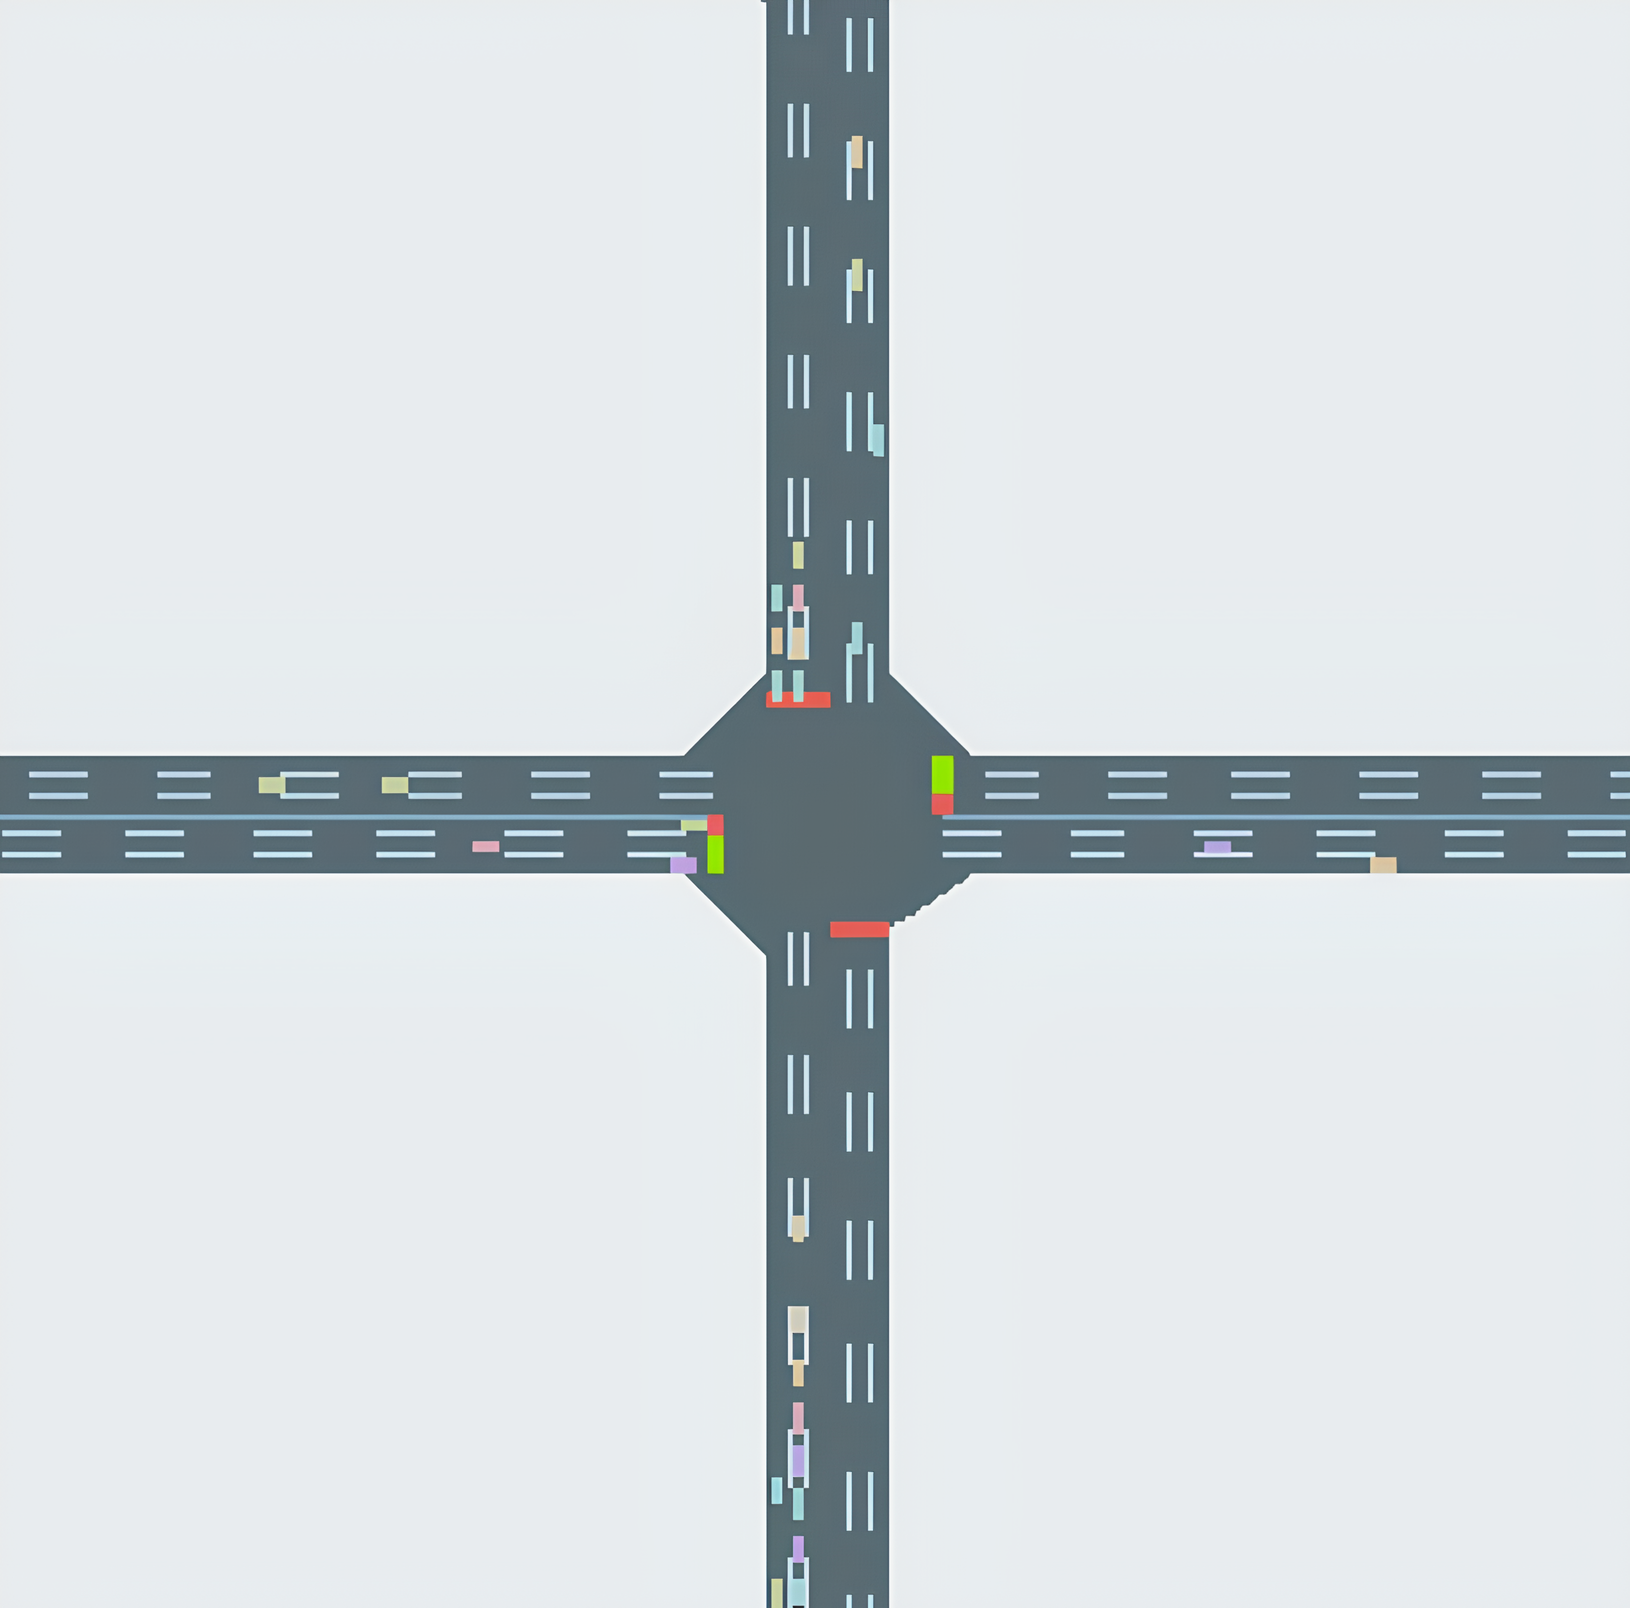
\includegraphics[width=0.7\textwidth]{screenshot_cityflow.png}
  \caption{Rendering del visualizzatore di \textsc{CityFlow} per una singola
    intersezione a quattro vie: le indicazioni verde/rosso ai margini
    dell'incrocio mostrano i movimenti abilitati dalla fase corrente, i
    rettangoli colorati sulle corsie i veicoli in transito o in coda.}
  \label{fig:cityflow-screenshot}
\end{figure}

\subsection{Struttura della rete e mappatura delle fasi}

La topologia della rete è codificata in un file di configurazione (\emph{roadnet}),
che definisce l'insieme delle intersezioni (nodi) e dei segmenti stradali (archi) con le relative molteplicità di corsia.
Per ogni intersezione il \emph{roadnet} elenca le fasi semaforiche disponibili, ciascuna definita
come l'insieme dei movimenti (coppie corsia di origine e di destinazione) abilitati in quella fase.
L'azione dell'agente si riduce pertanto alla selezione dell'indice corrispondente alla fase da attivare.
Ogni intersezione di questo lavoro modella 12 corsie in ingresso
(quattro direzioni cardinali, tre corsie ciascuna: sinistra, diritto, destra) e
8 fasi semaforiche selezionabili.
La Tabella~\ref{tab:fasi} riporta la mappatura di tali fasi (Figura~\ref{fig:fasi}), adottando la
nomenclatura N/S/E/W (\emph{North/South/East/West}) e T/L (\emph{Through}, diritto, e \emph{Left}, sinistra).

\begin{table}[htbp]
  \centering
  \small
  \begin{tabular}{@{}clp{7.5cm}@{}}
    \toprule
    Fase & Nome & Movimenti abilitati                      \\
    \midrule
    0    & NTST & Nord diritto+destra, Sud diritto+destra  \\
    1    & NLSL & Nord sinistra, Sud sinistra              \\
    2    & NTNL & Nord sinistra+diritto+destra             \\
    3    & STSL & Sud sinistra+diritto+destra              \\
    4    & WTET & Ovest diritto+destra, Est diritto+destra \\
    5    & WLEL & Ovest sinistra, Est sinistra             \\
    6    & ETEL & Est sinistra+diritto+destra              \\
    7    & WTWL & Ovest sinistra+diritto+destra            \\
    \bottomrule
  \end{tabular}
  \caption{Le 8 fasi semaforiche e i movimenti che ciascuna abilita.}
  \label{tab:fasi}
\end{table}

\begin{figure}[htbp]
  \centering
  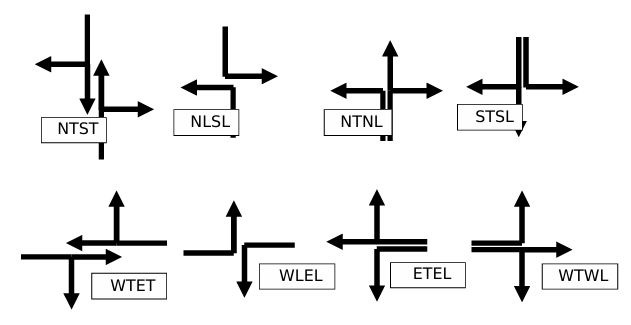
\includegraphics[width=0.85\textwidth]{fasi_semaforiche.png}
  \caption{Rappresentazione grafica delle 8 fasi di Tabella~\ref{tab:fasi}:
    le frecce indicano i movimenti abilitati da ciascuna fase.}
  \label{fig:fasi}
\end{figure}

Il riferimento originale permette ai veicoli che svoltano a destra di muoversi liberamente, senza attendere il semaforo verde, a patto che non vi siano veicoli provenienti da altre direzioni.
Al fine di prevenire una qualunque possibile interferenza tra diversi flussi e garantire un controllo più rigoroso, si è deciso di non adottare questo comportamento, permettendo la svolta a destra solo quando esplicitamente autorizzata dalla fase semaforica.
L'insieme delle fasi sopra riportate rappresenta una configurazione tale da sfruttare al massimo lo spazio delle direzioni possibili,
evitando al contempo conflitti tra le traiettorie dei veicoli.

\subsection{Gestione dell'interverde}
\label{subsec:interverde}

L'interverde è il periodo di tempo che intercorre tra la fine del verde di una fase semaforica
e l'inizio del verde di quella successiva.
Il suo scopo è quello di garantire la sicurezza stradale, permettendo ai veicoli che si trovano nell'intersezione di
sgombrarla prima che venga attivata la fase successiva.
Il motore di simulazione \textsc{CityFlow} non modella nativamente tale fase transitoria, nello specifico, non gestisce i semafori gialli e il conseguente passaggio sicuro tra due fasi consecutive;
dunque l'interverde deve essere costruito esplicitamente.
In questo lavoro, l'intervallo decisionale dell'agente (lo \emph{step} di simulazione) ha una durata complessiva $\Delta t_{\text{step}} = 15 \text{ s}$ simulati,
idealmente ripartita in tre sotto-fasi, con le stesse durate del riferimento originale:
verde ($\Delta t_{\text{green}} = 10 \text{ s}$), giallo ($\Delta t_{\text{yellow}} = 3 \text{ s}$) e "tutto-rosso" ($\Delta t_{\text{red}} = 2 \text{ s}$).
Per il limite di \textsc{CityFlow} sopra descritto e in questo studio accettato come compromesso, l'ambiente assimila il giallo al verde senza imporre modelli di decelerazione specifici,
mantenendo pertanto i movimenti autorizzati dalla policy per una durata totale di  $\Delta t_{\text{green}}+\Delta t_{\text{yellow}} = 13 \text{ s}$ consecutivi.
Al termine di questa finestra temporale, viene eseguita per $\Delta t_{\text{red}} = 2 \text{ s}$ una fase che non è presente tra le azioni selezionabili dal modello,
ovvero il semaforo rosso in contemporanea su tutte le corsie. Questo
intervallo di tutto-rosso viene eseguito a ogni step, indipendentemente
dal fatto che la fase successiva coincida o meno con quella corrente: anche
selezionare due volte di fila la stessa fase comporta i 2 s di
tutto-rosso.
Questo intervallo di guardia è necessario per garantire lo svuotamento dell'intersezione prima del cambio di fase, così da prevenire collisioni.
A questo punto lo step giunge al termine e il modello formula una nuova decisione, scegliendo quale delle 8 fasi implementare nel ciclo successivo.

È importante sottolineare che questa accortezza riduce di fatto il tempo effettivo utile di decisione del singolo agente di controllo semaforico, in quanto due dei quindici secondi di ogni step sono
dedicati alla fase "tutto-rosso" e quindi da considerarsi tempo morto (rappresentando circa il 13\% del tempo totale).

\subsection{Dataset e generazione parametrica}
\label{subsec:dataset}

Ogni roadnet e ogni flusso di traffico usato in questo lavoro è generato
parametricamente e in modo interamente deterministico da uno script dedicato,
senza alcun campionamento empirico.
Questo approccio consente di avere un pieno controllo sulle variabili operative come la
struttura della rete, la densità veicolare e presenza di arterie principali, oltre a
garantire l'esatta riproducibilità degli scenari di simulazione, un requisito metodologico fondamentale
per un equo confronto tra modelli di controllo semaforico.

\paragraph{Topologie e spaziature.}
L'ambiente di simulazione implementa tre topologie a griglia regolare di dimensioni $4\times4$ (16 intersezioni),
$5\times5$ (25 intersezioni) e $6\times6$ (36 intersezioni), impiegate per l'addestramento e per valutare la capacità di generalizzazione
dei modelli rispetto alla scala spaziale.

Un aspetto rilevante nella scelta della spaziatura tra incroci è la
comparsa spontanea della cosiddetta onda verde, uno standard strutturale
nell'ingegneria del traffico contemporanea: un flusso di veicoli che si
propaga attraverso la rete senza fermarsi ai semafori. La spaziatura tra
incroci è pertanto di due tipi: calibrata per l'onda verde e non
calibrata. In assenza di offset temporali, in quanto le transizioni di
fase sono sincrone per tutti i nodi della rete, l'unico modo per ottenere
un'onda verde è calibrare la distanza fisica tra gli incroci sulla
velocità di marcia e sulla durata del ciclo: alla velocità di riferimento
$v_{\max} = 11.1 \text{ m/s}$, in un ciclo di $\Delta t_{\text{step}} = 15
  \text{ s}$ viene percorsa una distanza pari a $166.5 \text{ m}$. Dunque
la prima spaziatura proposta è proprio di questa misura, ma ne faremo
riferimento con l'etichetta "100m". La spaziatura non calibrata invece è
100m più estesa e viene indicata con "200m".

Le roadnet non condividono tutte lo stesso ruolo. La griglia $4\times4$ con spaziatura "100m" compare sia in training sia in test,
mentre le altre tre combinazioni topologia-spaziatura restano riservate esclusivamente al test e non vengono mai incontrate durante l'addestramento
(Tabella~\ref{tab:roadnet-uso}). Questa separazione serve a isolare due assi di generalizzazione: le griglie $5\times5$ e $6\times6$ misurano la tenuta
della policy su reti più estese di quella di addestramento, con più intersezioni da coordinare, mentre la spaziatura "200m" applicata alla griglia $4\times4$
misura la tenuta su una topologia mai vista con incroci più distanziati, priva della calibrazione per l'onda verde descritta sopra.

\begin{table}[htbp]
  \centering
  \small
  \begin{tabular}{@{}llc@{}}
    \toprule
    Griglia    & Spaziatura & Utilizzo                \\
    \midrule
    $4\times4$ & 100m       & Train, Validation, Test \\
    $4\times4$ & 200m       & Test                    \\
    $5\times5$ & 100m       & Test                    \\
    $6\times6$ & 100m       & Test                    \\
    \bottomrule
  \end{tabular}
  \caption{Utilizzo di ciascuna combinazione topologia-spaziatura. Il dettaglio del confine tra training e validazione sulla griglia $4\times4$ a 100m è in Tabella~\ref{tab:split}.}
  \label{tab:roadnet-uso}
\end{table}

\begin{figure}[htbp]
  \centering
  \begin{subfigure}[t]{0.48\textwidth}
    \centering
    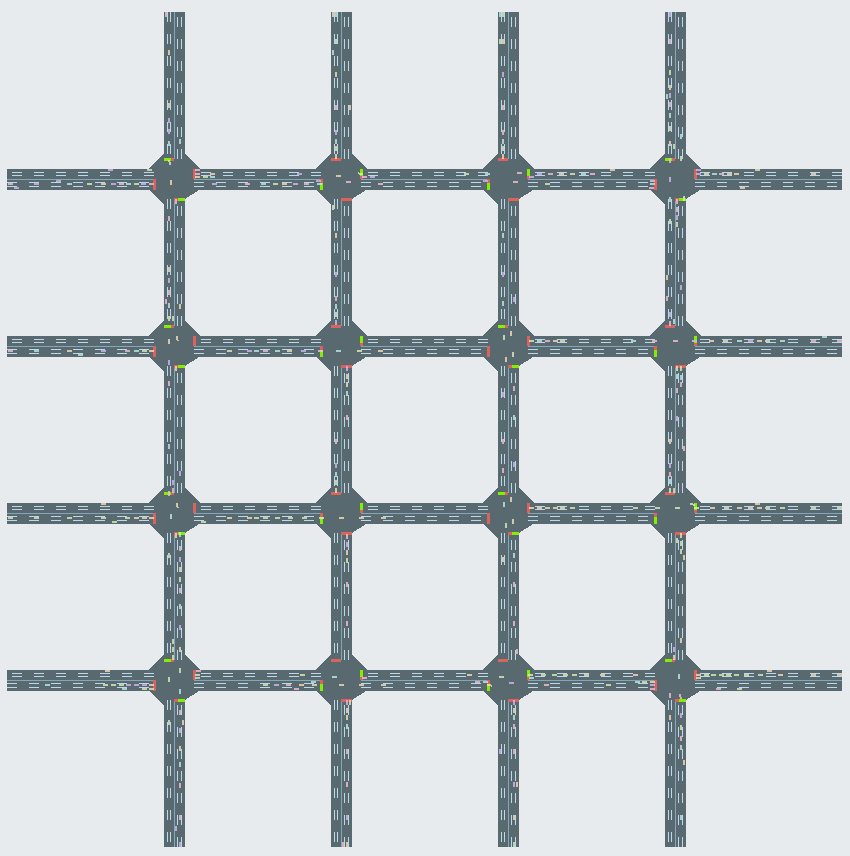
\includegraphics[width=\linewidth]{rete4x4.png}
    \caption{$4\times4$, 100m}
  \end{subfigure}
  \hfill
  \begin{subfigure}[t]{0.48\textwidth}
    \centering
    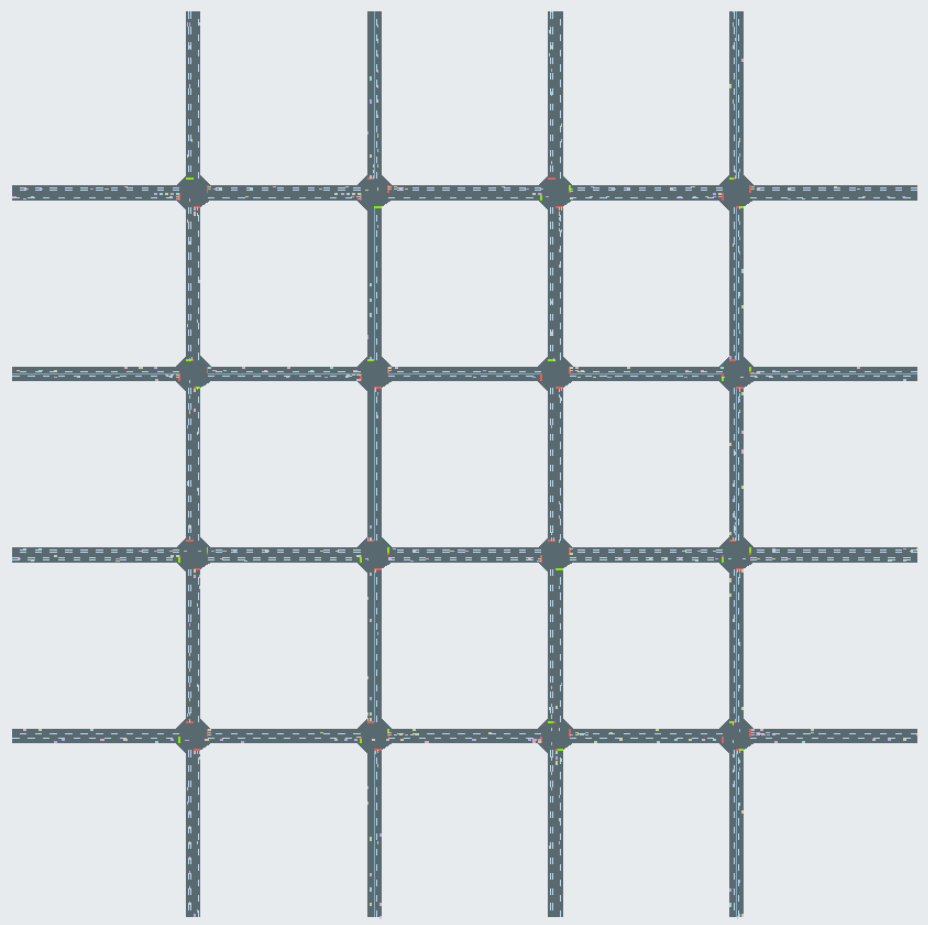
\includegraphics[width=\linewidth]{rete4x4_200m.png}
    \caption{$4\times4$, 200m}
  \end{subfigure}
  \par\bigskip
  \begin{subfigure}[t]{0.48\textwidth}
    \centering
    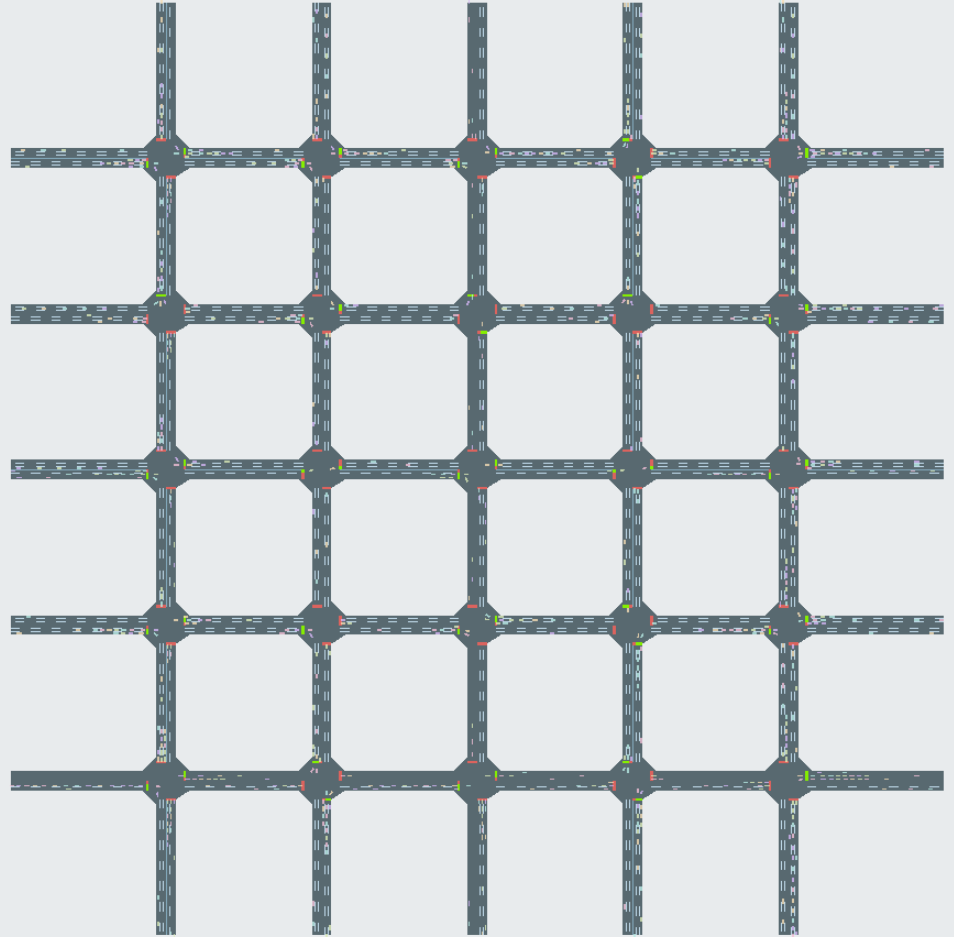
\includegraphics[width=\linewidth]{rete5x5.png}
    \caption{$5\times5$, 100m}
  \end{subfigure}
  \hfill
  \begin{subfigure}[t]{0.48\textwidth}
    \centering
    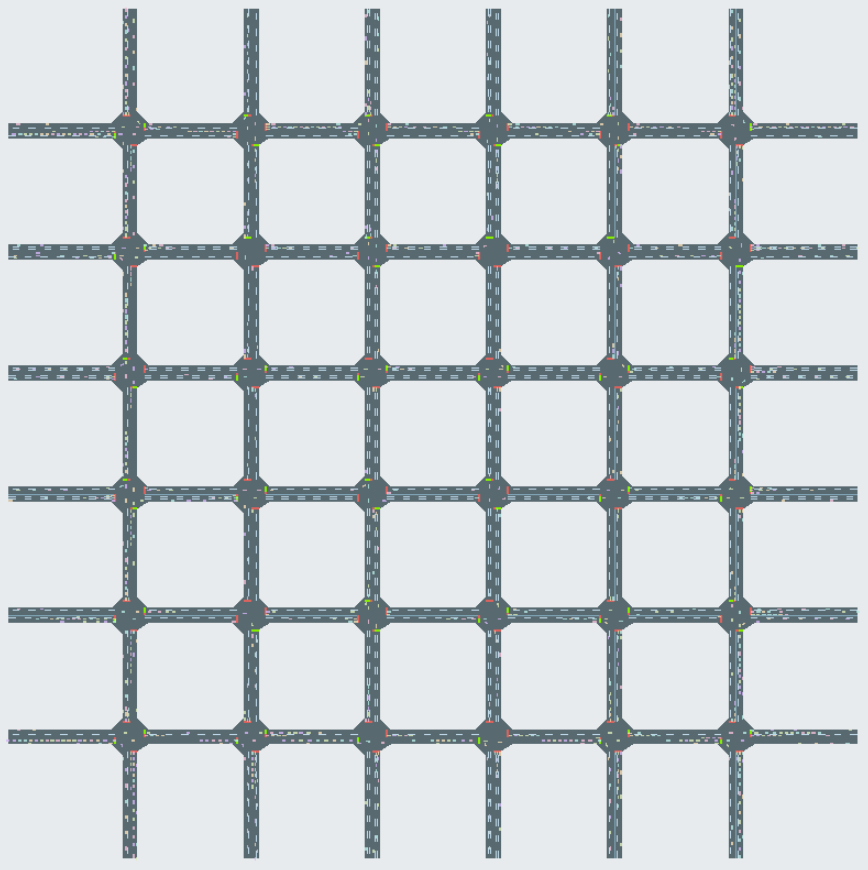
\includegraphics[width=\linewidth]{rete6x6.png}
    \caption{$6\times6$, 100m}
  \end{subfigure}
  \caption{Rendering nel visualizzatore di \textsc{CityFlow} delle quattro combinazioni topologia-spaziatura di Tabella~\ref{tab:roadnet-uso}.}
  \label{fig:roadnet-render}
\end{figure}

\paragraph{Percorsi veicolari.}
Il percorso di ciascun veicolo attraverso la rete non è fissato a priori, ma
generato casualmente per ciascun punto di ingresso sul perimetro della
griglia: a ogni incrocio attraversato, il percorso prosegue dritto con
probabilità $0.60$, svolta a destra con probabilità $0.30$ o svolta a
sinistra con probabilità $0.10$, finché non esce dai confini della rete o
non ripercorrerebbe un incrocio già attraversato (evitando così percorsi
ciclici). La probabilità complessiva di un percorso è il prodotto delle
probabilità delle singole scelte che lo compongono; il
numero di veicoli assegnato a ciascun percorso è proporzionale al suo peso relativo
sul totale dei percorsi generati da quel punto di ingresso, calibrato per
raggiungere il volume di traffico target di ciascuna fascia
(Tabella~\ref{tab:workday}).

\paragraph{Profili di traffico.}
Per ciascuna topologia sono stati generati tre profili di traffico:
un flusso a intensità costante (\emph{flat}),
un profilo a gradino (\emph{peak}, diviso in tre fasi temporali con un raddoppio del carico nel terzo centrale) e
un profilo dinamico (\emph{complete}) che simula il traffico di una giornata lavorativa (dettagliato nel seguito), impiegato esclusivamente in fase di addestramento.
Ogni episodio ha una durata di $T_{\text{max}} = 1800 \text{ s}$ simulati, corrispondenti a $1800 \text{ s} / \Delta t_{\text{step}} = 120$ cicli decisionali per agente.

I volumi dei veicoli immessi nella rete per ciascuna configurazione topologica sono stati determinati tramite una calibrazione empirica, così da garantire un livello
di saturazione comparabile tra reti di dimensioni diverse e quindi una difficoltà del task di controllo invariata rispetto la scala topologica.
In particolare la densità di ogni topologia è stata bilanciata affinché il \emph{trip completion} ottenuto dalla baseline \textsc{Max-Pressure} risultasse omogeneo ($90\%\text{--}94\%$).

\paragraph{Profilo di addestramento \emph{complete}.}
A differenza degli scenari di validazione e test, caratterizzati da densità costanti o a singolo picco,
il profilo di addestramento sintetizza l'evoluzione della domanda veicolare di un'intera giornata solare (24 ore) all'interno di un singolo episodio di $1800 \text{ s}$.
Come dettagliato nella Tabella~\ref{tab:workday}, il flusso è diviso in cinque fasce a intensità variabile:
due fasce a basso carico (assimilabili agli orari notturni),
due picchi di massima domanda (flussi di traffico di inizio e fine turno lavorativo) e
un intervallo di raccordo centrale a regime moderatamente sostenuto.
Questa marcata variazione di domanda veicolare all'interno di un singolo episodio è funzionale poiché costringe il modello ad adattare dinamicamente il piano di controllo,
senza convergere verso una policy specializzata soltanto su un unico flusso di traffico.

\begin{table}[htbp]
  \centering
  \small
  \begin{tabular}{@{}p{4.3cm}rrr@{}}
    \toprule
    Fascia     & Intervallo simulato & Step di decisione & Veicoli/secondo \\
    \midrule
    Flat basso & 0-525s              & 0-35              & 1.36            \\
    Peak basso & 525-675s            & 35-45             & 3.67            \\
    Flat alto  & 675-1200s           & 45-80             & 2.93            \\
    Peak alto  & 1200-1425s          & 80-95             & 4.78            \\
    Flat basso & 1425-1800s          & 95-120            & 1.27            \\
    \bottomrule
  \end{tabular}
  \caption{Le cinque fasce del profilo di addestramento \emph{complete}
    (totale: 4.728 veicoli per \texttt{train1}; \texttt{train2} e
    \texttt{train3} seguono la stessa struttura con lievi variazioni tra
    seed, per un totale rispettivamente di 4.723 e 4.620 veicoli).}
  \label{tab:workday}
\end{table}

\paragraph{Stocasticità e sbilanciamento direzionale.}
Per mitigare il rischio di \emph{overfitting} e garantire la robustezza del modello,
la generazione del profilo di addestramento integra due accorgimenti.

Innanzi tutto, considerata la natura deterministica di \textsc{CityFlow},
addestrare un modello su una singola configurazione esporrebbe l'agente all'apprendimento mnemonico di un'esatta sequenza di veicoli.
Per prevenire questa eventualità, si generano con diversi \emph{seed} tre profili di traffico differenti, in modo da perturbare
la distribuzione dei percorsi e gli istanti di immissione, pur mantenendo la medesima struttura generale descritta in Tabella~\ref{tab:workday};
tali varianti vengono quindi alternate ciclicamente durante l'addestramento.
Anche le configurazioni di validazione e test, su cui i modelli vengono valutati metodicamente, vengono generate con diversi \emph{seed} (5 per configurazione),
così da ottenere statistiche più robuste e informative sui risultati conseguiti.

In secondo luogo, per mettere alla prova la capacità del modello di adattarsi a situazioni locali di traffico differenti,
è stata indotta un'asimmetria direzionale, designando una riga orizzontale della griglia come arteria principale (Est-Ovest),
con un fattore di potenziamento di 3 che ne aumenta il peso nella distribuzione dei percorsi generati (senza alterare il volume totale di veicoli della configurazione).
Tale arteria viene posta su una riga diversa per ogni variante di addestramento, al fine di scongiurare l'ipotesi che le policy sviluppate siano dipendenti dalla posizione dell'incrocio,
mentre viene mantenuta fissa sulla stessa riga nelle configurazioni di validazione e di test, in modo da garantire la comparabilità dei risultati.

\paragraph{Training, validation e test.} La Tabella~\ref{tab:split}
raccoglie in un unico prospetto tutte le combinazioni di griglia, spaziatura
e profilo di traffico introdotte in questo lavoro, con il relativo utilizzo
nella pipeline sperimentale; le varianti seed di validazione e test sono
omesse, poiché non introducono combinazioni distinte da quelle elencate.
Le tre configurazioni di training compaiono anche nella batteria di test,
per un confronto diretto con la prassi, diffusa in letteratura, di
valutare un modello sulla stessa rete su cui è stato addestrato
(Capitolo~\ref{cap:confronto}). In tutto possiamo contare 11
configurazioni: 3 di training, 1 di validation e 7 di test.

\begin{table}[htbp]
  \centering
  \footnotesize
  \begin{tabular}{@{}lllll@{}}
    \toprule
    Griglia    & Spaziatura & Profilo di traffico       & Utilizzo    & Configurazione                          \\
    \midrule
    $4\times4$ & 100m       & Complete (arteria riga 0) & Train, Test & \texttt{config\_4x4\_100m\_train1}      \\
    $4\times4$ & 100m       & Complete (arteria riga 1) & Train, Test & \texttt{config\_4x4\_100m\_train2}      \\
    $4\times4$ & 100m       & Complete (arteria riga 2) & Train, Test & \texttt{config\_4x4\_100m\_train3}      \\
    $4\times4$ & 100m       & Flat                      & Validation  & \texttt{config\_4x4\_100m\_6k\_flat}    \\
    $4\times4$ & 100m       & Peak                      & Test        & \texttt{config\_4x4\_100m\_6k\_peak}    \\
    $4\times4$ & 200m       & Flat                      & Test        & \texttt{config\_4x4\_200m\_6k\_flat}    \\
    $4\times4$ & 200m       & Peak                      & Test        & \texttt{config\_4x4\_200m\_6k\_peak}    \\
    $5\times5$ & 100m       & Flat                      & Test        & \texttt{config\_5x5\_100m\_9.4k\_flat}  \\
    $5\times5$ & 100m       & Peak                      & Test        & \texttt{config\_5x5\_100m\_9.4k\_peak}  \\
    $6\times6$ & 100m       & Flat                      & Test        & \texttt{config\_6x6\_100m\_11.5k\_flat} \\
    $6\times6$ & 100m       & Peak                      & Test        & \texttt{config\_6x6\_100m\_11.5k\_peak} \\
    \bottomrule
  \end{tabular}
  \caption{Tutte le combinazioni di griglia, spaziatura e profilo di traffico impiegate in questo lavoro, a meno delle varianti seed di validazione e test, con il relativo utilizzo e il nome del file di configurazione corrispondente.}
  \label{tab:split}
\end{table}

\subsection{Assunzioni e limiti del modello di simulazione}
\label{subsec:assunzioni-simulazione}
Si esplicitano di seguito le semplificazioni strutturali adottate in fase di simulazione, finalizzate a ridurre la complessità computazionale e a rendere il problema trattabile:
\begin{itemize}
  \item \textbf{Fasi transitorie:} Come precedentemente illustrato, l'intervallo semaforico di giallo è assimilato cinematicamente a un prolungamento del verde.
        La prevenzione dei conflitti è affidata unicamente alla fase di "tutto-rosso".
  \item \textbf{Omogeneità topologica:} L'analisi è confinata a topologie a griglia regolare, con incroci ortogonali e segmenti stradali di lunghezza uniforme.
        Tale astrazione permette di isolare l'impatto della scala dimensionale e della spaziatura sulle prestazioni di generalizzazione, rimuovendo le distorsioni causate dalle irregolarità geometriche tipiche delle reti urbane reali.
  \item \textbf{Flusso unimodale e omogeneo:} La simulazione modella esclusivamente il traffico veicolare privato. Non sono previsti pedoni, ciclisti, trasporti pubblici o mezzi di soccorso.
        Inoltre, il flusso è perfettamente omogeneo: ogni veicolo condivide i medesimi parametri cinematici (dimensione, accelerazione massima, velocità massima).
  \item \textbf{Limiti di velocità uniformi:} Il limite di velocità $v_{\max}=11.1$ m/s è una costante globale, identica per ogni corsia della rete e per ogni veicolo generato, dunque sono assenti gerarchie stradali diverse.
  \item \textbf{Omogeneità degli incroci:} Ogni intersezione è vincolata a una geometria a quattro vie provvista di 8 fasi semaforiche, escludendo di fatto incroci con un numero diverso di vie.
  \item \textbf{Assenza di \emph{lane-changing}:} Le corsie in approccio sono dedicate in modo esclusivo ai singoli movimenti (svolta a sinistra, dritto, svolta a destra).
        I veicoli vengono generati e si immettono automaticamente nella corsia compatibile con il loro percorso e il cambio di corsia (\emph{lane-changing}) è una dinamica che non è stata implementata.
  \item \textbf{Viabilità bidirezionale:} L'infrastruttura di rete è composta esclusivamente da strade a doppio senso di marcia.
        La modellazione di strade a senso unico, per quanto frequente nei contesti urbani, non rientra nell'insieme delle configurazioni generate.
\end{itemize}

%!TEX root = ../mainufficiale.tex
\chapter{Esperimenti e risultati}
\label{cap:confronto}

Questo capitolo descrive il protocollo sperimentale di questa tesi e ne
riporta i risultati. Definisce anzitutto le metriche di valutazione
(§\ref{sec:metriche}) e il protocollo sperimentale
(§\ref{sec:protocollo}); presenta poi il confronto di base tra le
baseline classiche e MetaSTGAT Pro insieme ai tre studi sperimentali di
questa tesi, sul peso $\alpha$ della componente di equità, sull'ablation
della procedura di addestramento e sui meccanismi di comunicazione
spaziale alternativi (§\ref{sec:confronti}), e ne riporta i risultati
(§\ref{sec:risultati-baseline}).

\section{Metriche di valutazione}
\label{sec:metriche}

Nella letteratura sul Traffic Signal Control le metriche di valutazione
proposte sono numerose.
Questo capitolo introduce le 4 metriche principali utilizzate, coerentemente con il duplice obiettivo di
questo lavoro, ovvero efficienza ed equità (come motivato nel Capitolo~\ref{cap:introduzione}):
il \emph{travel time} (tempo di viaggio, medio e massimo) e il \emph{trip completion} (veicoli che
completano il percorso) per l'efficienza, il \emph{max wait} (l'attesa
massima registrata da un veicolo ad un incrocio) per l'equità.
C'è da sottolineare che né \emph{travel time} né
\emph{trip completion} sono metriche che appaiono esplicitamente nella
ricompensa dei modelli. Pertanto qualunque risultato su di esse sarà
l'indiretta conseguenza di come la reward ha indirizzato l'apprendimento
della policy.

\paragraph{Travel time.} Per ogni veicolo $v$, il tempo di viaggio è
\begin{equation}
  tt_v =
  \begin{cases}
    t_{\text{arrivo}}(v) - t_{\text{spawn}}(v)     & \text{se } v \text{ è arrivato entro la fine dell'episodio} \\
    t_{\text{fine episodio}} - t_{\text{spawn}}(v) & \text{altrimenti (un lower bound del vero valore)}
  \end{cases}
\end{equation}
Una delle due metriche cardine in questo studio è il travel time medio $\overline{tt}$,
ovvero la media di $ tt_v $ calcolata sull'intera popolazione di veicoli generati nell'episodio.
Tale metrica non considera soltanto i veicoli arrivati, ma include anche i
veicoli che non hanno completato il percorso entro la fine della simulazione.
La ragione è evitare un bias di sopravvivenza: un
modello che congestiona la rete e lascia arrivare solo una minoranza di
veicoli su percorsi ottimizzati otterrebbe, calcolando la media solo sui
veicoli arrivati, un risultato positivo ma non rappresentativo del comportamento reale della rete.

La seconda vera metrica cardine in questo lavoro di tesi è il travel time massimo $\overline{tt}_{\max}$,
ovvero il massimo tra tutti i travel time dei veicoli generati, anche in questo caso indipendentemente
dal completamento del percorso, per motivi analoghi a quelli descritti per il travel time medio.

\paragraph{Trip completion.} Questa metrica misura la percentuale di veicoli che hanno completato il percorso entro la
fine dell'episodio, escludendo dal totale i veicoli strutturalmente impossibilitati a farlo: quelli il cui tragitto, percorso a velocità massima costante e senza alcun arresto ai semafori, richiederebbe già da solo più dei secondi restanti alla fine dell'episodio a partire dal proprio istante di generazione.
Questo sottoinsieme dipende solo dallo scenario di traffico (percorso e istante di generazione di ciascun veicolo), non dal controllore, e viene quindi calcolato una sola volta per configurazione e riusato per ogni modello.
In questo studio questa metrica viene indicata con $tc$. Il dettaglio di
$tc$ per ogni singolo modello e ogni singola configurazione è in
Tabella~\ref{tab:tc-adjusted}, a fine capitolo.

\paragraph{Max wait.} Questa metrica riguarda il tempo più lungo che un
veicolo trascorre su una singola corsia del proprio percorso. Sia $w_v$
questo tempo per il veicolo $v$: l'intervallo tra l'istante in cui $v$
entra in una corsia del suo tragitto e quello in cui supera l'incrocio a
cui essa conduce, calcolato come il massimo su tutte le corsie
attraversate lungo il percorso. Il conteggio su una corsia non si azzera
se il veicolo avanza al suo interno, e prosegue anche se il veicolo si è
fermato e ripartito una o più volte prima di superare l'incrocio; si
interrompe soltanto quando la vettura lo supera. Il max wait
dell'episodio è
\begin{equation}
  \text{wait}_{\max} = \max_{v}\ w_v ,
\end{equation}
il massimo su tutti i veicoli generati nell'episodio.

Come per il travel time, include anche gli stalli ancora in corso al
termine dell'episodio. Sulle configurazioni con spaziatura di 200 metri
(§\ref{subsec:dataset}), il conteggio è esteso all'intera corsia invece di
limitarsi al campo visivo $d_{\text{vis}}$ dei modelli di reinforcement
learning (§\ref{sec:formalizzazione}): un veicolo fermo oltre $d_{\text{vis}}$
dal semaforo sarebbe altrimenti escluso dal computo, sottostimando l'attesa
peggiore effettivamente osservata sulla corsia.
In questo studio max wait viene indicato con $\text{wait}_{\max}$.

La presente metrica non va confusa con $\mathrm{MaxRedWait}_i^t$, il termine
usato nella ricompensa (Capitolo~\ref{cap:tsc-modelli}) per
penalizzare l'attesa durante il training. $\mathrm{MaxRedWait}_i^t$ è
calcolato a ogni singolo passo di decisione, su una sola intersezione alla
volta, ma soprattutto è limitata al campo visivo dell'incrocio.
$\text{wait}_{\max}$ è invece calcolato una sola volta a fine
episodio, come massimo su tutta la rete, e fa riferimento all'intera corsia.

\section{Protocollo sperimentale}
\label{sec:protocollo}

Ogni modello RL è addestrato sulle tre configurazioni di training presentate nella Tabella~\ref{tab:split}.

Seguendo un ciclo fisso, le tre configurazioni si alternano episodio per
episodio. A fine training, l'ultimo checkpoint e quello che ha ottenuto il
valore di loss più basso durante l'intero addestramento sono confrontati
sulla configurazione di validazione \texttt{config\_4x4\_100m\_6k\_flat},
mediando $\overline{tt}$ su 5 seed diversi.
Questa fase serve a evitare due problemi che si concatenano tra loro.
Il primo è che in un ciclo di
apprendimento online la politica non converge necessariamente in modo
monotono, dunque gli ultimi episodi addestrati potrebbero allontanare la policy da un
punto di minimo quantomeno locale.
Il secondo è che la scelta del modello che ha registrato la loss minima non garantisce
le capacità di generalizzazione del modello, in quanto una loss bassa potrebbe
anche essere sintomo di una policy che ha soltanto memorizzato delle condizioni particolari delle
configurazioni di training, senza però aver realmente appreso una politica in grado di generalizzare.

La selezione si basa sul solo $\overline{tt}$ e non sulle metriche di caso
peggiore che questo lavoro tiene in primo piano altrove: mediare il
travel time medio sui 5 seed di validazione dà già una stima
ragionevolmente stabile del checkpoint migliore, mentre fare lo stesso con
un massimo come $tt_{\max}$ o $\text{wait}_{\max}$ resterebbe una stima
molto più rumorosa, perché un massimo risente della coda della
distribuzione assai più di una media. È un limite pratico del protocollo,
non una scelta di principio.

Il modello che risulta essere migliore in questa fase di selezione, viene poi utilizzato nella fase di test.
Ogni valutazione, sia in validation sia nella batteria di test che descriveremo ora, avviene con $\varepsilon=0$:
nessuna esplorazione residua, solo la politica appresa allo stato puro. Inoltre i risultati ottenuti in ciascuna
configurazione testata, sono mediati su 5 seed diversi, analogamente a quanto fatto per $\overline{tt}$ nella fase di validazione.

Misurare la capacità di generalizzazione dei modelli è uno degli obiettivi
dichiarati di questo lavoro (Capitolo~\ref{cap:introduzione}), un asse che
gran parte della letteratura sul controllo semaforico appreso non copre
sistematicamente, in quanto la prassi più diffusa, seguita anche dall'articolo
originale di MetaSTGAT \citep{wang2022metastgat}, è addestrare e valutare un modello sulla stessa
rete stradale, senza mai trasferirlo a una topologia diversa.

Per questo motivo la batteria di test di questo lavoro include sia le 3
configurazioni di training sia 7 configurazioni aggiuntive mai viste
durante l'addestramento. Le prime permettono un confronto diretto con la
prassi di letteratura appena descritta, riportando un risultato ottenuto
nelle stesse condizioni con cui la maggior parte degli altri lavori
riporta il proprio; le seconde, assenti nella maggior parte degli studi
citati, misurano invece se le prestazioni osservate si confermano anche con il cambio
di topologia e di condizioni di traffico.

Ogni modello, RL o baseline, è dunque valutato sistematicamente sulle
stesse 10 configurazioni: le 3 varianti di training stesse (per misurare la
prestazione in-distribuzione) più 7 configurazioni mai viste in training
(4x4 a 100m con profilo \emph{peak}, 4x4 a 200m invece di 100m con densità sia
\emph{flat} sia \emph{peak}, $5\times5$ e $6\times6$ a densità sia
\emph{flat} sia \emph{peak}), usate per misurare la generalizzazione a
profili di traffico, spaziature e topologie mai incontrati in training.

Ogni modello di questo lavoro, RL o ablation, deriva da un singolo run di
addestramento. La batteria a più seed appena descritta ripete la sola
valutazione, non l'addestramento: le medie e le deviazioni standard
riportate in questo capitolo descrivono quindi la variabilità della
policy già addestrata su scenari di valutazione diversi, non la
variabilità tra run di addestramento indipendenti.

\section{Confronti proposti}
\label{sec:confronti}

Il confronto sperimentale di questo capitolo è organizzato in tre studi indipendenti,
ciascuno dei quali varia una sola dimensione (il peso $\alpha$, un gruppo di
modifiche alla procedura, il meccanismo spaziale) rispetto al
modello di riferimento ($\alpha=0.08$, MetaSTGAT a un layer) a cui ci riferiremo con il termine \emph{MetaSTGAT Pro},
lasciando invariato tutto il resto. Verranno analizzati nel seguito i tre studi proposti.
Ciascun confronto conterrà al suo interno, come riferimento, le due baseline classiche, Fixed-Time e Max-Pressure, e il modello \emph{MetaSTGAT Pro}.

\subsection{Studio del peso \texorpdfstring{$\alpha$}{alpha}}

Il primo studio (§\ref{sec:risultati-alpha}) pone a confronto tre varianti del
modello MetaSTGAT Pro che differiscono solo per il valore del peso $\alpha$ riguardante la penalità anti-starvation
nella ricompensa (Eq.~\ref{eq:reward-custom}).
In particolare vengono valutati i valori di $\alpha \in \{0.08, 0.04, 0.00\}$.
È il confronto più diretto per quantificare il compromesso tra efficienza ed
equità dichiarato come obiettivo di questo lavoro.
Variando solo questo iperparametro della ricompensa, senza toccare stato o architettura,
osserveremo quanto costa in termini di travel time medio ottenere una data riduzione del travel time massimo e del max wait.

\subsection{Studio di ablazione}

Il secondo confronto (§\ref{sec:ablation-risultati}) isola sistematicamente ogni blocco di differenze
tra l'implementazione di questo lavoro e la procedura
descritta nell'articolo originale di MetaSTGAT, tramite 6 preset che
vanno dalla replica fedele del paper al modello MetaSTGAT Pro.
È un confronto necessario perché né l'uno né l'altro estremo, da soli,
spiegano il divario di prestazioni osservato tra i due: isolare un
sottosistema alla volta permette di valutare il contributo di ciascuna modifica.

Ogni preset applica un gruppo coerente di scelte configurative,
isolando un sottosistema alla volta rispetto al modello MetaSTGAT Pro (§\ref{subsec:framing-pro}):

\begin{table}[htbp]
  \centering
  \small
  \begin{tabular}{@{}llp{8.5cm}@{}}
    \toprule
    Preset                   & Reward          & Cosa isola rispetto a Pro                                            \\
    \midrule
    \texttt{pro}             & \texttt{custom} & --                                                                   \\
    \texttt{temporal}        & \texttt{custom} & burn-in + BPTT sulla Meta-LSTM                                       \\
    \texttt{single\_dqn}     & \texttt{custom} & Double DQN                                                           \\
    \texttt{vanilla\_buffer} & \texttt{custom} & PER, Huber, grad clipping, warm-up, esplorazione ciclica             \\
    \texttt{environment}     & \texttt{paper}  & campo visivo, feature dello stato $w_i^t$, maschera fasi consecutive \\
    \texttt{paper}           & \texttt{paper}  & Replica fedele di Wang et al. (2022)                                 \\
    \bottomrule
  \end{tabular}
  \caption{Preset di ablazione e sottosistema isolato da ciascuno. La reward \texttt{custom} è definita da Eq. (\ref{eq:reward-custom}), mentre la reward \texttt{paper} è definita da Eq. (\ref{eq:reward-paper}).}
  \label{tab:ablation-preset}
\end{table}

A differenza degli altri quattro preset, che modificano un solo sottosistema,
\texttt{environment} cambia contemporaneamente osservazione (campo visivo,
$w_i^t$, maschera) e ricompensa (torna a quella di Wang et al., 2022): i
suoi risultati misurano quindi l'effetto congiunto delle due cose, non
isolano un singolo meccanismo.

\subsection{Studio sui meccanismi spaziali}

Il terzo studio (§\ref{sec:confronto-spaziale}) sostituisce il solo
meccanismo di comunicazione spaziale tra intersezioni di MetaSTGAT Pro.
Vengono testate le seguenti varianti già introdotte nel Capitolo \ref{sec:spatial-alt}:
\begin{itemize}
  \item MetaSTGAT (il riferimento, a un layer come nella formulazione standard e a due layer)
  \item MetaSTGCN (a uno e due layer)
  \item MetaSTSONAR (con $L=2$ e $L=4$ iterazioni)
\end{itemize}

È il confronto che verifica se il beneficio osservato dipenda
specificamente dal meccanismo di attenzione appreso, o se una qualunque
forma di condivisione spaziale dell'informazione tra nodi vicini produca
risultati equivalenti.

\section{Risultati}
\label{sec:risultati-baseline}

I tre studi del precedente capitolo (§\ref{sec:confronti}) sono presentati
secondo uno schema comune: una tabella mediata sulle 3 configurazioni di
training, una corrispondente sulle 7 di test, un grafico a bande sovrapposte che le
riassume visivamente, un plot della variazione percentuale delle metriche principali rispetto a
Max-Pressure, gli eventuali casi particolari osservabili solo scendendo
alla singola configurazione, chiusi da una discussione che include, dove il risultato non
era quello atteso, una possibile spiegazione.
In queste tabelle, dallo studio sul peso $\alpha$ in poi, sono evidenziati
in grassetto i due risultati migliori di ogni colonna; nelle due tabelle
del confronto di base (§\ref{sec:risultati-base}), che hanno solo tre
righe, resta invece in grassetto il solo valore migliore.

Fixed-Time, Max-Pressure e MetaSTGAT Pro ($\alpha=0.08$, il modello di
riferimento di questo lavoro) compaiono in ciascuno dei tre studi.
Dunque, per non ripetere la stessa discussione su questi tre riferimenti di base,
la sottosezione seguente li confronta da soli,
mentre le sottosezioni successive approfondiranno i rispettivi confronti
(peso $\alpha$, ablazione, meccanismi spaziali).

\subsection{Fixed-Time, Max-Pressure e Pro: il confronto di base}
\label{sec:risultati-base}

\begin{table}[htbp]
  \centering
  \begin{tabular}{@{}lrrrr@{}}
    \toprule
    Modello                       & $\overline{tt}$ (s) & $tt_{\max}$ (s) & wait$_{\max}$ (s) & $tc$ $(\%)$   \\
    \midrule
    Fixed-Time                    & 339.3               & 1030.0          & 935.0             & 86.2          \\
    Max-Pressure                  & \textbf{161.9}      & 1070.0          & 1040.0            & \textbf{97.9} \\
    MetaSTGAT Pro ($\alpha=0.08$) & 172.8               & \textbf{630.0}  & \textbf{425.0}    & 97.4          \\
    \bottomrule
  \end{tabular}
  \caption{Travel time medio, massimo, max wait e trip completion dei tre
    controllori presenti in ogni studio di questo capitolo, mediati sulle 3
    configurazioni di training.}
  \label{tab:base-train}
\end{table}

\begin{table}[htbp]
  \centering
  \begin{tabular}{@{}lrrrr@{}}
    \toprule
    Modello                       & $\overline{tt}$ (s) & $tt_{\max}$ (s) & wait$_{\max}$ (s) & $tc$ $(\%)$   \\
    \midrule
    Fixed-Time                    & 460.7               & 1496.1          & 1311.0            & 84.0          \\
    Max-Pressure                  & \textbf{238.3}      & 1647.4          & 1636.7            & 91.9          \\
    MetaSTGAT Pro ($\alpha=0.08$) & 241.0               & \textbf{1017.4} & \textbf{792.0}    & \textbf{93.8} \\
    \bottomrule
  \end{tabular}
  \caption{Come Tabella~\ref{tab:base-train}, mediata sulle 7 configurazioni
    di test.}
  \label{tab:base-test}
\end{table}

Fixed-Time è il controllore peggiore su travel time medio e su trip
completion, in entrambi i regimi. Il quadro si inverte però su
$tt_{\max}$ e $wait_{\max}$: Max-Pressure non batte Fixed-Time su nessuna
delle due metriche, né in training ($tt_{\max}$ 1070.0s contro 1030.0s,
$wait_{\max}$ 1040.0s contro 935.0s) né in test (1647.4s contro 1496.1s,
1636.7s contro 1311.0s). Una spiegazione plausibile è strutturale:
Max-Pressure sceglie a ogni istante la fase che libera più veicoli, senza
mai considerare da quanto tempo attende la direzione esclusa
(Capitolo~\ref{cap:introduzione}), e può quindi in linea di principio far
attendere a lungo una direzione a bassa pressione se le altre restano
sempre più cariche; la rotazione fissa di Fixed-Time, per quanto cieca al
traffico reale, garantisce invece per costruzione che ogni fase torni
periodicamente, ponendo un limite strutturale all'attesa massima che una
regola puramente reattiva non ha. MetaSTGAT Pro resta l'unico dei tre a
battere Fixed-Time su ogni metrica, in entrambi i regimi. Non osservando
mai lo stato della rete, Fixed-Time resta comunque il riferimento più
semplice rispetto a cui ogni strategia reattiva o appresa può essere
confrontata.

Tra Max-Pressure e MetaSTGAT Pro il confronto è più sfumato. In training e in test Max-Pressure
resta il modello con il travel time medio più basso in assoluto (rispettivamente 161.9s e 238.3s),
coerente con la sua ottimalità di portata a livello di rete;
MetaSTGAT Pro paga per questo un travel time leggermente peggiore sia in training (172.8s, +6.7\%) sia in test (241.0s, +1.1\%).
Un'eccezione a questo quadro emerge scendendo alle singole configurazioni
di test: sulle due griglie $6\times6$, le più estese testate e mai viste
in training, MetaSTGAT Pro registra un travel time medio inferiore a
quello di Max-Pressure (238.1s contro 244.7s in \emph{flat}, 275.1s contro
283.3s in \emph{peak}), l'unico caso tra le 10 configurazioni in cui questo
avviene. Lo stesso pattern, sulle stesse due configurazioni, si osserva
anche per $\alpha=0.04$ e per \texttt{vanilla\_buffer}
(§\ref{sec:ablation-risultati}), il che rende meno probabile si tratti di
rumore. Una spiegazione plausibile è che, sulla rete più estesa e mai
vista in training, il coordinamento appreso tra intersezioni inizi a
incidere anche sull'efficienza media, mentre Max-Pressure, privo di
qualunque nozione della rete oltre l'incrocio corrente, perda parte del
proprio vantaggio quando la rete cresce oltre la scala di training; questo
lavoro non arriva a verificare se il divario continui a crescere su reti
ancora più estese.
Per quanto riguarda il $wait_{\max}$ il rapporto si inverte nettamente:
MetaSTGAT Pro registra un valore il 59\% più basso di Max-Pressure in training e il 52\% più basso in test
(Tabelle~\ref{tab:base-train}-\ref{tab:base-test}).
Questi risultati introducono il compromesso al centro di questo lavoro, discusso nella sua forma
completa al variare di $\alpha$ nella prossima sottosezione.
Il vantaggio relativo di MetaSTGAT Pro sul $wait_{\max}$ di Max-Pressure è
più ampio in training (59\%) che in test (52\%); una lettura cauta è che
parte di questo vantaggio si eroda, come atteso, su condizioni mai
incontrate in addestramento, senza che questo permetta di per sé
conclusioni più forti sulle capacità di generalizzazione del modello.

Sul completamento ($tc$) la separazione più netta è quella tra Fixed-Time
e tutti gli altri modelli di questo capitolo: 86.2\%/84.0\%
(training/test) contro un intervallo compreso tra il 94.4\% e il 97.9\% in
training e tra l'89.0\% e il 95.8\% in test per ogni altra variante
(Tabella~\ref{tab:tc-adjusted}, a fine capitolo); l'unica
eccezione parziale è MetaSTGCN, il cui completamento più basso è discusso
a parte in §\ref{sec:confronto-spaziale}. Tra Max-Pressure e MetaSTGAT
Pro, quest'ultimo ottiene un $tc$ più alto su tutte e 7 le configurazioni
di test, un vantaggio sistematico non limitato alle due griglie
$6\times6$ già osservate sul travel time medio. Con questo unico scarto
rilevante già osservato qui, le sottosezioni seguenti non ripetono la
discussione di $tc$ configurazione per configurazione: si limitano a
segnalarne la tendenza generale, rimandando alla stessa tabella per il
dettaglio completo.

\subsection{Studio del peso \texorpdfstring{$\alpha$}{alpha}: risultati}
\label{sec:risultati-alpha}
\label{sec:equita-alpha}

Questa sottosezione confronta i due controllori di riferimento
(§\ref{sec:risultati-base}) con le tre varianti del modello Pro che
differiscono solo per il peso $\alpha$ della penalità anti-starvation,
con $\alpha \in \{0.08, 0.04, 0.00\}$.

\begin{table}[htbp]
  \centering
  \begin{tabular}{@{}lrrr@{}}
    \toprule
    Modello                       & $\overline{tt}$ (s) & $tt_{\max}$ (s) & wait$_{\max}$ (s) \\
    \midrule
    Fixed-Time                    & 339.3               & 1030.0          & 935.0             \\
    Max-Pressure                  & \textbf{161.9}      & 1070.0          & 1040.0            \\
    MetaSTGAT Pro ($\alpha=0.08$) & 172.8               & \textbf{630.0}  & \textbf{425.0}    \\
    MetaSTGAT Pro ($\alpha=0.04$) & \textbf{170.7}      & \textbf{685.0}  & 560.0             \\
    MetaSTGAT Pro ($\alpha=0.00$) & 173.5               & 740.0           & \textbf{555.0}    \\
    \bottomrule
  \end{tabular}
  \caption{Travel time medio, massimo e max wait, mediati
    sulle 3 configurazioni di training.}
  \label{tab:risultati-train}
\end{table}

\begin{table}[htbp]
  \centering
  \begin{tabular}{@{}lrrr@{}}
    \toprule
    Modello                       & $\overline{tt}$ (s) & $tt_{\max}$ (s) & wait$_{\max}$ (s) \\
    \midrule
    Fixed-Time                    & 460.7               & 1496.1          & 1311.0            \\
    Max-Pressure                  & \textbf{238.3}      & 1647.4          & 1636.7            \\
    MetaSTGAT Pro ($\alpha=0.08$) & \textbf{241.0}      & \textbf{1017.4} & \textbf{792.0}    \\
    MetaSTGAT Pro ($\alpha=0.04$) & 241.1               & \textbf{1054.7} & \textbf{930.9}    \\
    MetaSTGAT Pro ($\alpha=0.00$) & 247.5               & 1164.4          & 1012.3            \\
    \bottomrule
  \end{tabular}
  \caption{Come Tabella~\ref{tab:risultati-train}, mediata sulle 7
    configurazioni di test.}
  \label{tab:risultati-test}
\end{table}

Sul travel time medio ciò che verrebbe naturale attendersi è che
al crescere del valore di $\alpha$ la metrica in questione peggiori, con
le due configurazioni prive di penalità anti-starvation, Max-Pressure e $\alpha=0.00$, che risulterebbero essere le
migliori, in quanto nessuna delle due paga un compromesso con l'equità, quindi
nessuna dovrebbe peggiorare travel time medio in cambio di un vantaggio che non
persegue.
I dati non confermano questa attesa in modo netto: $\alpha=0.00$ non è la
variante Pro con il travel time medio più basso, né in training né in
test (173.5s in training contro 172.8s di $\alpha=0.08$ e 170.7s di
$\alpha=0.04$; 247.5s in test contro 241.0s e 241.1s), ma il distacco dalle
altre due varianti non è sistematico come atteso. Una
causa plausibile: con
$\alpha=0$ il termine di ricompensa legato all'attesa scompare, ma il
vettore $w_i^t$ resta nello stato osservato dalla rete
(§\ref{sec:formalizzazione}); la rete continua quindi a vedere un segnale
che la ricompensa non penalizza più, un disallineamento tra stato e
obiettivo che può disturbare l'addestramento.

Tra le tre varianti Pro, $\alpha=0.04$ resta quella con il travel time
medio più basso in training (170.7s), pur restando dietro a Max-Pressure
in entrambi i regimi.

\begin{figure}[htbp]
  \centering
  \begin{subfigure}[t]{0.48\textwidth}
    \centering
    \includegraphics[width=\linewidth]{pro_alpha_train.png}
    \caption{Configurazioni di training}
  \end{subfigure}
  \hfill
  \begin{subfigure}[t]{0.48\textwidth}
    \centering
    \includegraphics[width=\linewidth]{pro_alpha_test.png}
    \caption{Configurazioni di test}
  \end{subfigure}
  \caption{Travel time medio (fascia scura), max wait (fascia intermedia) e
    travel time massimo (fascia chiara) per lo studio sistematico su $\alpha$, stessi dati
    delle Tabelle~\ref{tab:risultati-train}-\ref{tab:risultati-test}.}
  \label{fig:overlay-pro-alpha}
\end{figure}

\begin{figure}[htbp]
  \centering
  \begin{subfigure}[t]{0.48\textwidth}
    \centering
    \includegraphics[width=\linewidth]{diff_pct_alpha_train.png}
    \caption{Configurazioni di training}
  \end{subfigure}
  \hfill
  \begin{subfigure}[t]{0.48\textwidth}
    \centering
    \includegraphics[width=\linewidth]{diff_pct_alpha_test.png}
    \caption{Configurazioni di test}
  \end{subfigure}
  \caption{Variazione percentuale di travel time medio e massimo rispetto a
    Max-Pressure (riferimento a 0\%) per lo studio su $\alpha$, calcolata per
    singola configurazione e poi mediata.}
  \label{fig:diffpct-alpha}
\end{figure}

Su $tt_{\max}$ il quadro è quello atteso: la metrica peggiora in modo
strettamente monotono al diminuire di $\alpha$, cioè al ridursi del peso
dato al caso di starvation più estremo, in entrambi i regimi. Su
$wait_{\max}$ l'andamento è quasi monotono: in test $\alpha=0.00$ (1012.3s)
resta peggiore di $\alpha=0.04$ (930.9s) come atteso, ma in training i due
valori sono sostanzialmente pari (555.0s contro 560.0s): le configurazioni
di training, a differenza di quelle di test, non sono mediate su più
seed, per cui una differenza di 5 secondi tra le due non è distinguibile
da una singola realizzazione senza una stima della variabilità a
supporto. Il
riferimento $\alpha=0.08$ ottiene comunque sia il $tt_{\max}$ sia il
$wait_{\max}$ più bassi in entrambi i regimi, il 59\% in meno
di Max-Pressure in training e il 52\% in meno in test. In test sia $\alpha=0.04$
sia $\alpha=0.00$ restano nettamente sotto Fixed-Time su entrambe le metriche
($wait_{\max}$ rispettivamente 930.9s e 1012.3s, $tt_{\max}$ 1054.7s e 1164.4s,
contro 1311.0s e 1496.1s di Fixed-Time): rimuovere del tutto la
penalità anti-starvation non avvicina le prestazioni di caso peggiore
a quelle di un controllo non adattivo.

Nonostante il lieve vantaggio di $\alpha=0.04$ sul travel time medio in
training, il resto di questo lavoro adotta $\alpha=0.08$ come riferimento
standard per gli studi di ablazione e dei meccanismi spaziali
(§\ref{sec:ablation-risultati}, §\ref{sec:confronto-spaziale}). La ragione
è la priorità dichiarata tra le metriche di questo lavoro:
$\alpha=0.04$ è sistematicamente meno incisivo di
$\alpha=0.08$ su $wait_{\max}$ e $tt_{\max}$, le due metriche di caso peggiore
che questa tesi tiene in primo piano, a fronte di un guadagno sul solo
travel time medio, la meno critica delle tre e comunque assente in test.
$\alpha=0.08$ resta quindi
la scelta più coerente con l'obiettivo del lavoro, anche al costo di
qualche secondo in più di travel time medio.

\subsection{Studio di ablazione: risultati}
\label{sec:ablation-risultati}

Questa sottosezione confronta il modello Pro ($\alpha=0.08$, riferimento)
con i cinque preset di ablation presenti nella Tabella~\ref{tab:ablation-preset}:
\texttt{paper} (replica fedele del riferimento originale), \texttt{environment}
(campo di visibilità, $w_i^t$ e maschera azioni rimossi),
\texttt{temporal} (burn-in e BPTT disattivati), \texttt{single\_dqn}
(Double DQN sostituita da DQN) e \texttt{vanilla\_buffer} (PER, Huber,
gradient clipping, warm-up ed esplorazione ciclica disattivati),
tutti allo stesso $\alpha=0.08$ del riferimento.

\begin{table}[htbp]
  \centering
  \begin{tabular}{@{}lrrr@{}}
    \toprule
    Modello                          & $\overline{tt}$ (s) & $tt_{\max}$ (s) & wait$_{\max}$ (s) \\
    \midrule
    Fixed-Time                       & 339.3               & 1030.0          & 935.0             \\
    Max-Pressure                     & \textbf{161.9}      & 1070.0          & 1040.0            \\
    Pro ($\alpha=0.08$, riferimento) & 172.8               & \textbf{630.0}  & \textbf{425.0}    \\
    \texttt{paper}                   & 187.8               & 950.0           & 915.0             \\
    \texttt{environment}             & 188.3               & 1335.0          & 1290.0            \\
    \texttt{temporal}                & 176.0               & 715.0           & 560.0             \\
    \texttt{single\_dqn}             & 171.9               & \textbf{600.0}  & \textbf{485.0}    \\
    \texttt{vanilla\_buffer}         & \textbf{171.5}      & 695.0           & 560.0             \\
    \bottomrule
  \end{tabular}
  \caption{Travel time medio, massimo e max wait sui preset
    di ablazione, mediati sulle 3 configurazioni di training.}
  \label{tab:ablation-train}
\end{table}

\begin{table}[htbp]
  \centering
  \begin{tabular}{@{}lrrr@{}}
    \toprule
    Modello                          & $\overline{tt}$ (s) & $tt_{\max}$ (s) & wait$_{\max}$ (s) \\
    \midrule
    Fixed-Time                       & 460.7               & 1496.1          & 1311.0            \\
    Max-Pressure                     & \textbf{238.3}      & 1647.4          & 1636.7            \\
    Pro ($\alpha=0.08$, riferimento) & \textbf{241.0}      & \textbf{1017.4} & \textbf{792.0}    \\
    \texttt{paper}                   & 270.4               & 1553.6          & 1513.3            \\
    \texttt{environment}             & 268.6               & 1495.3          & 1463.1            \\
    \texttt{temporal}                & 245.9               & 1129.3          & 940.7             \\
    \texttt{single\_dqn}             & 243.2               & 1051.7          & 917.6             \\
    \texttt{vanilla\_buffer}         & 241.1               & \textbf{1044.9} & \textbf{804.0}    \\
    \bottomrule
  \end{tabular}
  \caption{Come Tabella~\ref{tab:ablation-train}, mediata sulle 7
    configurazioni di test.}
  \label{tab:ablation-test}
\end{table}

Sul travel time medio in training \texttt{vanilla\_buffer},
\texttt{single\_dqn} e il modello Pro restano in
una fascia stretta (171.5-172.8s), con \texttt{temporal} poco distante (176.0s);
\texttt{environment} se ne stacca già in questo regime (188.3s), non solo in test.
In test \texttt{vanilla\_buffer} e Pro restano quasi coincidenti (241.0-241.1s),
seguiti da \texttt{single\_dqn} (243.2s) e \texttt{temporal} (245.9s), mentre
\texttt{environment} e \texttt{paper} restano nettamente distanti (268.6s e 270.4s).
Il distacco di \texttt{environment} non è concentrato sulle due
configurazioni a 200m come si potrebbe attendere dalla sola disattivazione
del cutoff di visibilità: la variazione percentuale rispetto al riferimento
Pro, calcolata per singola configurazione, è di circa il 10\% sulle due
config a 200m e di circa il 12\% sulle restanti cinque config di test (4x4
a 100m, $5\times5$, $6\times6$), un divario distribuito in modo pressoché
uniforme su tutte le configurazioni fuori distribuzione, non specifico
della spaziatura. Questo rende meno convincente l'ipotesi che il solo
cutoff di visibilità sia responsabile del calo: \texttt{environment}
disattiva contemporaneamente anche $w_i^t$ nello stato, la maschera
anti-starvation e il termine di attesa nella ricompensa
(Tabella~\ref{tab:differenze}), e l'effetto osservato è più probabilmente
il risultato congiunto di queste rimozioni che di una sola.

\begin{figure}[htbp]
  \centering
  \begin{subfigure}[t]{0.48\textwidth}
    \centering
    \includegraphics[width=\linewidth]{ablation_train.png}
    \caption{Configurazioni di training}
  \end{subfigure}
  \hfill
  \begin{subfigure}[t]{0.48\textwidth}
    \centering
    \includegraphics[width=\linewidth]{ablation_test.png}
    \caption{Configurazioni di test}
  \end{subfigure}
  \caption{Travel time medio, max wait e travel time massimo sui preset di
    ablation, stessi dati delle
    Tabelle~\ref{tab:ablation-train}-\ref{tab:ablation-test}.}
  \label{fig:overlay-ablation}
\end{figure}

\begin{figure}[htbp]
  \centering
  \begin{subfigure}[t]{0.48\textwidth}
    \centering
    \includegraphics[width=\linewidth]{diff_pct_ablation_train.png}
    \caption{Configurazioni di training}
  \end{subfigure}
  \hfill
  \begin{subfigure}[t]{0.48\textwidth}
    \centering
    \includegraphics[width=\linewidth]{diff_pct_ablation_test.png}
    \caption{Configurazioni di test}
  \end{subfigure}
  \caption{Variazione percentuale di travel time medio e massimo rispetto a
    Max-Pressure (riferimento a 0\%) sui preset di ablation, calcolata per
    singola configurazione/seed e poi mediata.}
  \label{fig:diffpct-ablation}
\end{figure}

Su $tt_{\max}$ e $wait_{max}$, \texttt{paper} ed \texttt{environment} restano
nettamente indietro in entrambi i regimi. I due preset condividono più di
un solo elemento rispetto a ogni altro modello di questo studio: oltre
all'assenza del termine legato all'attesa nella ricompensa, rimuovono
entrambi anche il segnale di attesa $w_i^t$ dallo stato, la maschera
anti-starvation e il vincolo sul campo visivo
(Tabella~\ref{tab:ablation-preset}). Che la sola assenza del termine di
ricompensa non basti a spiegare il divario lo conferma il confronto con
$\alpha=0.00$ (§\ref{sec:risultati-alpha}): pur privo anch'esso di
qualunque penalità sull'attesa nella ricompensa, con stato e maschera
lasciati intatti resta nettamente sotto \texttt{paper} ed
\texttt{environment} su entrambe le metriche di caso peggiore in test
($wait_{\max}$ 1012.3s contro 1513.3s e 1463.1s, $tt_{\max}$ 1164.4s
contro 1553.6s e 1495.3s). Il degrado osservato dipende quindi più
probabilmente dalla combinazione delle rimozioni congiunte che dal solo
termine di ricompensa.

Sempre su queste due metriche, in training \texttt{single\_dqn} ottiene il
miglior $tt_{\max}$ in assoluto (600.0s), con il modello Pro secondo
(630.0s); sul $wait_{\max}$ è invece Pro a ottenere il miglior risultato
del confronto (425.0s), davanti a \texttt{single\_dqn} (485.0s).
\texttt{temporal}, che disattiva solo burn-in e BPTT, è qui il preset con
il $tt_{\max}$ peggiore tra questi quattro (715.0s) e pareggia
\texttt{vanilla\_buffer} sul $wait_{\max}$ (560.0s).

In test \texttt{temporal} resta peggiore di Pro su entrambe le metriche
(1129.3s contro 1017.4s di $tt_{\max}$, 940.7s contro 792.0s di
$wait_{\max}$). Il divario cresce gradualmente con la scala della griglia,
calcolato per singola configurazione rispetto al riferimento Pro: circa
il 10\% sulle tre configurazioni $4\times4$, l'11\% sulla $5\times5$, il
12\% sulla $6\times6$. Una causa plausibile
resta l'assenza di burn-in e BPTT: senza propagazione del gradiente lungo
la sequenza né un periodo di adattamento dello stato ricorrente all'inizio
di ogni episodio, il modulo temporale della Meta-LSTM ha meno modo di
generalizzare il proprio stato interno a condizioni diverse da quelle di
training; questo lavoro non dispone però di un'evidenza indipendente,
oltre all'andamento per configurazione appena descritto, che permetta di
isolare questa causa da altre possibili.

\begin{sloppypar}
In test Pro ottiene il $tt_{\max}$ e il $wait_{\max}$ migliori anche tra
\texttt{single\_dqn} e \texttt{vanilla\_buffer} (1017.4s e 792.0s, contro
1051.7s e 917.6s di \texttt{single\_dqn}, 1044.9s e 804.0s di
\texttt{vanilla\_buffer}): questi due preset non mantengono alcun
vantaggio sistematico sul riferimento.
\end{sloppypar}

\subsection{Studio sui meccanismi spaziali: risultati}
\label{sec:confronto-spaziale}

Questa sottosezione confronta il modello Pro (MetaSTGAT, un layer)
con le sue varianti a meccanismo spaziale alternativo definite in
§\ref{sec:spatial-alt}: MetaSTGAT a due layer, MetaSTGCN a uno e due
layer, e MetaSTSONAR con $L=2$ e $L=4$ ricorrenze. Tutti i modelli
condividono il resto dell'architettura, gli iperparametri e la procedura di training.


\begin{table}[htbp]
  \centering
  \begin{tabular}{@{}lrrr@{}}
    \toprule
    Modello                          & $\overline{tt}$ (s) & $tt_{\max}$ (s) & wait$_{\max}$ (s) \\
    \midrule
    Fixed-Time                       & 339.3               & 1030.0          & 935.0             \\
    Max-Pressure                     & \textbf{161.9}      & 1070.0          & 1040.0            \\
    MetaSTGAT, 1L (Pro, riferimento) & 172.8               & \textbf{630.0}  & \textbf{425.0}    \\
    MetaSTGAT, 2L                    & 181.5               & 685.0           & 525.0             \\
    MetaSTGCN, 1L                    & 260.6               & 1655.0          & 1625.0            \\
    MetaSTGCN, 2L                    & 201.6               & 865.0           & 835.0             \\
    MetaSTSONAR, $L{=}2$             & 179.3               & 710.0           & 575.0             \\
    MetaSTSONAR, $L{=}4$             & \textbf{172.1}      & \textbf{660.0}  & \textbf{475.0}    \\
    \bottomrule
  \end{tabular}
  \caption{Travel time medio, massimo e max wait sui
    meccanismi spaziali, mediati sulle 3 configurazioni di training.}
  \label{tab:architetture-train}
\end{table}

\begin{table}[htbp]
  \centering
  \begin{tabular}{@{}lrrr@{}}
    \toprule
    Modello                          & $\overline{tt}$ (s) & $tt_{\max}$ (s) & wait$_{\max}$ (s) \\
    \midrule
    Fixed-Time                       & 460.7               & 1496.1          & 1311.0            \\
    Max-Pressure                     & \textbf{238.3}      & 1647.4          & 1636.7            \\
    MetaSTGAT, 1L (Pro, riferimento) & \textbf{241.0}      & \textbf{1017.4} & \textbf{792.0}    \\
    MetaSTGAT, 2L                    & 252.7               & \textbf{1037.6} & \textbf{890.6}    \\
    MetaSTGCN, 1L                    & 348.3               & 1749.0          & 1738.7            \\
    MetaSTGCN, 2L                    & 281.1               & 1233.9          & 1170.9            \\
    MetaSTSONAR, $L{=}2$             & 249.8               & 1134.0          & 956.6             \\
    MetaSTSONAR, $L{=}4$             & 246.8               & 1092.9          & 932.6             \\
    \bottomrule
  \end{tabular}
  \caption{Come Tabella~\ref{tab:architetture-train}, mediata sulle 7
    configurazioni di test.}
  \label{tab:architetture-test}
\end{table}

Il divario più netto di questo confronto separa MetaSTGCN dagli altri due
meccanismi. In test, entrambe le varianti
MetaSTGCN registrano valori nettamente peggiori su ogni colonna (travel time medio
281.1-348.3s contro 241.0-252.7s di MetaSTGAT/MetaSTSONAR); MetaSTGCN a un
layer supera persino Max-Pressure in negativo su $tt_{\max}$ e $wait_{\max}$
(1749.0s e 1738.7s, contro 1647.4s e 1636.7s di Max-Pressure), pur
trattandosi di un modello addestrato con lo stesso obiettivo di equità del
riferimento. Anche sul completamento MetaSTGCN a un layer resta la sola
eccezione oltre a Fixed-Time già anticipata in
§\ref{sec:risultati-base} (88.5\% in training, 85.4\% in test, contro il
94.4-97.9\%/89.0-95.8\% di tutte le altre varianti). La differenza
concettuale descritta in §\ref{subsec:meta-gcn},
un peso di aggregazione fissato dalla sola topologia contro un punteggio di
compatibilità appreso per coppia di nodi, si traduce quindi in un divario di
prestazioni ampio su questo compito.
Un secondo layer in MetaSTGCN
migliora la variante a singolo layer su tutte le metriche riportate in
entrambi i regimi ($\overline{tt}$ di training 260.6$\to$201.6s,
$tt_{\max}$ di test 1749.0$\to$1233.9s, $wait_{\max}$ di test
1738.7$\to$1170.9s): la profondità aggiuntiva compensa qui, almeno in
parte, l'assenza di un meccanismo di compatibilità appreso, pur restando
lontana dalle prestazioni di MetaSTGAT e MetaSTSONAR.

MetaSTGAT e MetaSTSONAR hanno prestazioni pressoché pari tra loro su travel
time medio; sul $wait_{\max}$ di test, però, è il modello Pro di
riferimento a ottenere il risultato migliore dell'intero confronto
(792.0s), davanti sia alla propria variante a due layer (890.6s) sia a
entrambe le profondità di MetaSTSONAR (956.6s e 932.6s).

Tra le due profondità di MetaSTSONAR, in questo studio è $L=4$ a risultare
leggermente migliore di $L=2$ sul $tt_{\max}$ in entrambi i regimi (660.0s
contro 710.0s in training, 1092.9s contro 1134.0s in test), coerente con
il vantaggio teorico di campo recettivo più ampio atteso da una profondità
doppia.

Aggiungere un secondo layer a MetaSTGAT, a differenza di MetaSTGCN, peggiora
qui le prestazioni su ogni metrica riportata: travel time medio (172.8s
$\to$ 181.5s in training, 241.0s $\to$ 252.7s in test), $tt_{\max}$
(630.0s $\to$ 685.0s in training, 1017.4s $\to$ 1037.6s in test) e
$wait_{\max}$ (425.0s $\to$ 525.0s in training, 792.0s $\to$ 890.6s in
test, +12\%).

Un caso particolare nelle configurazioni di
training (Tabella~\ref{tab:wait-full}): MetaSTGCN a un layer ottiene un
$wait_{\max}$ medio di 1625s, peggiore di Max-Pressure stesso (1040s), pur
condividendo con il riferimento la stessa ricompensa orientata
all'equità. È il solo modello di tutto questo lavoro, tra quelli
addestrati con il termine anti-starvation pieno, a non riuscire a battere
la baseline reattiva su questa metrica nel proprio stesso regime di
addestramento, coerentemente con la spiegazione architetturale data sopra: un
peso di aggregazione fissato dalla topologia non ha modo di imparare a
dare priorità al segnale del vicino più in sofferenza, per quanto la
ricompensa lo incentivi a farlo.

\begin{figure}[htbp]
  \centering
  \begin{subfigure}[t]{0.48\textwidth}
    \centering
    \includegraphics[width=\linewidth]{architectures_train.png}
    \caption{Configurazioni di training}
  \end{subfigure}
  \hfill
  \begin{subfigure}[t]{0.48\textwidth}
    \centering
    \includegraphics[width=\linewidth]{architectures_test.png}
    \caption{Configurazioni di test}
  \end{subfigure}
  \caption{Travel time medio, max wait e travel time massimo sui meccanismi
    spaziali, stessi dati delle
    Tabelle~\ref{tab:architetture-train}-\ref{tab:architetture-test}.}
  \label{fig:overlay-architetture}
\end{figure}

\begin{figure}[htbp]
  \centering
  \begin{subfigure}[t]{0.48\textwidth}
    \centering
    \includegraphics[width=\linewidth]{diff_pct_architetture_train.png}
    \caption{Configurazioni di training}
  \end{subfigure}
  \hfill
  \begin{subfigure}[t]{0.48\textwidth}
    \centering
    \includegraphics[width=\linewidth]{diff_pct_architetture_test.png}
    \caption{Configurazioni di test}
  \end{subfigure}
  \caption{Variazione percentuale di travel time medio e massimo rispetto a
    Max-Pressure (riferimento a 0\%) sui meccanismi spaziali, calcolata per
    singola configurazione/seed e poi mediata.}
  \label{fig:diffpct-architetture}
\end{figure}

\subsection{Tabelle dei risultati}
Sono qui di seguito riportati i risultati completi di tutti i modelli rispetto a ciascuna configurazione testata.

\begin{sidewaystable}
  \centering
  \tiny
  \begin{tabular}{@{}lrrrrrrrrrr@{}}
    \toprule
    Modello                   & Train 1 & Train 2 & Train 3 & 4x4 Pk & 4x4-200 F & 4x4-200 Pk & 5x5 F & 5x5 Pk & 6x6 F & 6x6 Pk \\
    \midrule
    Fixed-Time                & 84.8    & 85.7    & 88.1    & 85.5   & 85.1      & 82.9       & 86.1  & 83.8   & 83.3  & 81.6   \\
    Max-Pressure              & 98.0    & 98.3    & 97.2    & 92.9   & 93.5      & 92.2       & 92.4  & 91.4   & 91.2  & 89.6   \\
    Pro ($\alpha$=0.08)       & 97.3    & 97.8    & 97.1    & 94.0   & 95.4      & 93.1       & 94.6  & 92.6   & 94.0  & 93.0   \\
    Pro ($\alpha$=0.04)       & 97.7    & 97.7    & 97.1    & 94.0   & 95.8      & 93.2       & 94.4  & 93.5   & 93.7  & 93.2   \\
    Pro ($\alpha$=0.00)       & 96.6    & 97.2    & 97.2    & 93.9   & 95.4      & 93.2       & 94.2  & 92.7   & 93.3  & 91.8   \\
    MetaSTGAT 2L              & 96.5    & 97.3    & 96.9    & 93.2   & 95.3      & 92.1       & 93.7  & 92.6   & 93.2  & 92.5   \\
    Ablation: paper           & 95.0    & 96.6    & 96.3    & 91.8   & 94.4      & 90.8       & 91.9  & 91.2   & 91.4  & 89.4   \\
    Ablation: temporal        & 96.8    & 97.4    & 97.3    & 93.5   & 95.7      & 93.4       & 93.6  & 91.8   & 92.9  & 92.0   \\
    Ablation: single\_dqn     & 97.3    & 97.7    & 97.8    & 93.9   & 95.5      & 92.8       & 94.5  & 92.6   & 93.9  & 90.4   \\
    Ablation: environment     & 95.4    & 96.1    & 96.5    & 92.1   & 93.4      & 91.2       & 92.0  & 89.5   & 91.3  & 89.0   \\
    Ablation: vanilla\_buffer & 96.1    & 97.7    & 97.5    & 93.9   & 95.7      & 93.3       & 94.2  & 93.1   & 93.4  & 92.4   \\
    MetaSTGCN 1L              & 89.1    & 88.5    & 87.9    & 85.7   & 84.2      & 82.8       & 87.4  & 86.4   & 87.6  & 83.9   \\
    MetaSTGCN 2L              & 95.0    & 94.4    & 96.3    & 91.4   & 93.7      & 91.1       & 92.2  & 90.6   & 91.7  & 90.3   \\
    MetaSTSONAR L=2           & 96.9    & 97.8    & 96.8    & 93.9   & 95.7      & 93.5       & 93.8  & 92.8   & 93.5  & 92.3   \\
    MetaSTSONAR L=4           & 97.3    & 97.7    & 97.9    & 93.9   & 95.4      & 93.4       & 93.9  & 92.3   & 93.0  & 92.0   \\
    \bottomrule
  \end{tabular}
  \caption{Percentuale di trip completion $tc$ per ogni modello
    e ogni configurazione, corretta escludendo dal
    denominatore i veicoli strutturalmente impossibilitati ad arrivare in
    tempo. Nessun modello scende sotto l'80\%; a parte Fixed-Time (baseline non
    adattiva) l'unico caso ricorrente sotto il 90\% è MetaSTGCN 1L.}
  \label{tab:tc-adjusted}
\end{sidewaystable}

\begin{sidewaystable}
  \centering
  \tiny
  \begin{tabular}{@{}lrrrrrrrrrr@{}}
    \toprule
    Modello                   & Train 1 & Train 2 & Train 3 & 4x4 Pk                                     & 4x4-200 F                                   & 4x4-200 Pk                                 & 5x5 F                                       & 5x5 Pk                                     & 6x6 F                                       & 6x6 Pk                                      \\
    \midrule
    Fixed-Time                & 351.6   & 342.9   & 323.3   & 437.3 {\fontsize{4}{4}\selectfont$\pm$6.4} & 415.5 {\fontsize{4}{4}\selectfont$\pm$6.7}  & 438.8 {\fontsize{4}{4}\selectfont$\pm$4.9} & 459.7 {\fontsize{4}{4}\selectfont$\pm$4.7}  & 485.0 {\fontsize{4}{4}\selectfont$\pm$5.1} & 484.8 {\fontsize{4}{4}\selectfont$\pm$6.2}  & 503.7 {\fontsize{4}{4}\selectfont$\pm$4.6}  \\
    Max-Pressure              & 165.4   & 160.2   & 160.0   & 218.8 {\fontsize{4}{4}\selectfont$\pm$2.3} & 197.3 {\fontsize{4}{4}\selectfont$\pm$4.2}  & 247.8 {\fontsize{4}{4}\selectfont$\pm$2.6} & 217.8 {\fontsize{4}{4}\selectfont$\pm$3.3}  & 258.6 {\fontsize{4}{4}\selectfont$\pm$4.9} & 244.7 {\fontsize{4}{4}\selectfont$\pm$5.5}  & 283.3 {\fontsize{4}{4}\selectfont$\pm$1.4}  \\
    Pro ($\alpha$=0.08)       & 178.0   & 174.8   & 165.5   & 229.4 {\fontsize{4}{4}\selectfont$\pm$4.1} & 202.8 {\fontsize{4}{4}\selectfont$\pm$3.2}  & 253.3 {\fontsize{4}{4}\selectfont$\pm$3.4} & 220.7 {\fontsize{4}{4}\selectfont$\pm$5.0}  & 268.0 {\fontsize{4}{4}\selectfont$\pm$7.5} & 238.1 {\fontsize{4}{4}\selectfont$\pm$4.2}  & 275.1 {\fontsize{4}{4}\selectfont$\pm$3.4}  \\
    Pro ($\alpha$=0.04)       & 175.1   & 171.7   & 165.2   & 229.3 {\fontsize{4}{4}\selectfont$\pm$2.8} & 202.4 {\fontsize{4}{4}\selectfont$\pm$2.6}  & 251.7 {\fontsize{4}{4}\selectfont$\pm$2.5} & 221.4 {\fontsize{4}{4}\selectfont$\pm$4.8}  & 264.1 {\fontsize{4}{4}\selectfont$\pm$3.0} & 242.6 {\fontsize{4}{4}\selectfont$\pm$2.6}  & 276.2 {\fontsize{4}{4}\selectfont$\pm$3.2}  \\
    Pro ($\alpha$=0.00)       & 177.8   & 169.5   & 173.1   & 230.8 {\fontsize{4}{4}\selectfont$\pm$2.7} & 201.3 {\fontsize{4}{4}\selectfont$\pm$6.3}  & 250.5 {\fontsize{4}{4}\selectfont$\pm$3.5} & 226.5 {\fontsize{4}{4}\selectfont$\pm$6.5}  & 275.0 {\fontsize{4}{4}\selectfont$\pm$6.2} & 253.4 {\fontsize{4}{4}\selectfont$\pm$4.0}  & 295.0 {\fontsize{4}{4}\selectfont$\pm$7.8}  \\
    MetaSTGAT 2L              & 188.8   & 177.6   & 178.1   & 244.8 {\fontsize{4}{4}\selectfont$\pm$3.2} & 208.3 {\fontsize{4}{4}\selectfont$\pm$3.6}  & 262.6 {\fontsize{4}{4}\selectfont$\pm$3.4} & 234.6 {\fontsize{4}{4}\selectfont$\pm$4.9}  & 279.1 {\fontsize{4}{4}\selectfont$\pm$1.7} & 247.4 {\fontsize{4}{4}\selectfont$\pm$5.8}  & 291.9 {\fontsize{4}{4}\selectfont$\pm$6.4}  \\
    Ablation: paper           & 194.1   & 182.9   & 186.5   & 253.9 {\fontsize{4}{4}\selectfont$\pm$4.6} & 217.7 {\fontsize{4}{4}\selectfont$\pm$3.6}  & 287.3 {\fontsize{4}{4}\selectfont$\pm$4.8} & 245.3 {\fontsize{4}{4}\selectfont$\pm$11.4} & 294.5 {\fontsize{4}{4}\selectfont$\pm$5.2} & 275.8 {\fontsize{4}{4}\selectfont$\pm$2.6}  & 318.6 {\fontsize{4}{4}\selectfont$\pm$3.5}  \\
    Ablation: temporal        & 181.7   & 173.0   & 173.4   & 234.4 {\fontsize{4}{4}\selectfont$\pm$3.9} & 203.7 {\fontsize{4}{4}\selectfont$\pm$4.9}  & 253.0 {\fontsize{4}{4}\selectfont$\pm$3.4} & 224.8 {\fontsize{4}{4}\selectfont$\pm$7.1}  & 272.9 {\fontsize{4}{4}\selectfont$\pm$4.5} & 246.3 {\fontsize{4}{4}\selectfont$\pm$5.0}  & 285.8 {\fontsize{4}{4}\selectfont$\pm$5.6}  \\
    Ablation: single\_dqn     & 179.0   & 172.9   & 163.8   & 228.1 {\fontsize{4}{4}\selectfont$\pm$3.6} & 201.1 {\fontsize{4}{4}\selectfont$\pm$4.4}  & 253.3 {\fontsize{4}{4}\selectfont$\pm$2.8} & 219.9 {\fontsize{4}{4}\selectfont$\pm$3.2}  & 270.2 {\fontsize{4}{4}\selectfont$\pm$8.1} & 237.7 {\fontsize{4}{4}\selectfont$\pm$4.9}  & 291.9 {\fontsize{4}{4}\selectfont$\pm$7.3}  \\
    Ablation: environment     & 195.8   & 186.8   & 182.4   & 253.5 {\fontsize{4}{4}\selectfont$\pm$6.9} & 222.9 {\fontsize{4}{4}\selectfont$\pm$4.5}  & 279.1 {\fontsize{4}{4}\selectfont$\pm$3.9} & 242.2 {\fontsize{4}{4}\selectfont$\pm$7.6}  & 291.9 {\fontsize{4}{4}\selectfont$\pm$2.6} & 274.1 {\fontsize{4}{4}\selectfont$\pm$8.4}  & 316.5 {\fontsize{4}{4}\selectfont$\pm$7.8}  \\
    Ablation: vanilla\_buffer & 177.9   & 170.2   & 166.5   & 230.3 {\fontsize{4}{4}\selectfont$\pm$2.9} & 202.2 {\fontsize{4}{4}\selectfont$\pm$4.1}  & 252.4 {\fontsize{4}{4}\selectfont$\pm$4.2} & 220.1 {\fontsize{4}{4}\selectfont$\pm$4.5}  & 264.8 {\fontsize{4}{4}\selectfont$\pm$3.9} & 238.8 {\fontsize{4}{4}\selectfont$\pm$3.2}  & 278.9 {\fontsize{4}{4}\selectfont$\pm$6.4}  \\
    MetaSTGCN 1L              & 257.4   & 262.4   & 261.9   & 335.7 {\fontsize{4}{4}\selectfont$\pm$9.4} & 328.4 {\fontsize{4}{4}\selectfont$\pm$15.3} & 360.2 {\fontsize{4}{4}\selectfont$\pm$5.5} & 323.4 {\fontsize{4}{4}\selectfont$\pm$22.7} & 361.6 {\fontsize{4}{4}\selectfont$\pm$3.7} & 331.9 {\fontsize{4}{4}\selectfont$\pm$12.2} & 397.2 {\fontsize{4}{4}\selectfont$\pm$13.9} \\
    MetaSTGCN 2L              & 206.7   & 205.9   & 192.2   & 277.0 {\fontsize{4}{4}\selectfont$\pm$6.4} & 228.6 {\fontsize{4}{4}\selectfont$\pm$6.1}  & 280.6 {\fontsize{4}{4}\selectfont$\pm$3.9} & 259.9 {\fontsize{4}{4}\selectfont$\pm$4.3}  & 317.8 {\fontsize{4}{4}\selectfont$\pm$2.0} & 279.6 {\fontsize{4}{4}\selectfont$\pm$4.5}  & 324.3 {\fontsize{4}{4}\selectfont$\pm$5.9}  \\
    MetaSTSONAR L=2           & 181.3   & 174.4   & 182.2   & 234.6 {\fontsize{4}{4}\selectfont$\pm$3.4} & 206.1 {\fontsize{4}{4}\selectfont$\pm$5.4}  & 258.3 {\fontsize{4}{4}\selectfont$\pm$2.4} & 229.0 {\fontsize{4}{4}\selectfont$\pm$3.9}  & 276.9 {\fontsize{4}{4}\selectfont$\pm$2.8} & 251.1 {\fontsize{4}{4}\selectfont$\pm$4.6}  & 292.9 {\fontsize{4}{4}\selectfont$\pm$7.5}  \\
    MetaSTSONAR L=4           & 176.5   & 170.5   & 169.3   & 232.2 {\fontsize{4}{4}\selectfont$\pm$3.9} & 204.4 {\fontsize{4}{4}\selectfont$\pm$7.6}  & 252.0 {\fontsize{4}{4}\selectfont$\pm$3.9} & 227.1 {\fontsize{4}{4}\selectfont$\pm$5.1}  & 273.0 {\fontsize{4}{4}\selectfont$\pm$3.6} & 248.9 {\fontsize{4}{4}\selectfont$\pm$3.5}  & 290.2 {\fontsize{4}{4}\selectfont$\pm$1.6}  \\
    \bottomrule
  \end{tabular}
  \caption{Travel time medio $\overline{tt}$ (s) per ogni modello e ogni configurazione. Sulle configurazioni di test, media $\pm$ deviazione standard su 5 seed diversi.}
  \label{tab:ttmedio-full}
\end{sidewaystable}

\begin{sidewaystable}
  \centering
  \tiny
  \begin{tabular}{@{}lrrrrrrrrrr@{}}
    \toprule
    Modello                   & Train 1 & Train 2 & Train 3 & 4x4 Pk                                        & 4x4-200 F                                     & 4x4-200 Pk                                    & 5x5 F                                         & 5x5 Pk                                        & 6x6 F                                         & 6x6 Pk                                        \\
    \midrule
    Fixed-Time                & 1020.0  & 975.0   & 1095.0  & 1410.0 {\fontsize{4}{4}\selectfont$\pm$49.3}  & 1431.0 {\fontsize{4}{4}\selectfont$\pm$30.9}  & 1290.0 {\fontsize{4}{4}\selectfont$\pm$19.0}  & 1620.0 {\fontsize{4}{4}\selectfont$\pm$32.9}  & 1482.0 {\fontsize{4}{4}\selectfont$\pm$17.5}  & 1653.0 {\fontsize{4}{4}\selectfont$\pm$32.0}  & 1587.0 {\fontsize{4}{4}\selectfont$\pm$37.2}  \\
    Max-Pressure              & 915.0   & 1155.0  & 1140.0  & 1194.0 {\fontsize{4}{4}\selectfont$\pm$20.3}  & 1692.0 {\fontsize{4}{4}\selectfont$\pm$133.6} & 1446.0 {\fontsize{4}{4}\selectfont$\pm$105.0} & 1800.0 {\fontsize{4}{4}\selectfont$\pm$0.0}   & 1800.0 {\fontsize{4}{4}\selectfont$\pm$0.0}   & 1800.0 {\fontsize{4}{4}\selectfont$\pm$0.0}   & 1800.0 {\fontsize{4}{4}\selectfont$\pm$0.0}   \\
    Pro ($\alpha$=0.08)       & 600.0   & 600.0   & 690.0   & 861.0 {\fontsize{4}{4}\selectfont$\pm$45.1}   & 774.0 {\fontsize{4}{4}\selectfont$\pm$55.8}   & 918.0 {\fontsize{4}{4}\selectfont$\pm$51.4}   & 1074.0 {\fontsize{4}{4}\selectfont$\pm$113.7} & 1083.0 {\fontsize{4}{4}\selectfont$\pm$66.7}  & 1269.0 {\fontsize{4}{4}\selectfont$\pm$87.3}  & 1143.0 {\fontsize{4}{4}\selectfont$\pm$36.0}  \\
    Pro ($\alpha$=0.04)       & 660.0   & 705.0   & 690.0   & 924.0 {\fontsize{4}{4}\selectfont$\pm$48.0}   & 819.0 {\fontsize{4}{4}\selectfont$\pm$33.7}   & 1002.0 {\fontsize{4}{4}\selectfont$\pm$112.8} & 1092.0 {\fontsize{4}{4}\selectfont$\pm$53.2}  & 1092.0 {\fontsize{4}{4}\selectfont$\pm$49.7}  & 1260.0 {\fontsize{4}{4}\selectfont$\pm$28.5}  & 1194.0 {\fontsize{4}{4}\selectfont$\pm$20.3}  \\
    Pro ($\alpha$=0.00)       & 720.0   & 645.0   & 855.0   & 1044.0 {\fontsize{4}{4}\selectfont$\pm$30.9}  & 840.0 {\fontsize{4}{4}\selectfont$\pm$47.4}   & 954.0 {\fontsize{4}{4}\selectfont$\pm$12.0}   & 1269.0 {\fontsize{4}{4}\selectfont$\pm$94.2}  & 1149.0 {\fontsize{4}{4}\selectfont$\pm$56.6}  & 1482.0 {\fontsize{4}{4}\selectfont$\pm$163.1} & 1413.0 {\fontsize{4}{4}\selectfont$\pm$207.9} \\
    MetaSTGAT 2L              & 660.0   & 600.0   & 795.0   & 915.0 {\fontsize{4}{4}\selectfont$\pm$44.5}   & 786.0 {\fontsize{4}{4}\selectfont$\pm$48.9}   & 930.0 {\fontsize{4}{4}\selectfont$\pm$26.8}   & 1161.0 {\fontsize{4}{4}\selectfont$\pm$51.6}  & 1101.0 {\fontsize{4}{4}\selectfont$\pm$51.6}  & 1224.0 {\fontsize{4}{4}\selectfont$\pm$68.8}  & 1146.0 {\fontsize{4}{4}\selectfont$\pm$35.0}  \\
    Ablation: paper           & 930.0   & 975.0   & 945.0   & 1212.0 {\fontsize{4}{4}\selectfont$\pm$142.7} & 1257.0 {\fontsize{4}{4}\selectfont$\pm$93.1}  & 1326.0 {\fontsize{4}{4}\selectfont$\pm$145.3} & 1800.0 {\fontsize{4}{4}\selectfont$\pm$0.0}   & 1794.0 {\fontsize{4}{4}\selectfont$\pm$12.0}  & 1800.0 {\fontsize{4}{4}\selectfont$\pm$0.0}   & 1686.0 {\fontsize{4}{4}\selectfont$\pm$152.0} \\
    Ablation: temporal        & 735.0   & 585.0   & 825.0   & 987.0 {\fontsize{4}{4}\selectfont$\pm$48.7}   & 861.0 {\fontsize{4}{4}\selectfont$\pm$72.6}   & 963.0 {\fontsize{4}{4}\selectfont$\pm$44.9}   & 1191.0 {\fontsize{4}{4}\selectfont$\pm$95.6}  & 1203.0 {\fontsize{4}{4}\selectfont$\pm$63.9}  & 1470.0 {\fontsize{4}{4}\selectfont$\pm$112.2} & 1230.0 {\fontsize{4}{4}\selectfont$\pm$37.9}  \\
    Ablation: single\_dqn     & 600.0   & 585.0   & 615.0   & 825.0 {\fontsize{4}{4}\selectfont$\pm$34.2}   & 759.0 {\fontsize{4}{4}\selectfont$\pm$47.1}   & 948.0 {\fontsize{4}{4}\selectfont$\pm$133.0}  & 1092.0 {\fontsize{4}{4}\selectfont$\pm$128.5} & 1122.0 {\fontsize{4}{4}\selectfont$\pm$65.3}  & 1251.0 {\fontsize{4}{4}\selectfont$\pm$45.1}  & 1365.0 {\fontsize{4}{4}\selectfont$\pm$148.2} \\
    Ablation: environment     & 1425.0  & 1080.0  & 1500.0  & 1239.0 {\fontsize{4}{4}\selectfont$\pm$173.0} & 1440.0 {\fontsize{4}{4}\selectfont$\pm$153.6} & 1296.0 {\fontsize{4}{4}\selectfont$\pm$54.2}  & 1638.0 {\fontsize{4}{4}\selectfont$\pm$161.4} & 1605.0 {\fontsize{4}{4}\selectfont$\pm$103.5} & 1599.0 {\fontsize{4}{4}\selectfont$\pm$185.1} & 1650.0 {\fontsize{4}{4}\selectfont$\pm$195.3} \\
    Ablation: vanilla\_buffer & 660.0   & 675.0   & 750.0   & 954.0 {\fontsize{4}{4}\selectfont$\pm$38.7}   & 795.0 {\fontsize{4}{4}\selectfont$\pm$42.4}   & 936.0 {\fontsize{4}{4}\selectfont$\pm$43.1}   & 1161.0 {\fontsize{4}{4}\selectfont$\pm$102.4} & 1071.0 {\fontsize{4}{4}\selectfont$\pm$33.7}  & 1215.0 {\fontsize{4}{4}\selectfont$\pm$26.8}  & 1182.0 {\fontsize{4}{4}\selectfont$\pm$22.0}  \\
    MetaSTGCN 1L              & 1740.0  & 1425.0  & 1800.0  & 1776.0 {\fontsize{4}{4}\selectfont$\pm$48.0}  & 1791.0 {\fontsize{4}{4}\selectfont$\pm$18.0}  & 1626.0 {\fontsize{4}{4}\selectfont$\pm$179.4} & 1800.0 {\fontsize{4}{4}\selectfont$\pm$0.0}   & 1743.0 {\fontsize{4}{4}\selectfont$\pm$114.0} & 1791.0 {\fontsize{4}{4}\selectfont$\pm$18.0}  & 1716.0 {\fontsize{4}{4}\selectfont$\pm$104.6} \\
    MetaSTGCN 2L              & 930.0   & 855.0   & 810.0   & 1125.0 {\fontsize{4}{4}\selectfont$\pm$82.7}  & 1011.0 {\fontsize{4}{4}\selectfont$\pm$144.4} & 978.0 {\fontsize{4}{4}\selectfont$\pm$29.1}   & 1512.0 {\fontsize{4}{4}\selectfont$\pm$204.0} & 1275.0 {\fontsize{4}{4}\selectfont$\pm$124.1} & 1458.0 {\fontsize{4}{4}\selectfont$\pm$49.7}  & 1278.0 {\fontsize{4}{4}\selectfont$\pm$74.3}  \\
    MetaSTSONAR L=2           & 705.0   & 600.0   & 825.0   & 957.0 {\fontsize{4}{4}\selectfont$\pm$25.8}   & 873.0 {\fontsize{4}{4}\selectfont$\pm$77.3}   & 1047.0 {\fontsize{4}{4}\selectfont$\pm$29.1}  & 1392.0 {\fontsize{4}{4}\selectfont$\pm$199.5} & 1128.0 {\fontsize{4}{4}\selectfont$\pm$42.8}  & 1314.0 {\fontsize{4}{4}\selectfont$\pm$38.7}  & 1227.0 {\fontsize{4}{4}\selectfont$\pm$69.3}  \\
    MetaSTSONAR L=4           & 585.0   & 570.0   & 825.0   & 933.0 {\fontsize{4}{4}\selectfont$\pm$43.9}   & 846.0 {\fontsize{4}{4}\selectfont$\pm$123.9}  & 927.0 {\fontsize{4}{4}\selectfont$\pm$34.7}   & 1287.0 {\fontsize{4}{4}\selectfont$\pm$99.2}  & 1134.0 {\fontsize{4}{4}\selectfont$\pm$54.2}  & 1320.0 {\fontsize{4}{4}\selectfont$\pm$51.1}  & 1203.0 {\fontsize{4}{4}\selectfont$\pm$6.0}   \\
    \bottomrule
  \end{tabular}
  \caption{Travel time massimo $tt_{\max}$ (s) per ogni modello e ogni configurazione. Sulle configurazioni di test, media $\pm$ deviazione standard su 5 seed diversi.}
  \label{tab:ttmax-full}
\end{sidewaystable}

\begin{sidewaystable}
  \centering
  \tiny
  \begin{tabular}{@{}lrrrrrrrrrr@{}}
    \toprule
    Modello                   & Train 1 & Train 2 & Train 3 & 4x4 Pk                                        & 4x4-200 F                                     & 4x4-200 Pk                                    & 5x5 F                                         & 5x5 Pk                                        & 6x6 F                                         & 6x6 Pk                                        \\
    \midrule
    Fixed-Time                & 930.0   & 900.0   & 975.0   & 1047.0 {\fontsize{4}{4}\selectfont$\pm$100.6} & 1053.0 {\fontsize{4}{4}\selectfont$\pm$75.5}  & 1014.0 {\fontsize{4}{4}\selectfont$\pm$64.8}  & 1602.0 {\fontsize{4}{4}\selectfont$\pm$36.0}  & 1335.0 {\fontsize{4}{4}\selectfont$\pm$74.7}  & 1629.0 {\fontsize{4}{4}\selectfont$\pm$48.9}  & 1497.0 {\fontsize{4}{4}\selectfont$\pm$66.7}  \\
    Max-Pressure              & 885.0   & 1125.0  & 1110.0  & 1164.0 {\fontsize{4}{4}\selectfont$\pm$37.5}  & 1680.0 {\fontsize{4}{4}\selectfont$\pm$138.1} & 1419.0 {\fontsize{4}{4}\selectfont$\pm$98.4}  & 1800.0 {\fontsize{4}{4}\selectfont$\pm$0.0}   & 1794.0 {\fontsize{4}{4}\selectfont$\pm$12.0}  & 1800.0 {\fontsize{4}{4}\selectfont$\pm$0.0}   & 1800.0 {\fontsize{4}{4}\selectfont$\pm$0.0}   \\
    Pro ($\alpha$=0.08)       & 465.0   & 360.0   & 450.0   & 591.0 {\fontsize{4}{4}\selectfont$\pm$39.8}   & 549.0 {\fontsize{4}{4}\selectfont$\pm$36.2}   & 756.0 {\fontsize{4}{4}\selectfont$\pm$105.0}  & 726.0 {\fontsize{4}{4}\selectfont$\pm$117.2}  & 933.0 {\fontsize{4}{4}\selectfont$\pm$149.8}  & 948.0 {\fontsize{4}{4}\selectfont$\pm$164.2}  & 1041.0 {\fontsize{4}{4}\selectfont$\pm$77.4}  \\
    Pro ($\alpha$=0.04)       & 510.0   & 630.0   & 540.0   & 846.0 {\fontsize{4}{4}\selectfont$\pm$45.1}   & 630.0 {\fontsize{4}{4}\selectfont$\pm$53.7}   & 885.0 {\fontsize{4}{4}\selectfont$\pm$157.9}  & 765.0 {\fontsize{4}{4}\selectfont$\pm$83.2}   & 1026.0 {\fontsize{4}{4}\selectfont$\pm$97.5}  & 1182.0 {\fontsize{4}{4}\selectfont$\pm$102.4} & 1182.0 {\fontsize{4}{4}\selectfont$\pm$36.0}  \\
    Pro ($\alpha$=0.00)       & 525.0   & 435.0   & 705.0   & 888.0 {\fontsize{4}{4}\selectfont$\pm$95.1}   & 690.0 {\fontsize{4}{4}\selectfont$\pm$45.5}   & 813.0 {\fontsize{4}{4}\selectfont$\pm$59.5}   & 951.0 {\fontsize{4}{4}\selectfont$\pm$125.0}  & 1062.0 {\fontsize{4}{4}\selectfont$\pm$71.9}  & 1320.0 {\fontsize{4}{4}\selectfont$\pm$212.8} & 1362.0 {\fontsize{4}{4}\selectfont$\pm$202.0} \\
    MetaSTGAT 2L              & 480.0   & 495.0   & 600.0   & 714.0 {\fontsize{4}{4}\selectfont$\pm$61.2}   & 564.0 {\fontsize{4}{4}\selectfont$\pm$43.1}   & 792.0 {\fontsize{4}{4}\selectfont$\pm$92.2}   & 975.0 {\fontsize{4}{4}\selectfont$\pm$209.4}  & 1017.0 {\fontsize{4}{4}\selectfont$\pm$121.3} & 1077.0 {\fontsize{4}{4}\selectfont$\pm$179.6} & 1095.0 {\fontsize{4}{4}\selectfont$\pm$74.1}  \\
    Ablation: paper           & 885.0   & 945.0   & 915.0   & 1071.0 {\fontsize{4}{4}\selectfont$\pm$109.7} & 1215.0 {\fontsize{4}{4}\selectfont$\pm$91.5}  & 1278.0 {\fontsize{4}{4}\selectfont$\pm$135.3} & 1800.0 {\fontsize{4}{4}\selectfont$\pm$0.0}   & 1788.0 {\fontsize{4}{4}\selectfont$\pm$24.0}  & 1800.0 {\fontsize{4}{4}\selectfont$\pm$0.0}   & 1641.0 {\fontsize{4}{4}\selectfont$\pm$171.4} \\
    Ablation: temporal        & 555.0   & 510.0   & 615.0   & 786.0 {\fontsize{4}{4}\selectfont$\pm$98.4}   & 609.0 {\fontsize{4}{4}\selectfont$\pm$110.9}  & 783.0 {\fontsize{4}{4}\selectfont$\pm$85.6}   & 846.0 {\fontsize{4}{4}\selectfont$\pm$73.9}   & 1089.0 {\fontsize{4}{4}\selectfont$\pm$121.7} & 1326.0 {\fontsize{4}{4}\selectfont$\pm$155.5} & 1146.0 {\fontsize{4}{4}\selectfont$\pm$51.6}  \\
    Ablation: single\_dqn     & 525.0   & 435.0   & 495.0   & 696.0 {\fontsize{4}{4}\selectfont$\pm$56.6}   & 606.0 {\fontsize{4}{4}\selectfont$\pm$43.1}   & 807.0 {\fontsize{4}{4}\selectfont$\pm$185.0}  & 897.0 {\fontsize{4}{4}\selectfont$\pm$151.9}  & 1047.0 {\fontsize{4}{4}\selectfont$\pm$78.5}  & 1020.0 {\fontsize{4}{4}\selectfont$\pm$100.8} & 1350.0 {\fontsize{4}{4}\selectfont$\pm$159.9} \\
    Ablation: environment     & 1395.0  & 1050.0  & 1425.0  & 1179.0 {\fontsize{4}{4}\selectfont$\pm$190.8} & 1413.0 {\fontsize{4}{4}\selectfont$\pm$163.1} & 1260.0 {\fontsize{4}{4}\selectfont$\pm$50.2}  & 1614.0 {\fontsize{4}{4}\selectfont$\pm$166.7} & 1581.0 {\fontsize{4}{4}\selectfont$\pm$118.7} & 1557.0 {\fontsize{4}{4}\selectfont$\pm$219.5} & 1638.0 {\fontsize{4}{4}\selectfont$\pm$201.3} \\
    Ablation: vanilla\_buffer & 585.0   & 570.0   & 525.0   & 753.0 {\fontsize{4}{4}\selectfont$\pm$85.1}   & 594.0 {\fontsize{4}{4}\selectfont$\pm$50.7}   & 777.0 {\fontsize{4}{4}\selectfont$\pm$59.5}   & 768.0 {\fontsize{4}{4}\selectfont$\pm$235.3}  & 837.0 {\fontsize{4}{4}\selectfont$\pm$17.5}   & 834.0 {\fontsize{4}{4}\selectfont$\pm$99.8}   & 1065.0 {\fontsize{4}{4}\selectfont$\pm$70.4}  \\
    MetaSTGCN 1L              & 1710.0  & 1395.0  & 1770.0  & 1752.0 {\fontsize{4}{4}\selectfont$\pm$59.5}  & 1776.0 {\fontsize{4}{4}\selectfont$\pm$40.9}  & 1602.0 {\fontsize{4}{4}\selectfont$\pm$171.9} & 1800.0 {\fontsize{4}{4}\selectfont$\pm$0.0}   & 1743.0 {\fontsize{4}{4}\selectfont$\pm$114.0} & 1785.0 {\fontsize{4}{4}\selectfont$\pm$30.0}  & 1713.0 {\fontsize{4}{4}\selectfont$\pm$109.2} \\
    MetaSTGCN 2L              & 900.0   & 825.0   & 780.0   & 1086.0 {\fontsize{4}{4}\selectfont$\pm$122.4} & 861.0 {\fontsize{4}{4}\selectfont$\pm$192.9}  & 897.0 {\fontsize{4}{4}\selectfont$\pm$77.9}   & 1443.0 {\fontsize{4}{4}\selectfont$\pm$244.9} & 1233.0 {\fontsize{4}{4}\selectfont$\pm$127.4} & 1419.0 {\fontsize{4}{4}\selectfont$\pm$72.6}  & 1257.0 {\fontsize{4}{4}\selectfont$\pm$74.3}  \\
    MetaSTSONAR L=2           & 600.0   & 420.0   & 705.0   & 771.0 {\fontsize{4}{4}\selectfont$\pm$78.6}   & 645.0 {\fontsize{4}{4}\selectfont$\pm$93.4}   & 948.0 {\fontsize{4}{4}\selectfont$\pm$32.0}   & 1098.0 {\fontsize{4}{4}\selectfont$\pm$328.8} & 975.0 {\fontsize{4}{4}\selectfont$\pm$99.9}   & 1110.0 {\fontsize{4}{4}\selectfont$\pm$152.1} & 1149.0 {\fontsize{4}{4}\selectfont$\pm$60.4}  \\
    MetaSTSONAR L=4           & 480.0   & 435.0   & 510.0   & 786.0 {\fontsize{4}{4}\selectfont$\pm$118.7}  & 609.0 {\fontsize{4}{4}\selectfont$\pm$123.9}  & 807.0 {\fontsize{4}{4}\selectfont$\pm$91.2}   & 1101.0 {\fontsize{4}{4}\selectfont$\pm$240.9} & 1116.0 {\fontsize{4}{4}\selectfont$\pm$63.4}  & 930.0 {\fontsize{4}{4}\selectfont$\pm$164.9}  & 1179.0 {\fontsize{4}{4}\selectfont$\pm$49.8}  \\
    \bottomrule
  \end{tabular}
  \caption{Max wait $\text{wait}_{\max}$ (s) per ogni modello e ogni configurazione. Sulle configurazioni di test, media $\pm$ deviazione standard su 5 seed diversi. Sulle config \texttt{4x4-200}, valori a piena corsia.}
  \label{tab:wait-full}
\end{sidewaystable}

%!TEX root = ../mainufficiale.tex
\chapter{Conclusioni}
\label{cap:conclusioni}

Il Capitolo~\ref{cap:introduzione} ha posto il controllo semaforico su rete
come un problema di coordinamento distribuito, in cui la fase scelta a un
incrocio incide sul traffico che raggiunge gli incroci vicini, e ha
chiesto a un controllore di perseguire insieme due proprietà distinte,
l'efficienza nel far scorrere il traffico e l'equità tra le direzioni che
attendono di essere servite. Questo lavoro affronta il problema
addestrando un agente di reinforcement learning per intersezione,
coordinato con i vicini tramite una rete neurale a grafo, a cui è
aggiunto un termine di ricompensa dedicato all'attesa massima osservata
su una corsia. Il Capitolo~\ref{cap:confronto} ha riportato i risultati
di tre studi sperimentali, condotti sulle stesse dieci configurazioni di
traffico, tre di training e sette mai incontrate in addestramento.
Questo capitolo li riprende alla luce delle tre domande di ricerca poste
nell'introduzione, indica le direzioni lasciate aperte e discute infine i
limiti dello studio.

Un controllore appreso e coordinato tramite reti neurali a grafo riduce
l'attesa massima subita dai veicoli rispetto a Max-Pressure, a un costo
contenuto in termini di efficienza media. Il modello di riferimento di
questo lavoro riduce l'attesa massima del 59\% in training e del 52\% in
test rispetto a Max-Pressure, a fronte di un tempo di percorrenza medio
superiore rispettivamente del 6.7\% e dell'1.1\%, un margine che si
annulla del tutto sulle due griglie $6\times6$, dove il modello registra
anzi un tempo di percorrenza inferiore a quello di Max-Pressure. Lo
stesso modello completa inoltre una quota di veicoli più alta di
Max-Pressure su tutte le sette configurazioni di test. Il confronto di
base rivela già un aspetto meno atteso di questo compromesso:
Max-Pressure non riesce a battere nemmeno Fixed-Time, il piano a
rotazione fissa più semplice tra i controllori confrontati, né sul tempo
di percorrenza massimo né sull'attesa massima, in nessuno dei due regimi:
la sua scelta miope della fase a pressione più alta, senza considerare da
quanto tempo attende la direzione esclusa (Capitolo~\ref{cap:introduzione}),
non pone alcun limite strutturale all'attesa, a differenza della
rotazione cieca ma periodica di Fixed-Time. Solo il modello di questo
lavoro batte entrambe le baseline su ogni metrica, in entrambi i regimi.

Variando il peso assegnato alla componente di equità nella ricompensa,
questo lavoro quantifica direttamente il compromesso appena descritto. Al
diminuire di questo peso, il tempo di percorrenza massimo peggiora in
modo strettamente monotono e l'attesa massima in modo quasi monotono; il
tempo di percorrenza medio non segue invece un andamento altrettanto
prevedibile, tanto che azzerare del tutto la penalità sull'attesa non
produce il tempo di percorrenza più basso tra le varianti confrontate, né
in training né in test. Una spiegazione plausibile è che il segnale di
attesa per corsia resti comunque presente nello stato osservato dal
modello anche quando la ricompensa smette di penalizzarlo, un
disallineamento tra ciò che il modello osserva e ciò per cui viene
premiato che può disturbare l'addestramento. Azzerare del tutto questo
peso non riporta comunque il controllore al comportamento di
Max-Pressure: pur restando la configurazione peggiore tra quelle provate
su questo asse, resta nettamente sotto sia Max-Pressure sia Fixed-Time
sulle metriche di caso peggiore, in entrambi i regimi.

Tale vantaggio si mantiene, con qualche erosione attesa, su topologie di
rete, spaziature stradali e profili di traffico mai incontrati in
addestramento. Il margine di riduzione dell'attesa massima rispetto a
Max-Pressure resta ampio ma si restringe passando dal training al test,
dal 59\% al 52\%; una lettura cauta è che parte di questo vantaggio si
eroda su condizioni mai incontrate in addestramento, senza che questo
permetta di per sé conclusioni più forti sulle capacità di
generalizzazione del modello. Il vantaggio sul completamento del
percorso, al contrario, si mantiene su ogni singola configurazione di
test. Tra le modifiche isolate nello studio di ablazione, solo la
rimozione del meccanismo che permette alla rete ricorrente di propagare
informazione lungo la sequenza temporale mostra un divario che cresce con
la scala della griglia, da circa il 10\% sulle configurazioni $4\times4$
a circa il 12\% sulla $6\times6$, mentre le altre due modifiche che
toccano un singolo dettaglio dell'algoritmo di apprendimento restano
vicine al riferimento senza un vantaggio sistematico su di esso. La sola
modifica che disattiva insieme il segnale di attesa nello stato, la
maschera anti-starvation e il vincolo sul campo visivo degrada invece in
modo pressoché uniforme su tutte le configurazioni fuori distribuzione,
circa il 10\% su quelle a spaziatura diversa e il 12\% sulle altre, senza
che la spaziatura risulti un fattore distintivo.

Tra le scelte progettuali studiate in questo lavoro, quelle relative allo
stato e alla ricompensa risultano più determinanti di quelle relative ai
soli dettagli dell'algoritmo di apprendimento. Le tre varianti che
disattivano singolarmente un meccanismo dell'algoritmo di apprendimento,
la propagazione del gradiente lungo la sequenza temporale, la doppia
stima del valore atteso nell'aggiornamento, o alcuni accorgimenti della
memoria delle esperienze passate, restano vicine al riferimento su quasi
ogni configurazione. Le due varianti che rimuovono invece congiuntamente
il segnale di attesa nello stato e la maschera anti-starvation, in un
caso anche il vincolo sul campo visivo e il termine di ricompensa
dedicato all'attesa, degradano marcatamente su ogni metrica. Che la sola
assenza del termine di ricompensa non basti a spiegare questo degrado lo
conferma il confronto con la variante che rimuove solo quel termine
lasciando intatti stato e maschera: pur priva di qualunque penalità
sull'attesa nella ricompensa, resta nettamente sotto le due varianti
appena descritte sulle metriche di caso peggiore. Il comportamento
osservato dipende quindi più probabilmente dalla combinazione di più
meccanismi che da un singolo dettaglio implementativo, dell'algoritmo di
apprendimento o della sola ricompensa.

Il confronto tra meccanismi di comunicazione spaziale aggiunge una terza
componente. A parità di stato, ricompensa e maschera, il meccanismo che
assegna a ogni coppia di nodi vicini un peso di aggregazione fissato
dalla sola topologia, invece che appreso, resta sistematicamente indietro
su ogni metrica, in entrambi i regimi, arrivando a un caso peggiore
persino di Max-Pressure sul tempo di percorrenza massimo e sull'attesa
massima anche in test. Un secondo livello di
propagazione migliora questa variante su ogni metrica, pur restando
lontana dalle prestazioni delle altre due famiglie confrontate, mentre lo
stesso secondo livello peggiora il meccanismo di riferimento su ogni
metrica riportata, in entrambi i regimi. Tra le due profondità del
meccanismo di propagazione a onda, quella con più iterazioni risulta
leggermente migliore sul tempo di percorrenza massimo in entrambi i
regimi, coerente con il vantaggio teorico di un campo recettivo più
ampio; il modello di riferimento resta comunque quello con l'attesa
massima di test più bassa tra tutti i meccanismi confrontati. Equità ed
efficienza non sono quindi solo una funzione della ricompensa: richiedono
anche un meccanismo di comunicazione capace di instradare il segnale del
vicino in difficoltà fino a chi può agire su di esso.

Questi risultati confermano, entro i limiti discussi più sotto, i
contributi dichiarati nell'introduzione. L'ambiente di simulazione
costruito per questo lavoro ha permesso di condurre i tre studi appena
riportati sulle stesse configurazioni di training e su sette
configurazioni di generalizzazione; lo studio sul peso di equità ha
quantificato il compromesso con Max-Pressure senza ridurlo a un semplice
collasso verso il suo comportamento quando il peso viene azzerato; lo
studio di ablazione ha isolato singolarmente ogni modifica rispetto alla
procedura di riferimento, individuando nella combinazione di stato e
ricompensa, non in un singolo dettaglio dell'algoritmo di apprendimento,
la determinante principale del comportamento osservato; il confronto tra
meccanismi spaziali ha mostrato che il vantaggio osservato non è
specifico del meccanismo di attenzione appreso, ma neppure garantito da
una qualunque forma di condivisione spaziale dell'informazione; il
protocollo di valutazione a generalizzazione sistematica ha infine
permesso di verificare quali di questi risultati si mantengano, e in
quale misura, su condizioni mai incontrate in addestramento.

Nonostante i risultati ottenuti, alcuni limiti vanno considerati
nell'applicazione pratica di questo lavoro. Ogni modello, appreso o di
ablazione, deriva da un singolo run di addestramento
(§\ref{sec:protocollo}); la batteria a più seed introdotta nel protocollo
sperimentale ripete la sola valutazione, non l'addestramento, per cui
buona parte dei risultati più sottili discussi in questo capitolo resta
compatibile, oltre che con le spiegazioni proposte, con la varianza tra
run di addestramento indipendenti diversi dall'unico osservato. Il
confronto tra modelli in questo lavoro non include un test di
significatività statistica in senso classico: la consistenza osservata
su più configurazioni di test e più seed di valutazione rende i
risultati qualitativamente solidi, non un sostituto formale di un test
di ipotesi. La selezione del checkpoint migliore si basa sul solo tempo
di percorrenza medio (§\ref{sec:protocollo}), non sulle metriche di caso
peggiore che questo lavoro tiene in primo piano altrove, un limite
pratico del protocollo sperimentale più che una scelta di principio. La
valutazione di generalizzazione resta
confinata a reti sintetiche a griglia regolare, generate
parametricamente, mai a una rete stradale reale, un limite che questo
lavoro condivide con la maggior parte della letteratura citata
nell'introduzione, e che la sola estensione a griglie più grandi non
risolve. Allo stesso modo, \textsc{CityFlow} privilegia la velocità di
simulazione sul realismo microscopico del singolo veicolo
(§\ref{sec:background-tsc}), con alcune semplificazioni strutturali
dichiarate nella descrizione dell'ambiente
(§\ref{subsec:assunzioni-simulazione}): l'intervallo di giallo è
assimilato cinematicamente al verde, l'intervallo di tutto-rosso è
eseguito a ogni passo di decisione indipendentemente dal cambio di fase,
il limite di velocità è una costante uguale per ogni corsia e la
simulazione modella solo il traffico veicolare privato. Risultati
assoluti su un simulatore più dettagliato, o su dati reali, potrebbero
differire pur lasciando invariate le conclusioni relative tra i
controllori confrontati. Infine, tra i preset di ablazione quello che
rimuove il maggior numero di meccanismi modifica insieme più aspetti
dell'osservazione e della ricompensa, per cui i suoi risultati misurano
l'effetto congiunto di queste modifiche e non isolano un singolo
meccanismo (§\ref{sec:ablation-risultati}).

I risultati discussi finora aprono la strada a diverse direzioni di
ricerca. Una prima riguarda la gestione dell'interverde
(§\ref{subsec:interverde}): l'intervallo di tutto-rosso viene oggi
eseguito a ogni passo di decisione anche quando la fase successiva
coincide con quella corrente, per cui due dei quindici secondi di ogni
step sono tempo morto anche in assenza di un cambio di fase. Evitare il
tutto-rosso quando la stessa fase viene scelta in step consecutivi
manterrebbe il verde continuo in quel caso, restituendo tempo utile al
deflusso senza modificare l'intervallo di sicurezza nei casi in cui la
fase cambia davvero.

Una seconda direzione riguarda la maschera sulle azioni
(§\ref{sec:formalizzazione}). Il vincolo anti-starvation attuale vieta di
ripetere la stessa fase più di due volte consecutive, ma non limita per
quanto tempo complessivo una singola corsia possa restare rossa se le
fasi si alternano senza mai servirla. Una maschera per corsia, che ponga
un tetto al numero massimo di fasi consecutive attivate senza servire una
data corsia, porrebbe per costruzione un limite all'attesa massima,
agendo direttamente sulle metriche di caso peggiore che questo lavoro
tiene in primo piano; il costo in termini di efficienza di un vincolo di
questo tipo resta da studiare.

Le altre direzioni riguardano la generalizzazione a reti stradali
strutturalmente diverse da quelle qui testate. Le griglie di questo
lavoro hanno segmenti stradali di lunghezza uniforme, un vincolo che una
rete con strade di lunghezza eterogenea rimuoverebbe, mettendo alla prova
un modello il cui campo visivo e la cui nozione di distanza tra nodi sono
stati calibrati proprio su quella uniformità. Le intersezioni sono
inoltre tutte a quattro vie e ad angolo retto, mentre una griglia
irregolare, con angoli diversi da novanta gradi o incroci a tre o cinque
vie, metterebbe alla prova la struttura a fasi fisse qui adottata. Le vie
a senso unico cambierebbero a loro volta la struttura dei conflitti tra
movimenti alla base della stessa definizione di fase, un asse di
variazione distinto da quelli già esplorati. Più in generale, ciascuna
delle semplificazioni elencate tra le assunzioni del modello di
simulazione (§\ref{subsec:assunzioni-simulazione}) è un candidato
naturale per un futuro studio di generalizzazione, così come l'estensione
della valutazione a topologie stradali reali oltre alle griglie
sintetiche qui utilizzate.

Vale la pena di notare come molte di queste differenze strutturali, la
lunghezza di una strada, il suo limite di velocità, l'angolo di un
incrocio, potrebbero essere incorporate senza modificare l'architettura
di base, aggiungendole semplicemente alle meta-feature già usate dal
meta-learner di questo lavoro per condizionare i pesi di ciascun nodo
sulle sue caratteristiche locali. Un'ultima direzione, di natura diversa
dalle altre, è l'introduzione di mezzi pubblici e pedoni accanto al solo
traffico veicolare privato modellato in questo lavoro: un'estensione che
richiederebbe fasi e segnali dedicati, non la sola aggiunta di una nuova
meta-feature.

Alcune verifiche a basso costo permetterebbero infine di irrobustire i
risultati di questo lavoro senza modificarne l'impostazione. Ripetere
l'addestramento con più seed indipendenti per ciascun modello
confermerebbe se i risultati più sottili discussi in questo capitolo
riflettano davvero le modifiche studiate e non la sola variabilità tra
run di addestramento. Estendere inoltre la selezione del checkpoint
anche alle metriche di caso
peggiore, oggi basata sul solo tempo di percorrenza medio, verificherebbe
se questo cambio nella procedura di validazione porti a scegliere modelli
diversi da quelli selezionati in questo lavoro.


\bibliographystyle{plainnat}
\bibliography{bibliografia}

\end{document}
